\documentclass[herrin-thesis.tex]{subfiles}
\begin{document}

\chapter{Measuring Double-beta Decay}
\label{ch:analysis}
This is a reanalysis of the EXO-200 Run2a data, taken between October 2011 and April 2012. This data has previously been used to establish a limit on \zeronu{} of \(T_{1/2}^{0\nu} > \SI{1.5e25}{\year}\) and measure the half life of \twonu{} of \(T_{1/2}^{2\nu} = (2.23 \pm 0.017 (\text{stat}) \pm 0.22 (\text{sys}))\times 10^{25}\si{\year}\) \cite{Auger:2012ar}. This analysis attempts to make a more precise measurement of  \(T_{1/2}^{2\nu}\), and also to set a limit on the Majoron-emitting modes \(0\nu\beta\beta\chi^{0}(\chi^{0})\).

There are numerous improvements over the previous analysis:
\begin{itemize}
\item Improved efficiency through identifying induction signals (\cref{sec:data_signal_extraction})
\item Improved detector homogeneity through improvements to the electron lifetime and shielding grid corrections (\cref{sec:data_corrections})
\item A calibration that takes time variation into account (\cref{sec:data_calibration})
\item Improved simulations of backgrounds in detector materials (\cref{sec:analysis_monte_carlo})
\item Incorporating position information into the signal and background models (\cref{sec:analysis_quantities_of_interest})
\item An improved understanding of the fiducial volume (\cref{sec:analysis_fiducial_volume})
\end{itemize}

A treatment of the data as processed in \cref{ch:data} in order to measure \twonu{} and attempt to measure \zeronuXpX{} is described below.

\section{Event Selection}
\subsection{Timing-based Vetoes}
In order to reduce backgrounds (described in \cref{sec:muon_motivation}) due to cosmic-ray muons, two cuts are applied to the data:
\begin{itemize}
\item Events that occur within the \SI{25}{\ms} following a hit in a muon veto system panel are cut.
\item Events that occur within the \SI{60}{\s} following a muon passing through the TPC (identified by the method in \cref{ch:muons}) are cut. The muon events are cut themselves, as well.
\end{itemize}
These cuts are designed to remove as many cosmogenic background events as possible while not cutting so much detector live time that the trade-off in signal-to-background ratio is not worth it.

Events occurring near each other in time are likely to be due to a decay of some radioactive contaminant, followed by another decay of a short-lived daughter. For example, the \isotope{222}{Rn} daughter \isotope{214}{Bi} \(\beta^{-}\) decays to \isotope{214}{Po}, which then \(\alpha\) decays with a \SI{164}{\micro\s} half-life.  An event is vetoed if it occurs within \SI{\pm1}{\s} of another event.

Finally, conditions external to the detector may make the data unusable. Data from these time periods is vetoed. The most common cause is the mine evacuation siren, which is tested periodically. It is loud enough to create a large amount electronic noise through microphonic pickup. Time periods in which the siren is going off are vetoed.

The effects of all timing-based vetoes are summarized in \cref{tab:analysis_veto_effects}.

\begin{table}[htbp]
\centering
\caption[Impact of timing-based vetoes]{A breakdown of the impact of the muon vetoes, TPC event-event coincidence vetoes, and the external conditions vetoes on the detector live time. Since multiple vetoes can be in effect at the same time, the combined impact of some vetoes is not simply their sum.}
\label{tab:analysis_veto_effects}
\begin{tabular}{l l l l c c}\toprule
\multicolumn{4}{c}{}							&	Time (\si{hr})	&	\%	\\\midrule
\multicolumn{4}{l}{Vetoed Time}				&	400.3		&	12.5	\\
	&\multicolumn{3}{l}{External Conditions}		&	18.6			&	0.6	\\
	&\multicolumn{3}{l}{Physics Vetoes}			&	381.8		&	11.9	\\
	&&\multicolumn{2}{l}{Muons}				&	163.5		&	5.1	\\
	&&&TPC Muon							&	144.8		&	4.5	\\
	&&&Panel Muon						&	19.6			&	0.6	\\
	&&\multicolumn{2}{l}{Event-Event Coincidence}&	236.5		&	7.4	\\
\multicolumn{4}{l}{Live Time}					&	2796.0		&	87.5	\\\midrule
\multicolumn{4}{l}{Total}						&	3196.3		&	100.0\\\bottomrule
\end{tabular}
\end{table}

\subsection{Other Vetoes}
\subsubsection{Scintillation-to-ionization ratio}
As mentioned in \cref{sec:xe_combining_ion_and_scint}, \(\alpha\) particle interactions produce more scintillation and less ionization in the liquid xenon than \(\beta\) and \(\gamma\) interactions. Therefore, events with a large scintillation-to-ionization ratio are removed from the data used for double beta decay physics. Since \isotope{222}{Rn} is a common source of \(\alpha\) particles, these decays are later used in order to constrain backgrounds due to other isotopes in the \isotope{222}{Rn} decay chain.

\subsubsection{Scintillation Timing}
Events are vetoed if they contain more than one scintillation signal. The typical event rate in the TPC is \about{}\SI{0.1}{\Hz}, so random coincidences are rare enough that the effects of this cut on legitimate events is minuscule compared to other sources of systematic error. This eliminates \isotope{214}{Bi}-\isotope{214}{Po} coincidences, as described above, and also eliminates events in which there could be ambiguity in associating ionization signals with multiple scintillation signals. Additionally, events are vetoed if the scintillation comes too late in the waveform for ionization to have time to drift the full TPC drift length. Since the waveforms are centered around the trigger time, this does not happen in typical data, but may happen in source calibration runs.

\subsubsection{Full Reconstruction}
Events are vetoed if they cannot be fully reconstructed. That is, all \(u\) wire signal bundles must be paired with \(v\) wire signal bundles. The resulting clusters must also be paired with a scintillation signal. This is necessary in order to know the 3D position of a cluster.

\subsection{Fiducial Volume}
\label{sec:analysis_fiducial_volume}
\begin{figure}[htbp]
\centering
	\begin{subfigure}[b]{0.48\textwidth}
	\centering
	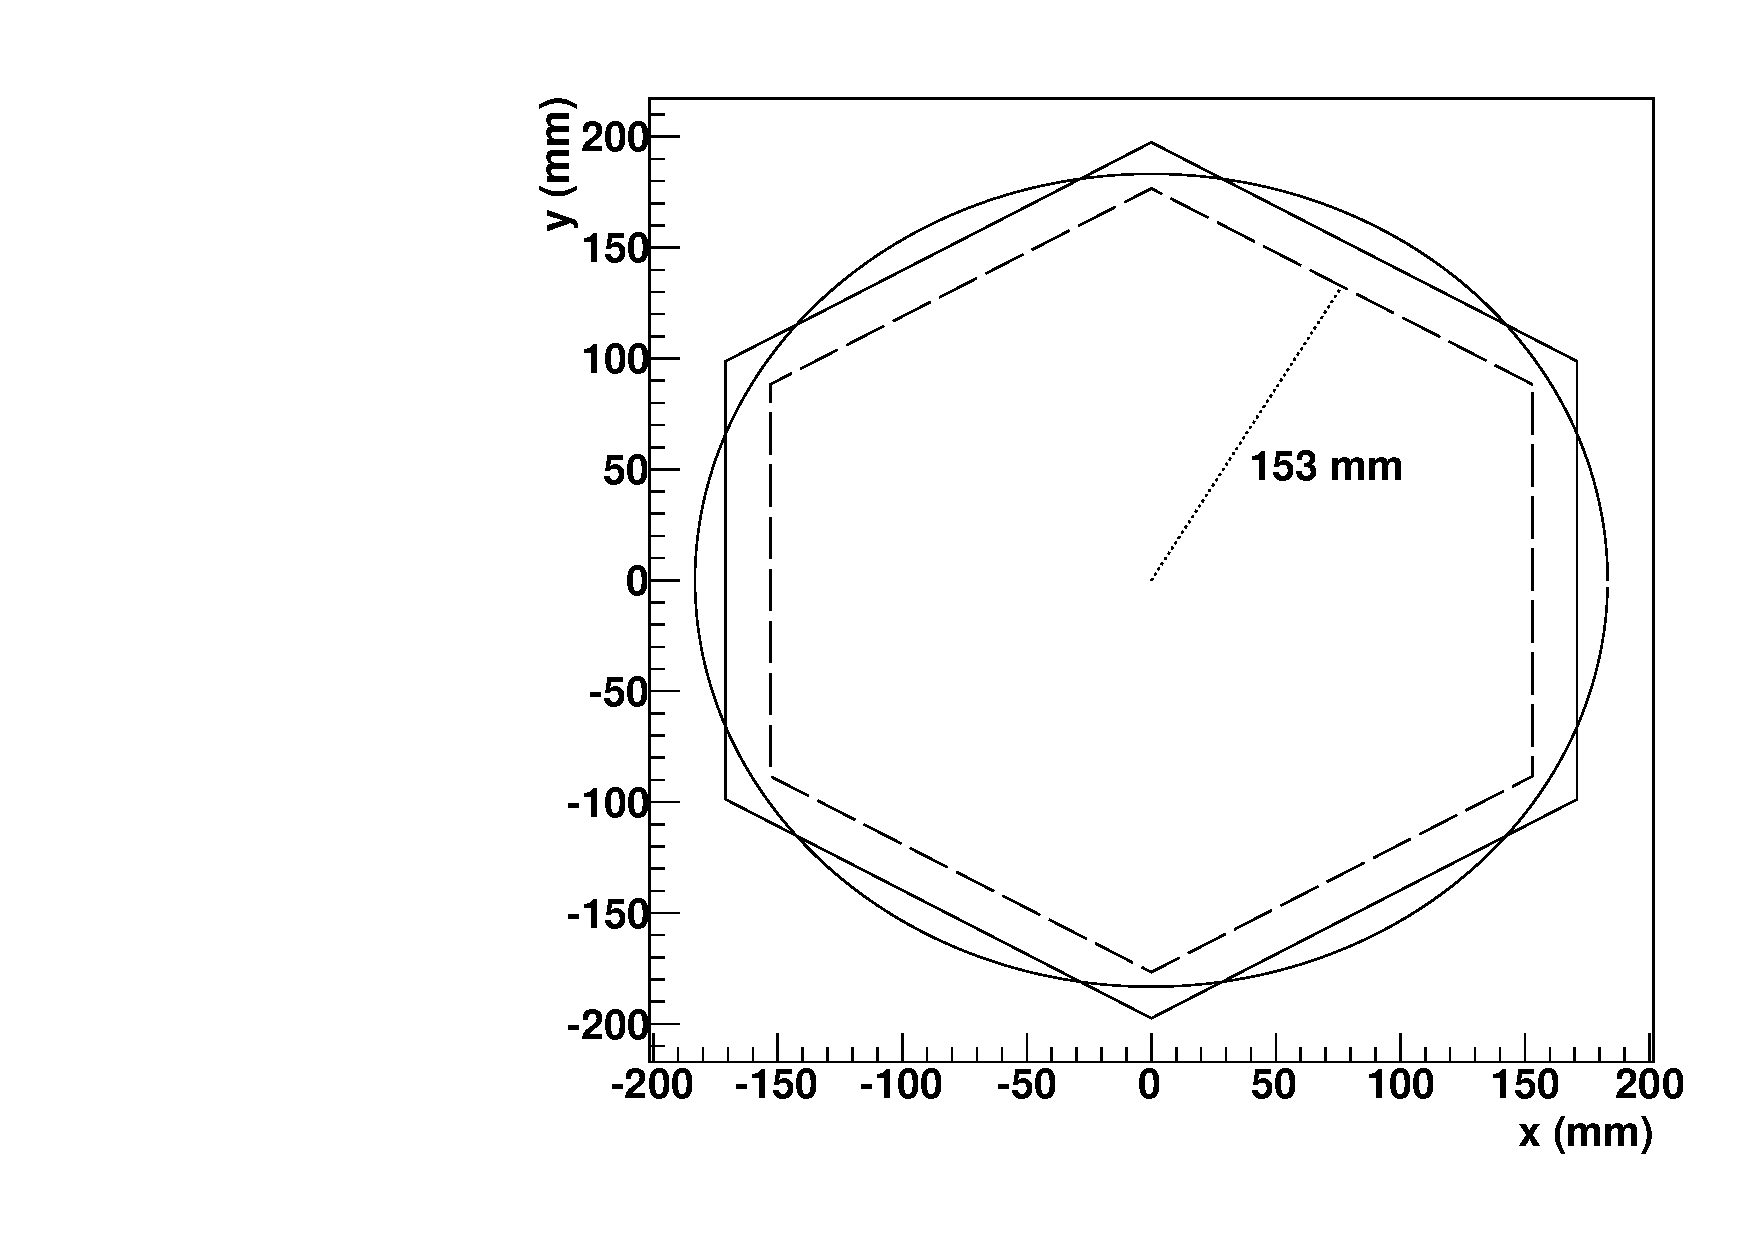
\includegraphics[width=\textwidth]{./plots/analysis_fiducial_vol_xy.pdf}
\end{subfigure}\hfill%
\begin{subfigure}[b]{0.48\textwidth}
	\centering
	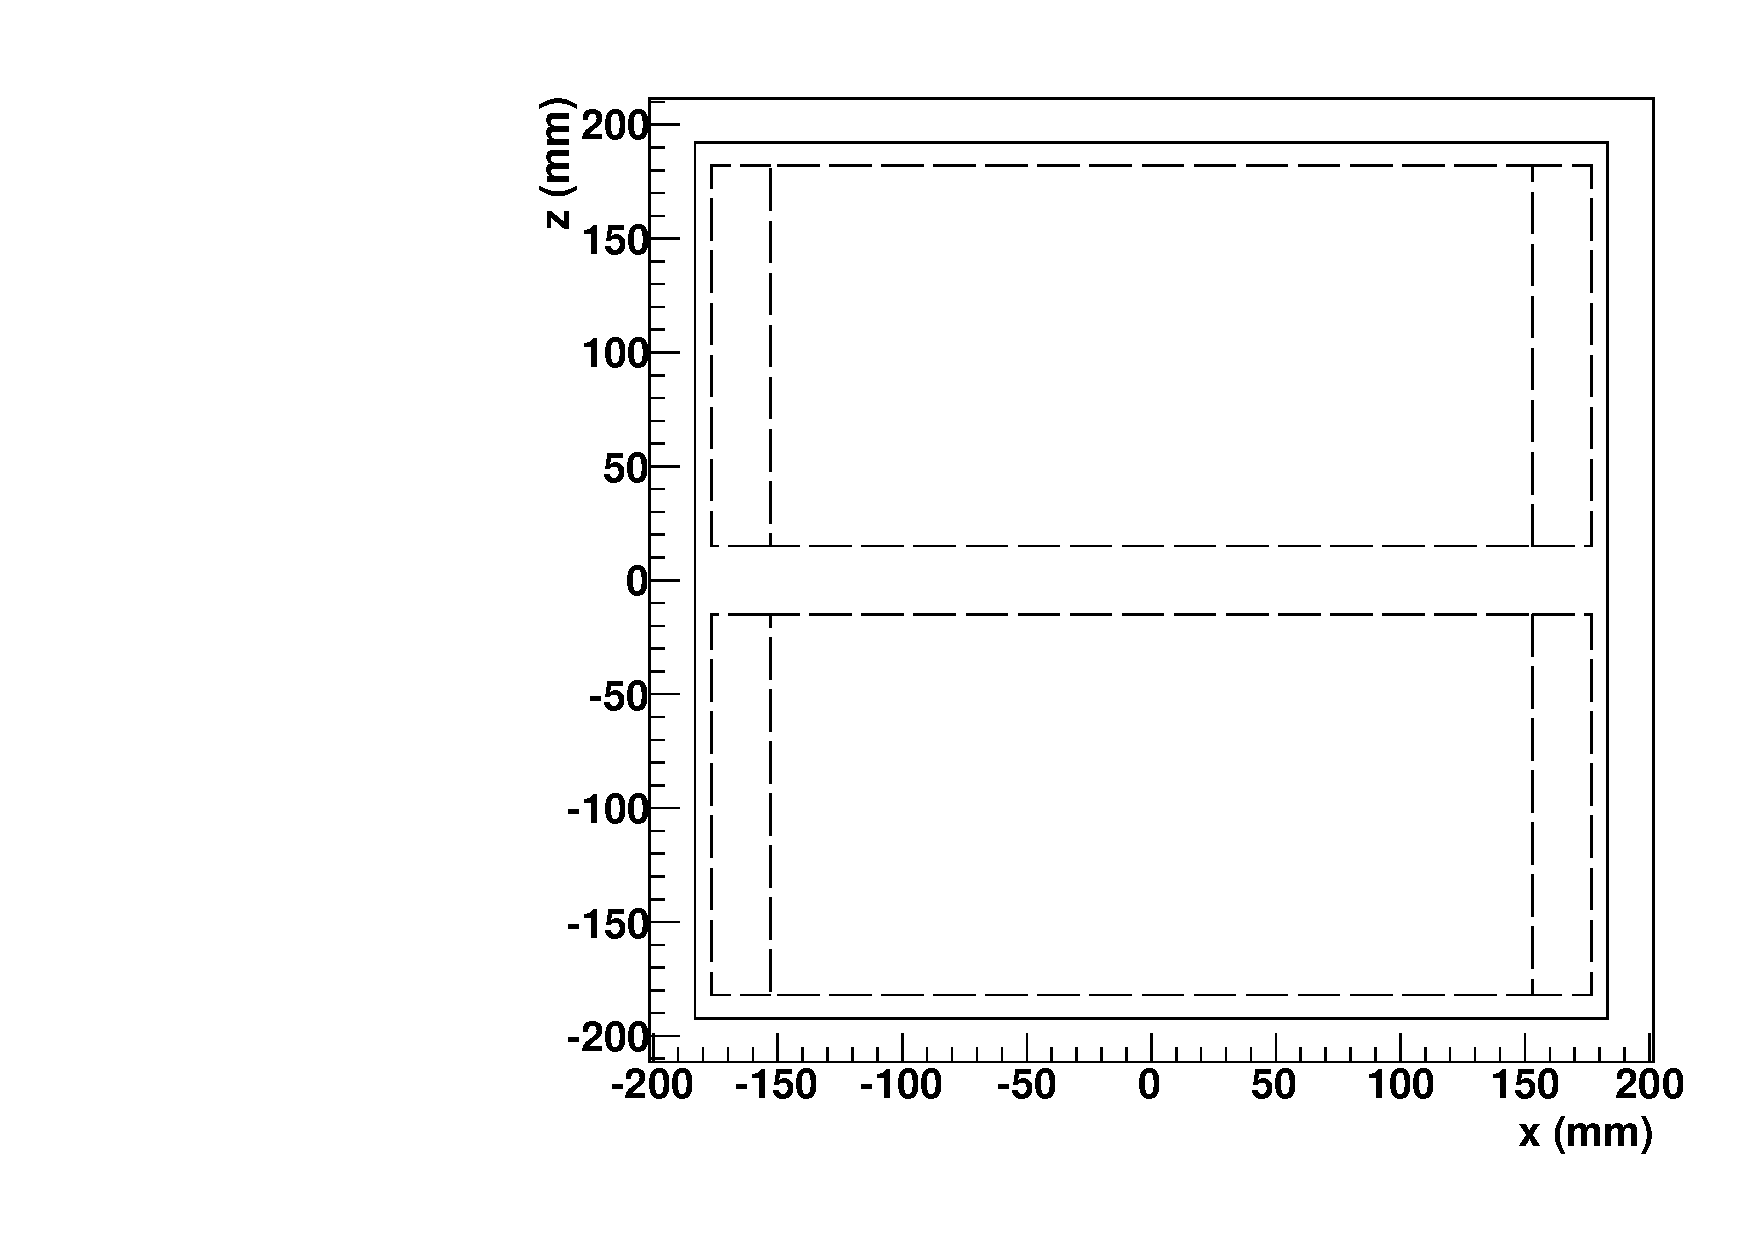
\includegraphics[width=1\textwidth]{./plots/analysis_fiducial_vol_xz.pdf}
	\end{subfigure}
\caption[Fiducial Volume]{Projections of the hexagonal fiducial volume. The dashed lines represent the fiducial volume. The solid lines are the anode wire plane and the teflon reflector. For the \(xz\) projection on the right, the two sets of vertical dashed lines are the maximum and minimum radial boundaries of the fiducial volume.}
\label{fig:analysis_fiducial_volume}
\end{figure}

All the liquid xenon within the teflon reflectors and between the anodes is ``active''. That is, ionization and scintillation in the active region are collected. However, only events within a fiducial volume are used in the analysis. This fiducial volume is a right hexagonal prism. The hexagon is coaxial with the detector and has apothem \SI{153}{\mm}. In each TPC, it begins \SI{5}{\mm} away from the cathode and extends to \SI{182}{\mm} (which is \SI{10.2}{\mm} from the \(v\) wire plane). \Cref{fig:analysis_fiducial_volume} provides an illustration. The total volume is \SI{27.1}{\litre}, which contains \SI{81.9}{\kg} of liquid xenon.

\begin{figure}[tbp]
\centering
	\begin{subfigure}[b]{0.48\textwidth}
	\centering
	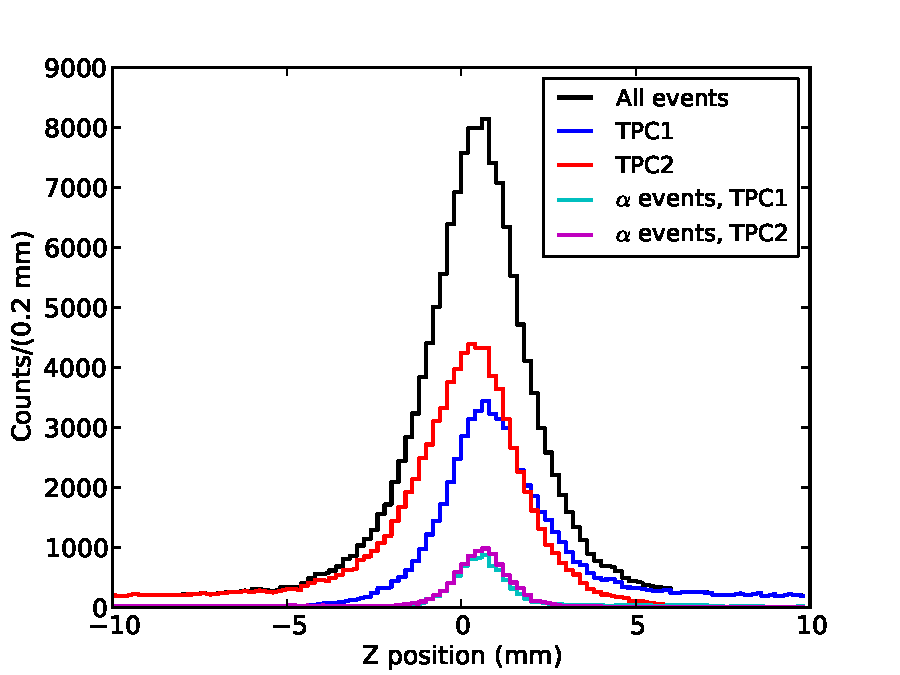
\includegraphics[width=\textwidth]{./plots/analysis_fiducial_vol_bg_cathode.pdf}
\end{subfigure}\hfill%
\begin{subfigure}[b]{0.48\textwidth}
	\centering
	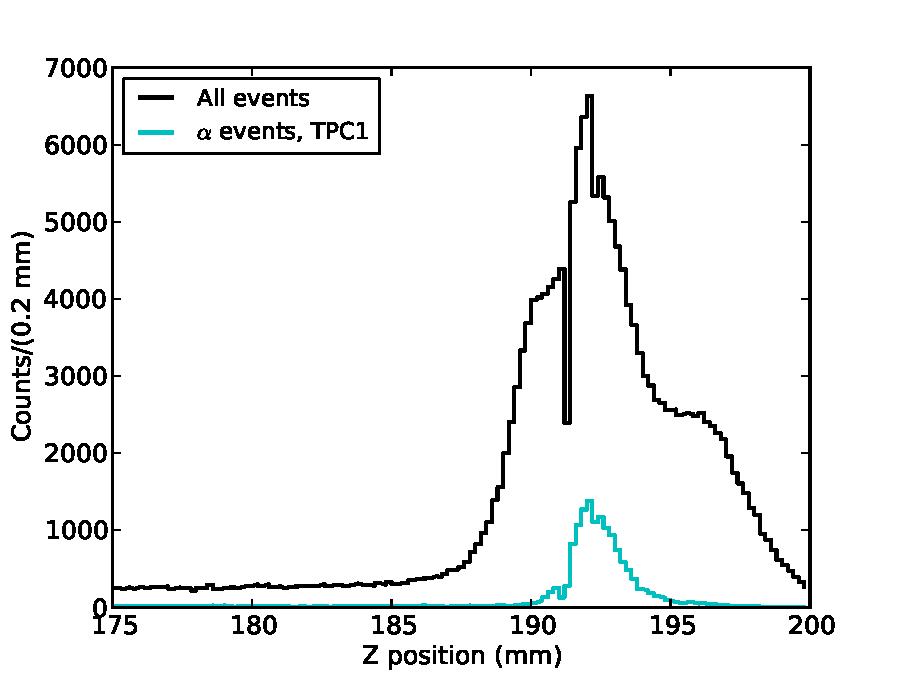
\includegraphics[width=1\textwidth]{./plots/analysis_fiducial_vol_bg_anode.pdf}
	\end{subfigure}
\caption[Increased event rates near cathode and anodes]{The choice of fiducial volume is partially motivated by the increased event rate seen near the cathode (at \(z = \SI{0}{\mm}\)) (shown left) and near the anodes (shown right; the \(v\) plane is at \(|z|=\SI{192}{\mm}\) and the \(u\) plane is at \(|z|=\SI{198}{\mm}\)). An increase is seen for both the total event rate, and for the rate of \(\alpha\) particle interactions, which suggests the increased rate is due to backgrounds. Requiring \(\SI{5}{\mm} < |z| < \SI{182}{\mm}\) puts the fiducial volume well away from the volumes that show an increased rate.}
\label{fig:analysis_fiducial_vol_bg_rates}
\end{figure}

This particular choice of fiducial volume has two chief motivations. The first is to reduce radioactive backgrounds from the detector materials. \Cref{fig:analysis_fiducial_vol_bg_rates} shows event rates near the cathode and anodes. There is nothing special about the xenon near these planes, and so the increased event rate must be due to backgrounds. The \(z\) cuts above eliminate the volumes that show higher-than-typical event rates.

\begin{figure}[tbp]
\centering
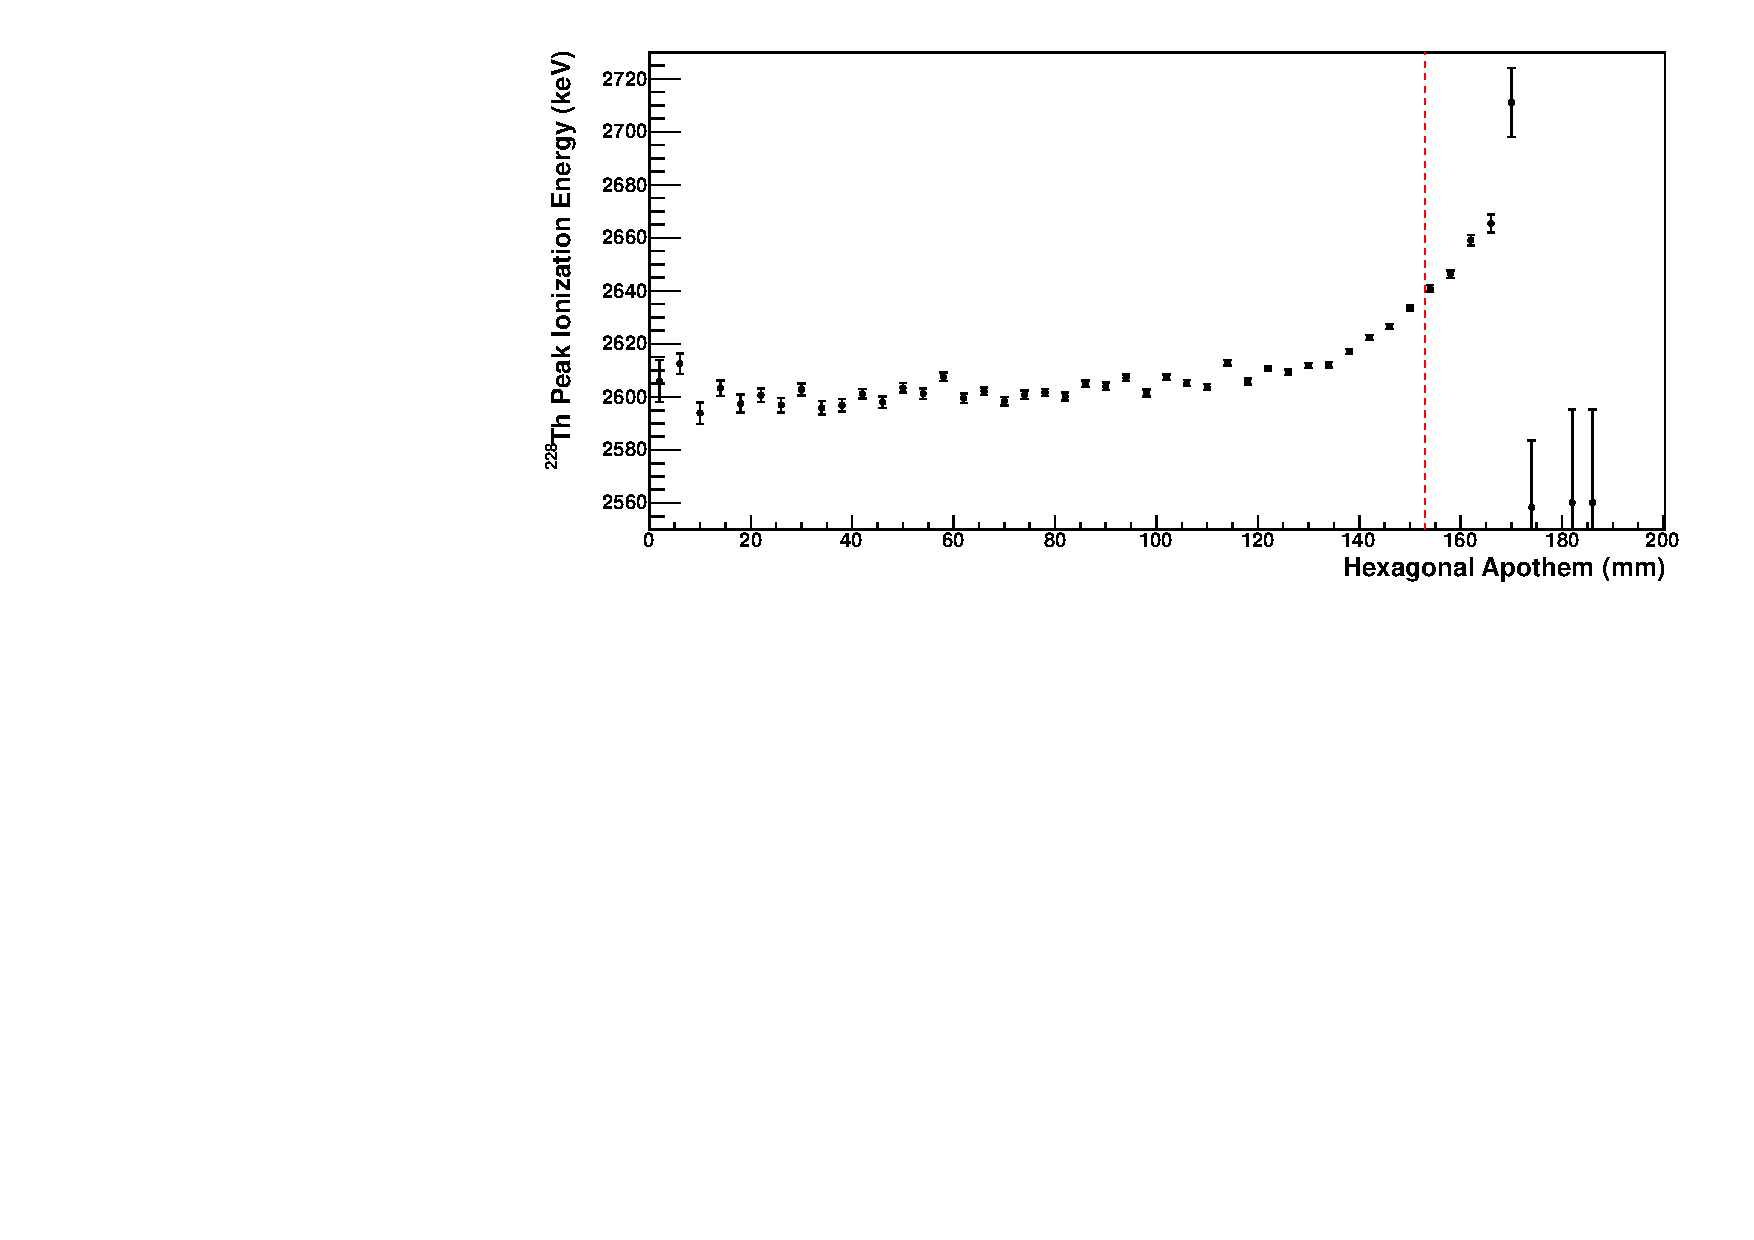
\includegraphics[width=0.9\textwidth]{./plots/analysis_fiducial_vol_transverse.pdf}
\caption[Energy response due to increasing fiducial volume apothem]{The reconstructed energy of the \SI{2615}{\keV} peak from a \isotope{228}{Th} source calibration. This is found by fitting a Gaussian + complimentary error function model to data with an increasingly large allowed fiducial volume. A larger allowed hexagonal apothem extends the fiducial volume closer and closer to the edges of the anode wire planes. The detector response begins to deviate significantly when the cut is extended above \SI{153}{\mm}, and so this is used to define the fiducial volume.}
\label{fig:analysis_fiducial_vol_transverse}
\end{figure}

The second motivation is to ensure a homogeneous detector response inside the fiducial volume. As shown in the previous discussion of the shielding grid correction in \cref{sec:data_grid_correction}, the correction becomes significant near \(|z|=\SI{182}{\mm}\) (see \cref{fig:data_grid_correction_fits}). Even with the correction applied, the detector response begins to diverge near that position (see \cref{fig:data_grid_correction_applied}), and so it is used as the boundary of the fiducial region. In the transverse dimension, a hexagonal cross-section is used. This matches the anode wire geometry, and so makes applying the fiducial volume cut straightforward. \Cref{fig:analysis_fiducial_vol_transverse} shows that requiring the apothem of this hexagon to be less than \SI{153}{\mm} ensures uniform energy response.

\subsection{Quantities of Interest}
\label{sec:analysis_quantities_of_interest}
Once an event passes the data quality cuts, the following quantities are calculated:
\begin{enumerate}
\item The multiplicity (single site or multiple site), using the criteria described in \cref{sec:data_topology}.
\item The event energy using the calibration obtained as described in \cref{sec:data_calibration}.
\item The ``standoff distance''. The radial distance of the cluster to the teflon reflector is calculated. So is the \(z\) distance to the \(v\) wire plane. The standoff distance is the minimum of these two distances. If multiple clusters are involved in the event, the minimum standoff distance of all clusters is used.
\end{enumerate}

The single site and multiple site information helps separate \(\gamma\) interactions from \(\beta\) interactions. The standoff distance describes the spatial distribution of events. For example, the distribution of \twonu{} events, since they are uniformly distributed in the detector, have a standoff distance distribution that extends to higher values. The distribution of background events from detector materials, on the other hand, peaks at small standoff distances. And, of course, the energy spectra of different types of decay are different.

\section{Monte Carlo Simulations of Signals and Backgrounds}
\label{sec:analysis_monte_carlo}

\subsection{Simulations}
\label{sec:analysis_simulations}
The GEANT4 simulation toolkit \cite{Agostinelli:2003fk} is used in order to determine both the energy spectra and spatial distributions of various double beta decay signals and radioactive backgrounds in EXO-200. The following are simulated using a detailed model of the detector and its surroundings (see \cref{fig:analysis_geant4_detector}):
\begin{itemize}
\item Double beta decay of \xenon{136}:
	\twonu{},
	\zeronu{},
	and \(0\nu\beta\beta\chi^{0}(\chi^{0})\) for spectral indices 1, 2, 3, and 7
\item Potential backgrounds in the liquid xenon:
	\xenon{135},
	%\item \xenon{137},
	and \isotope{222}{Rn}
\item Potential backgrounds in the detector copper:
	\isotope{40}{K}, 
	\isotope{54}{Mn},
	\isotope{60}{Co},
	\isotope{65}{Zn},
	\isotope{238}{U},
	and \isotope{232}{Th}
\item \isotope{222}{Rn} in the air gap between the cryostat and lead wall
\end{itemize}

For double beta decay and backgrounds in the liquid xenon, the events are simulated uniformly in the volume of active xenon. All double beta decay modes are simulated using the Fermi function by Schenter and Vogel \cite{Schenter:1983uq}. For \isotope{222}{Rn}, there are additional complications, however. Decays of radon and daughters in the inactive xenon can emit \(\gamma\) rays that also deposit energy in the active volume. Therefore, these are simulated as well. Additionally, charged radon daughters can drift to the cathode. \isotope{214}{Bi} emits \(\gamma\) rays when it decays. The daughter \isotope{214}{Po} has a \SI{164}{\micro\s} half-life, and so both are typically eliminated by the event-event coincidence and multiple scintillation cuts. However, on the cathode, the \(\alpha\) particle from the \isotope{214}{Po} decay may go into the cathode and not be seen. Therefore, \isotope{214}{Bi} on the cathode is simulated separately.

For backgrounds in the detector copper, the TPC vessel, all internal components, the legs, and the high-voltage feedthrough are simulated as a whole. These are all modeled in the simulation, as shown in \cref{fig:analysis_geant4_detector}. It is assumed that the impurities are uniformly distributed according to copper mass. Even if some of the contamination is distributed according to surface area, the thin-walled construction of EXO-200 makes this a close approximation.

\begin{figure}[htbp]
\centering
	\begin{subfigure}[c]{0.58\textwidth}
	\centering
	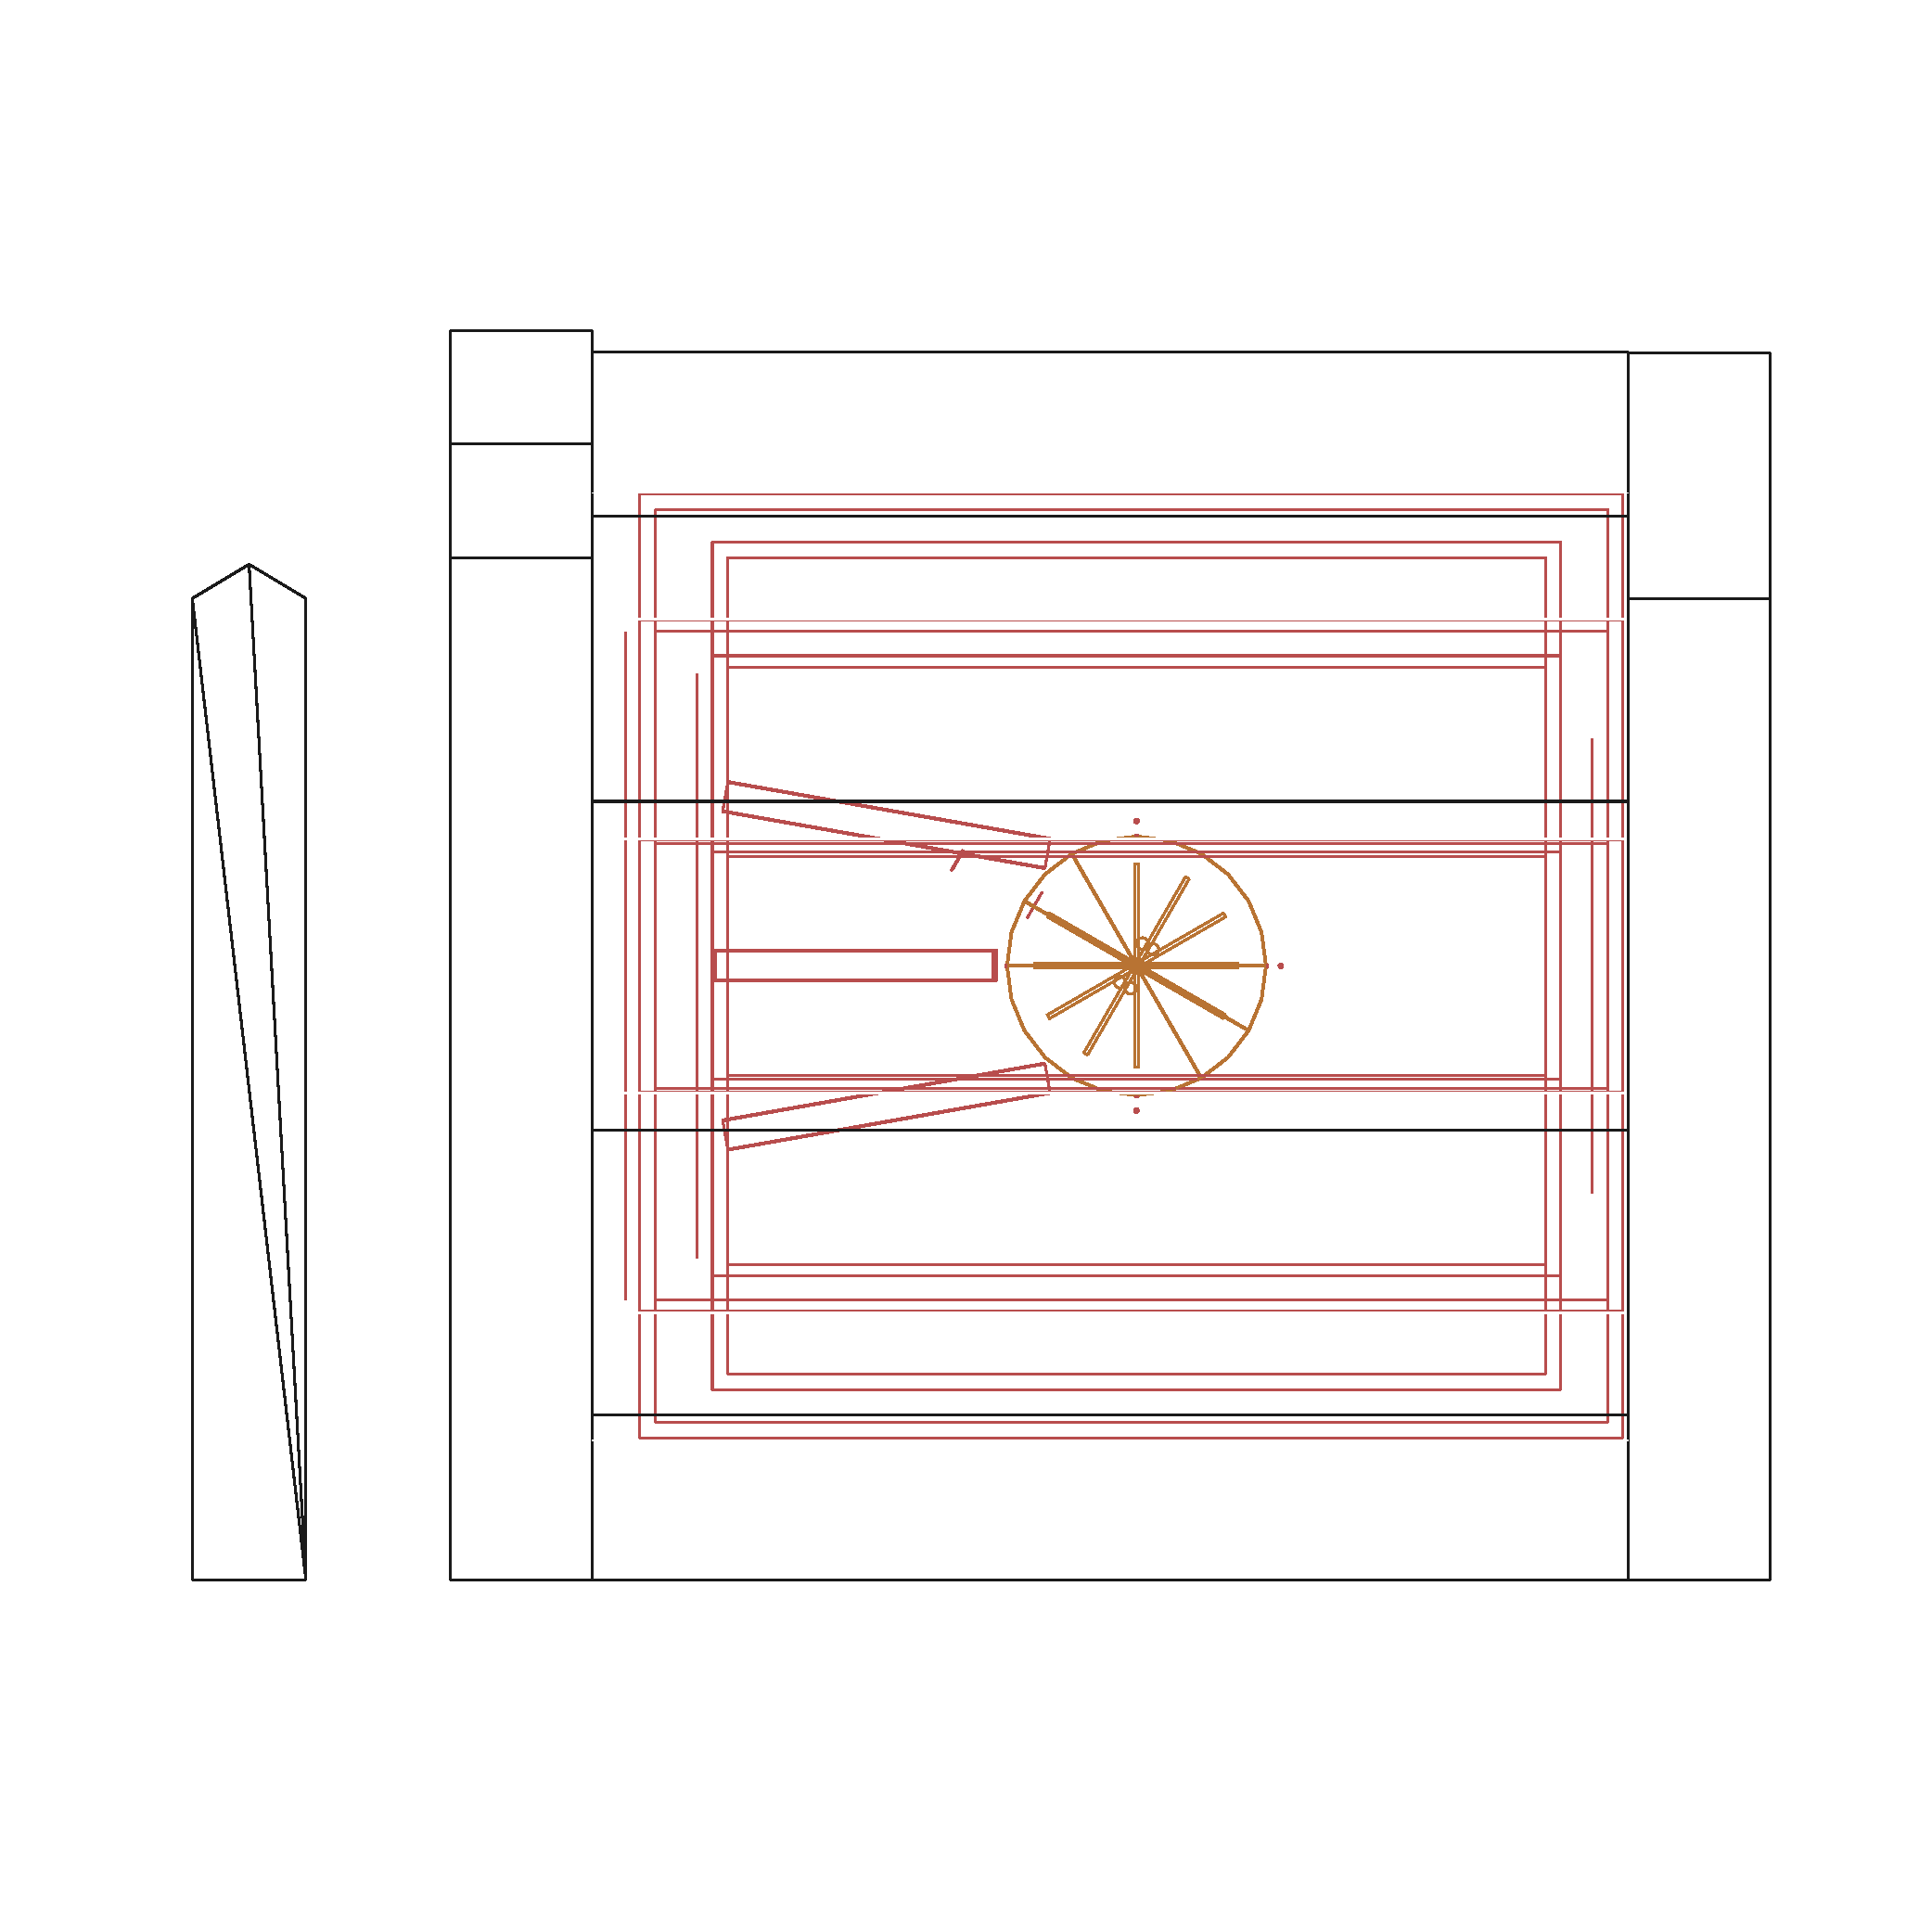
\includegraphics[width=\textwidth]{./plots/analysis_geant4_geometry_cropped.pdf}
	\end{subfigure}\hfill%
	\begin{subfigure}[c]{0.38\textwidth}
	\centering
	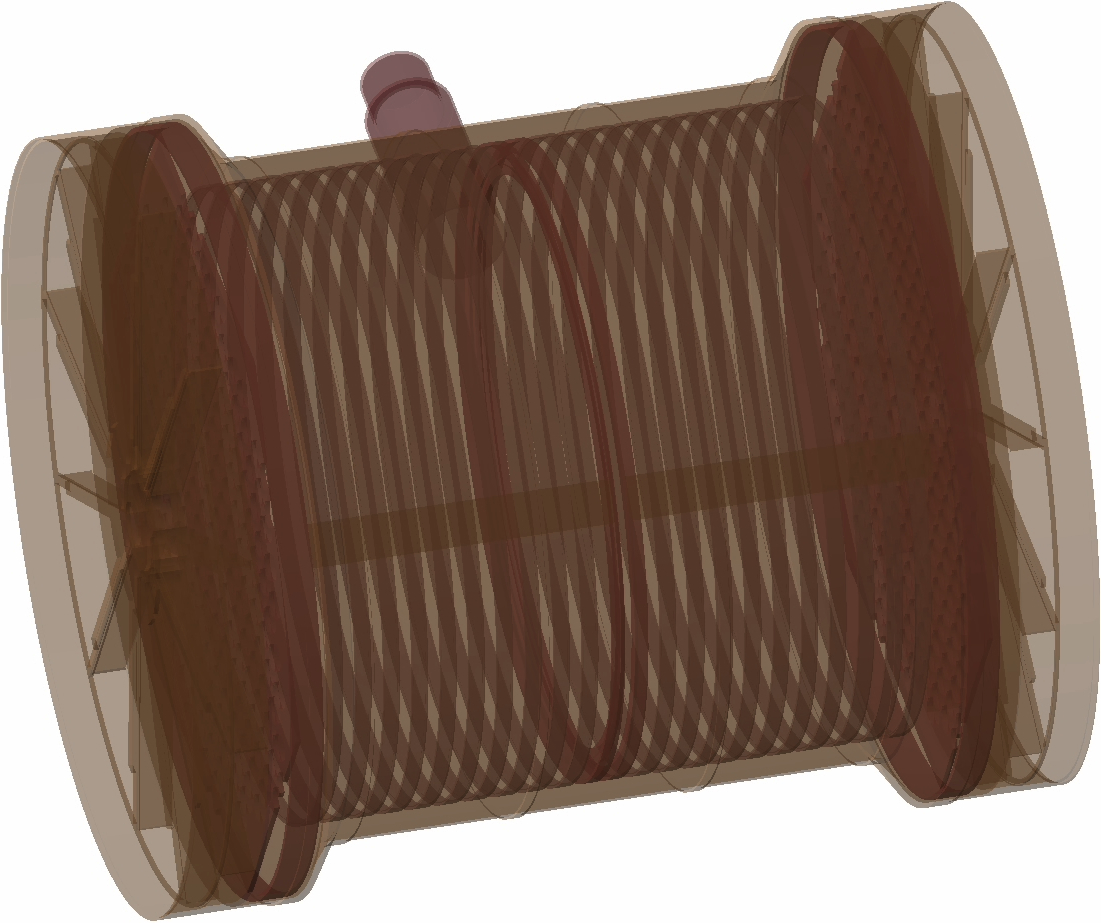
\includegraphics[width=\textwidth]{./photos/analysis_geant4_TPC_cropped.png}
	\end{subfigure}
\caption[EXO-200 geometry simulated in GEANT4]{EXO-200 as implemented in GEANT4 for simulations. The geometry incorporates the lead shielding, cryostat, HFE, and detector (shown left). The detector itself (shown right) is quite detailed in order to accurately simulate backgrounds from the detector materials.}
\label{fig:analysis_geant4_detector}
\end{figure}

%In principle, backgrounds in the HFE and cryostat walls should also be simulated. However, these spectra are similar to those resulting from simulations in the detector copper. With the number of events observed by EXO-200 in the Run2a data, there is not enough statistical power to distinguish backgrounds in the detector copper from backgrounds in other, nearby materials.

%Few external backgrounds (chiefly due to \isotope{40}{K}, \isotope{232}{Th}, and \isotope{238}{U} in the mine's salt walls) can penetrate the lead shielding and HFE. One notable exception is \isotope{222}{Rn}, which can exist in the air between the cryostat and lead walls. Some \(\gamma\) rays from the \isotope{214}{Bi} daughter can penetrate into the detector volume, and so this background is simulated.

\subsection{PDF Generation}
For a single event, the GEANT4 simulation provides a list of energy deposits in the liquid xenon, their positions, and their times. These must then be converted into simulations of the signals actually seen by the detector. This begins by estimating the amount of drifting ionization by using the \SI{15.6}{\eV} \(W\)-value (see \cref{sec:xe_ionization}) and the observation that \about{}\SI{80}{\percent} of ionization drifts instead of recombining in strong electric fields \cite{Aprile:1991fk}. \(\alpha\) particles have their ionization yield quenched by a factor of 0.055 \cite{Aprile:1991uq}. This ionization is drifted to the anodes in small time steps, and the signals on the wires are determined using the Shockley-Ramo theorem using a 2D MAXWELL simulation of the electric fields in the detector.

The energy that doesn't go into drifting ionization goes into scintillation. The anticorrelation between ionization and scintillation is not modeled, and so the fraction of energy in scintillation is constant. The scintillation photons are distributed across the two planes in a parameterized way. All photoelectrons from the APDs are assumed to arrive instantaneously, since the scintillation signal arrives in \si{\ns}, compared to the \si{\micro\s} digitization time.

White noise is added to the ionization and scintillation signals to yield a similar signal-to-noise ratio as in the detector. They are then run through simulations of the shapers found in the detector electronics, and are digitized at \SI{1}{\MHz}, just as the real signals. The matched filter and multiple signal finder are applied to identify signals, and the signals are bundled and clustered. The process is identical to the one described in \cref{sec:data_reconstruction}. This simulates the efficiency and energy threshold effects that come from signal-finding and reconstruction, as well as the position resolution.

The final step is to form distributions in multiplicity, energy, and standoff distance that can be fit to the data collected by the detector. The multiplicity and standoff distance can be calculated directly from the reconstruction described above. For the energy, however, the true energy from Monte Carlo simulation is used. For each cluster found by the reconstruction process, the energy deposits that arrived on the wires associated with the cluster at the appropriate time are summed to get the cluster's true energy.

In order to simulate the detector energy resolution, the true energies are smeared by a parameterized resolution function given by
\begin{equation}
\frac{\sigma(E)}{E} = \sqrt{\frac{p_0^2}{E^2} + \frac{p_1^2}{E} + p_2^2}
\label{eq:analysis_energy_resolution}
\end{equation}
where \(p_0\) is a constant, noise-like smearing, \(p_1\) is a smearing due to counting statistics, and \(p_2\) is an energy-dependent smearing that can be due to drifting gains or other inhomogeneities. These parameters are determined for the entire data set by fitting a simulated calibration source spectrum to the calibration data collected by the detector during the entire time period. The values of the parameters are shown in \cref{tab:analysis_resolution_parameters}, and the resolution as a function of energy is shown in \cref{fig:analysis_resolution}.

\begin{table}[htbp]
\centering
\caption[Energy resolution parameters]{The values for the energy resolution parameters used in this analysis for both single site (SS) and multiple site (MS) events. The parameters are defined in \cref{eq:analysis_energy_resolution}.}
\label{tab:analysis_resolution_parameters}
\begin{tabular}{c c c c}\toprule
Multiplicity	&	\(p_0\) (\si{\keV})	&	\(p_1\) (\(\sqrt{\si{\keV}}\))		&	\(p_2	\)		\\\midrule
SS			&	39.2				&	\num{7.0e-4}				&	0.01			\\
MS			&	40.9				&	\num{2.8e-4}				&	0.01			\\\bottomrule
\end{tabular}
\end{table}

\begin{figure}[tbp]
\centering
	\begin{subfigure}[b]{0.48\textwidth}
	\centering
	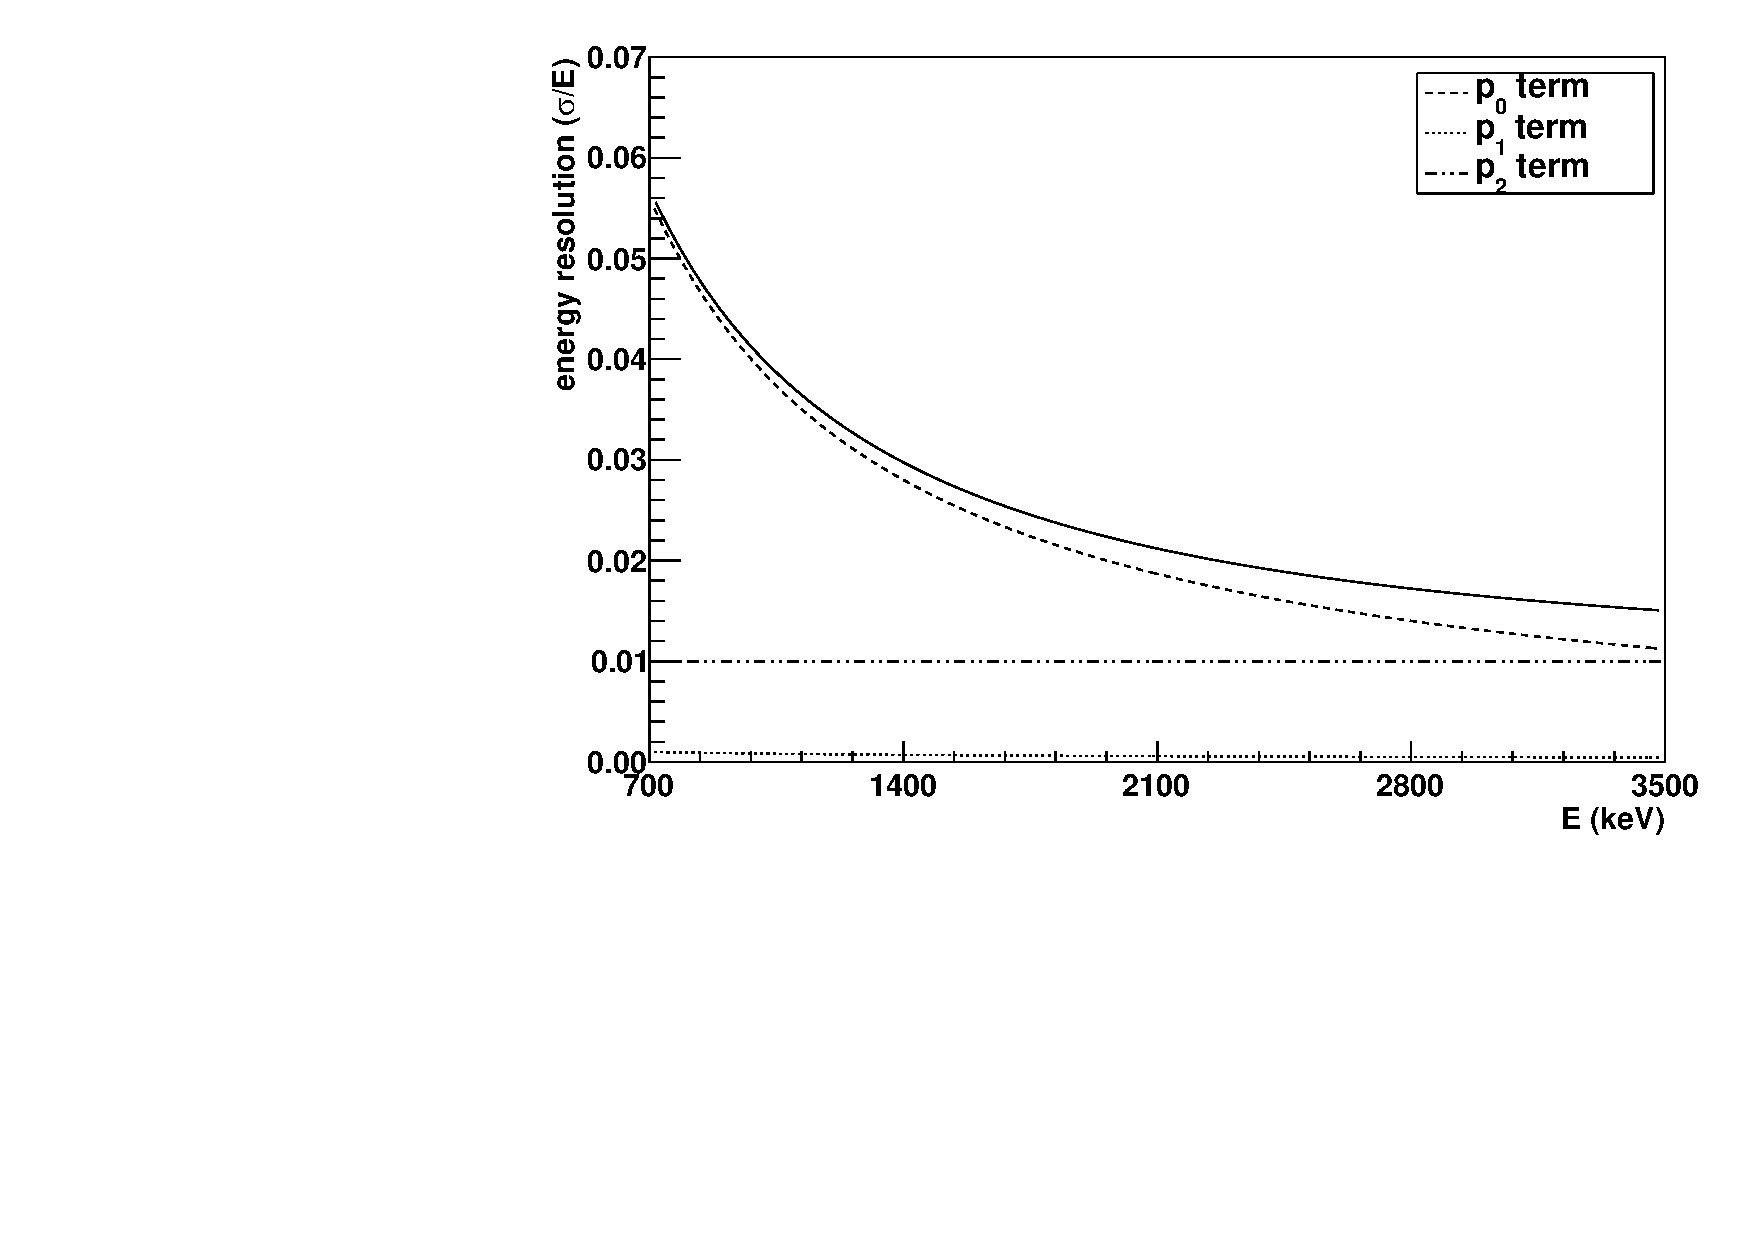
\includegraphics[width=\textwidth]{./plots/analysis_resolution_ss.pdf}
	\end{subfigure}\hfill%
	\begin{subfigure}[b]{0.48\textwidth}
	\centering
	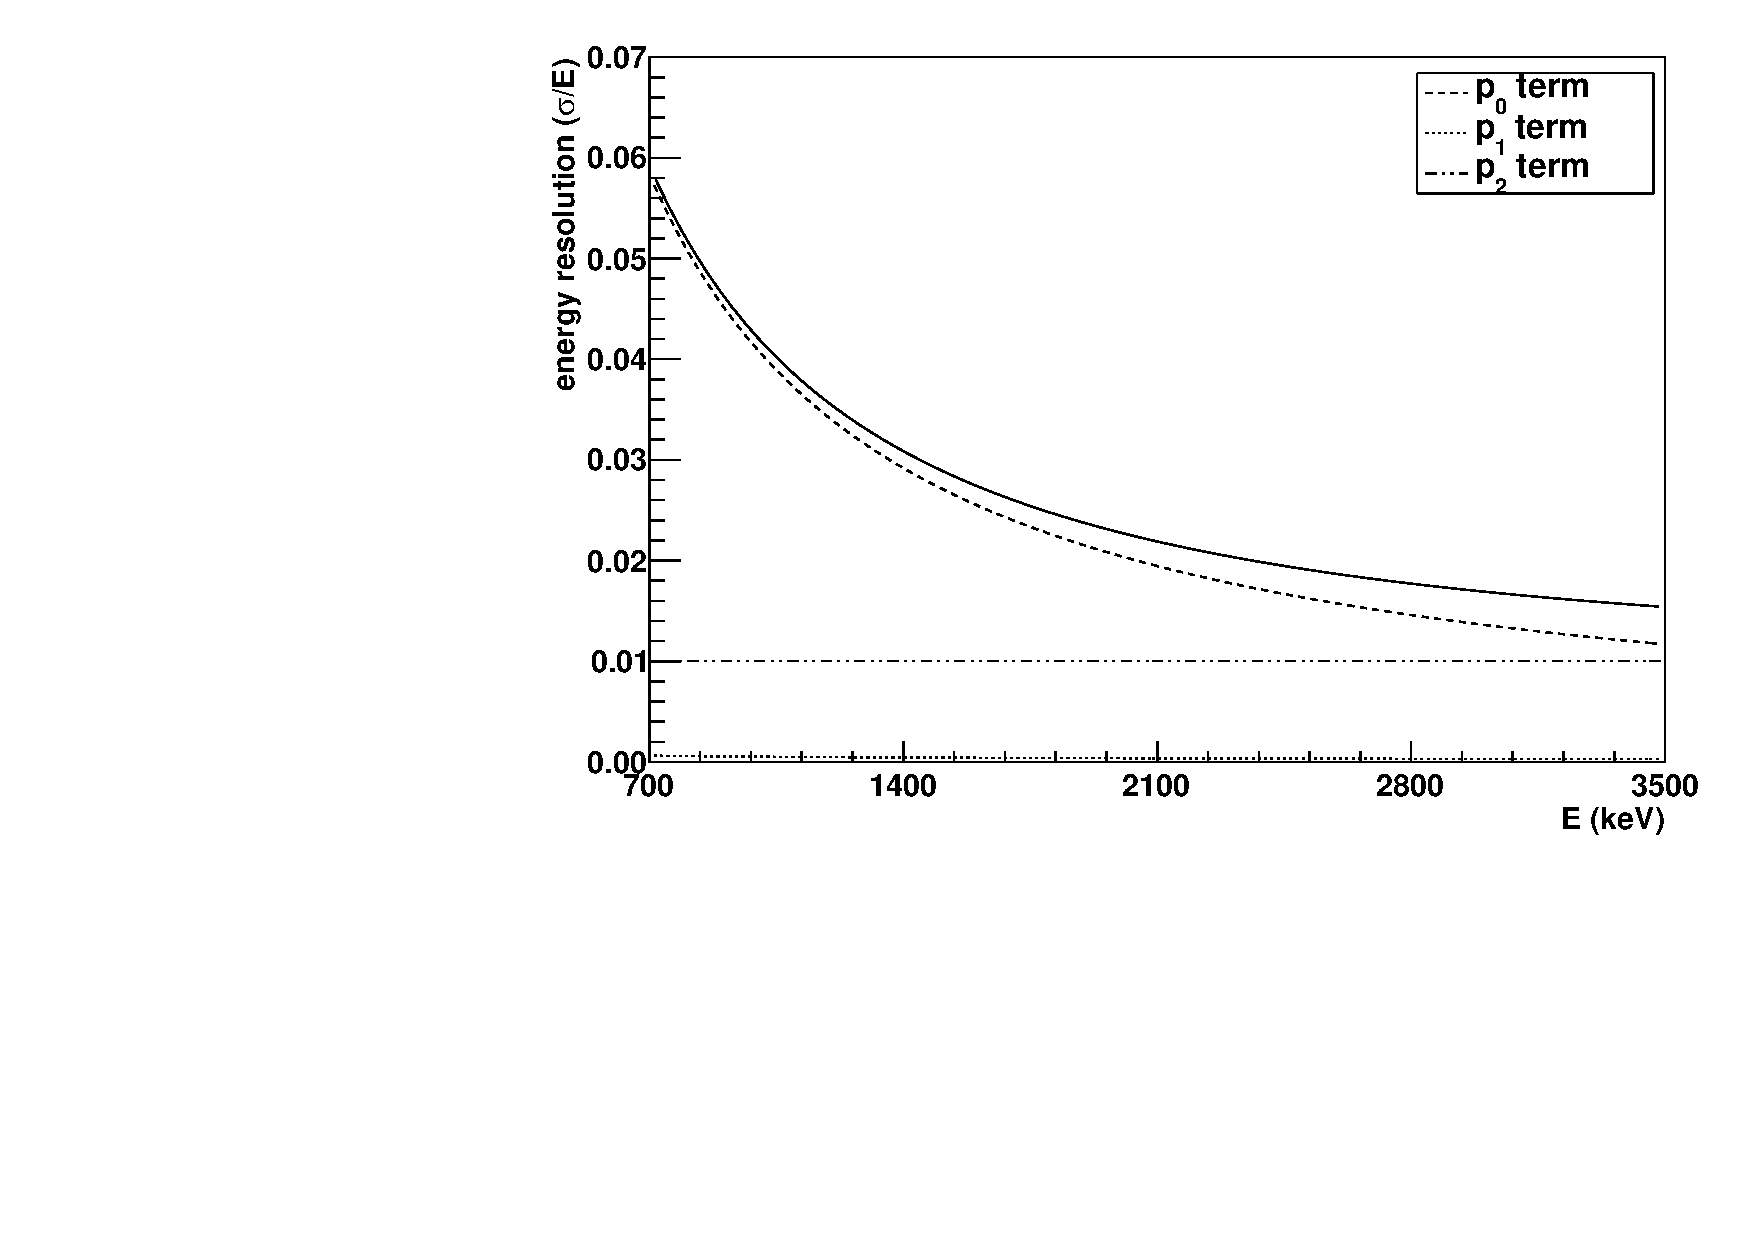
\includegraphics[width=\textwidth]{./plots/analysis_resolution_ms.pdf}
	\end{subfigure}
\caption[Parameterized energy resolution functions]{The parameterized energy resolution as a function of energy for single site (left) and multiple site (right) events. The dark curve is the resolution, while the various dashed lines show the contributions of the individual terms. This is determined by finding the set of parameters that best match a simulated spectrum to the spectrum obtained in calibration runs.}
\label{fig:analysis_resolution}
\end{figure}

The true energies from the signal and background Monte Carlo simulations are smeared according to the parameterization in \cref{eq:analysis_energy_resolution}. For each simulation, two probability density functions (PDFs) are formed in energy and standoff distance: one for single site events, and one for multiple site events. \Cref{fig:analysis_example_PDFs} shows an example of two smeared PDFs. For each simulation, the efficiency for a simulated event to make it into the final PDFs is recorded, as well as the fractional split between single site and multiple site events.

\begin{figure}[htbp]
\centering
	\begin{subfigure}[b]{0.48\textwidth}
	\centering
	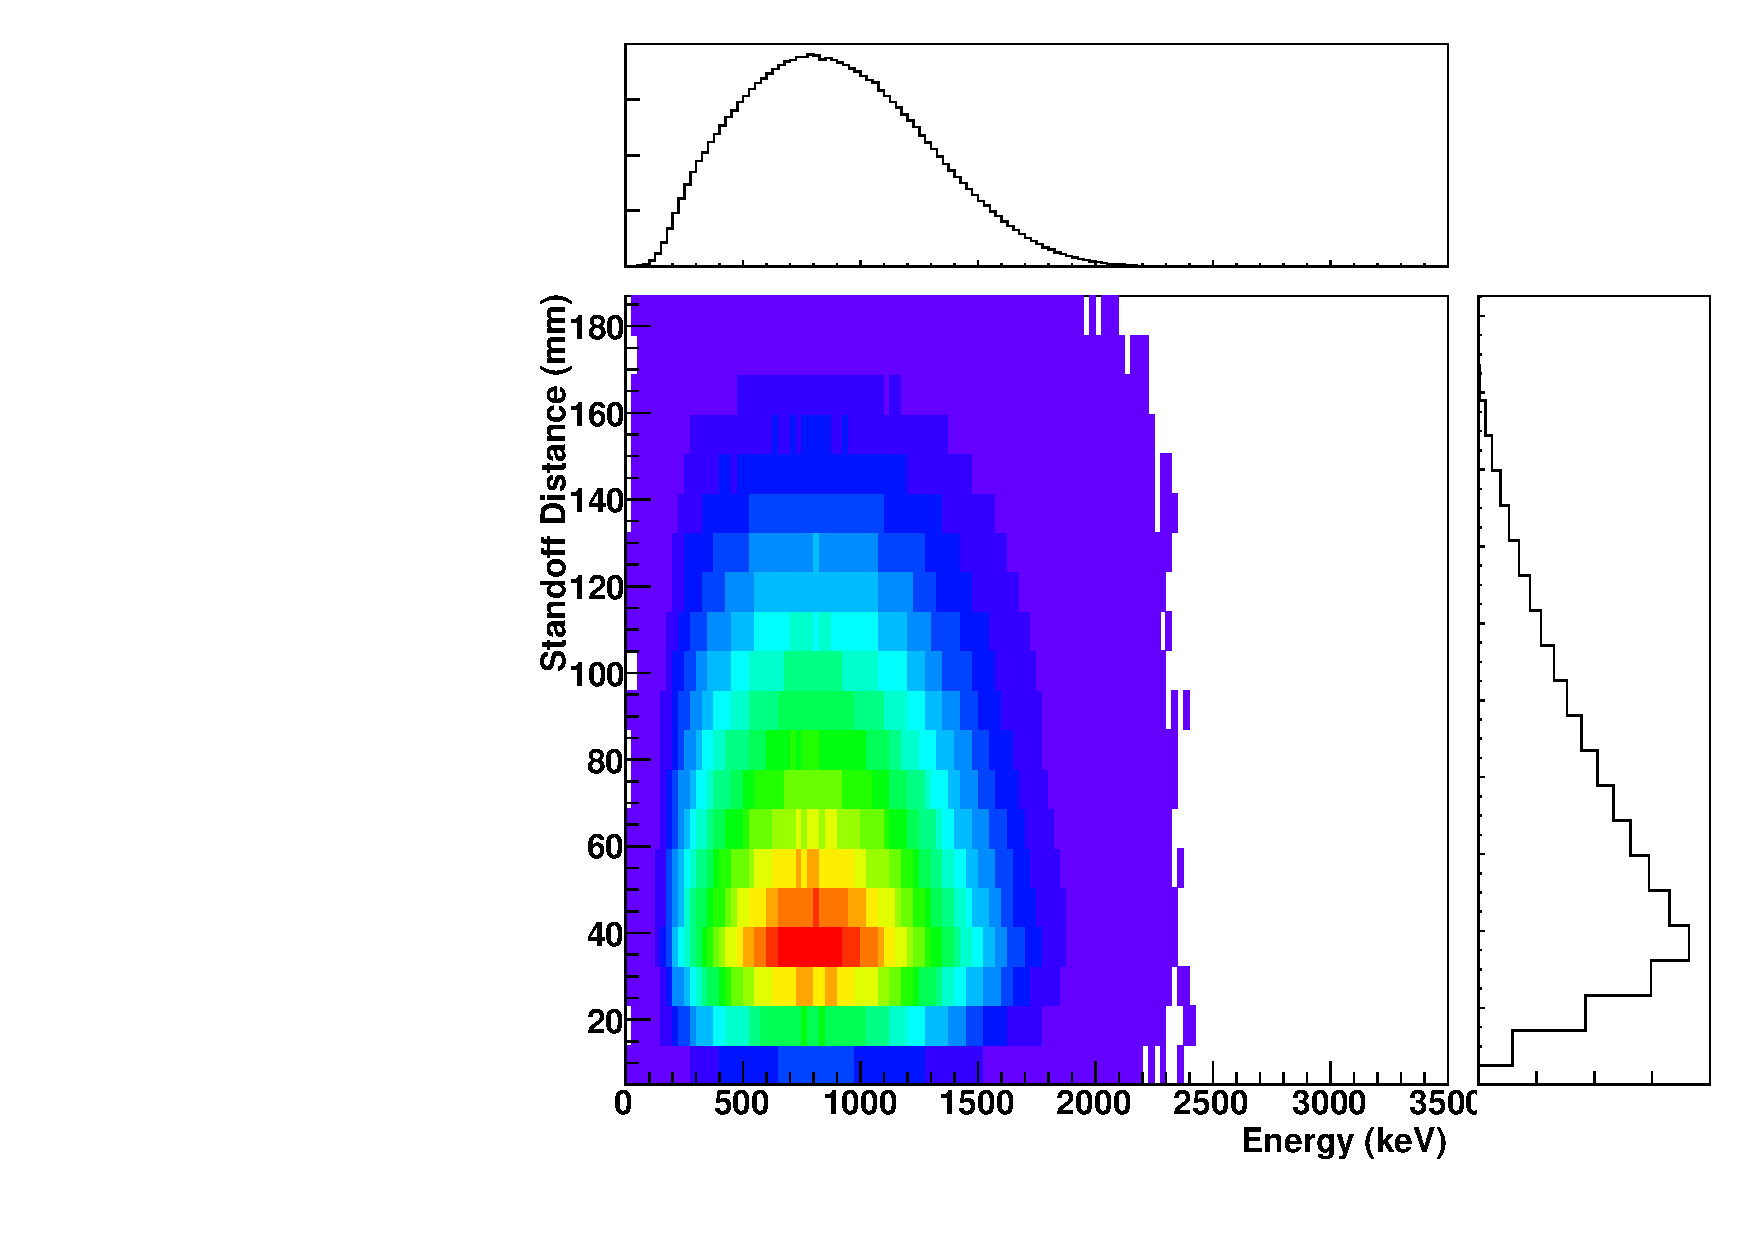
\includegraphics[width=\textwidth]{./plots/PDFs/analysis_pdf_bb2n_ss.pdf}
	\end{subfigure}\hfill%
	\begin{subfigure}[b]{0.48\textwidth}
	\centering
	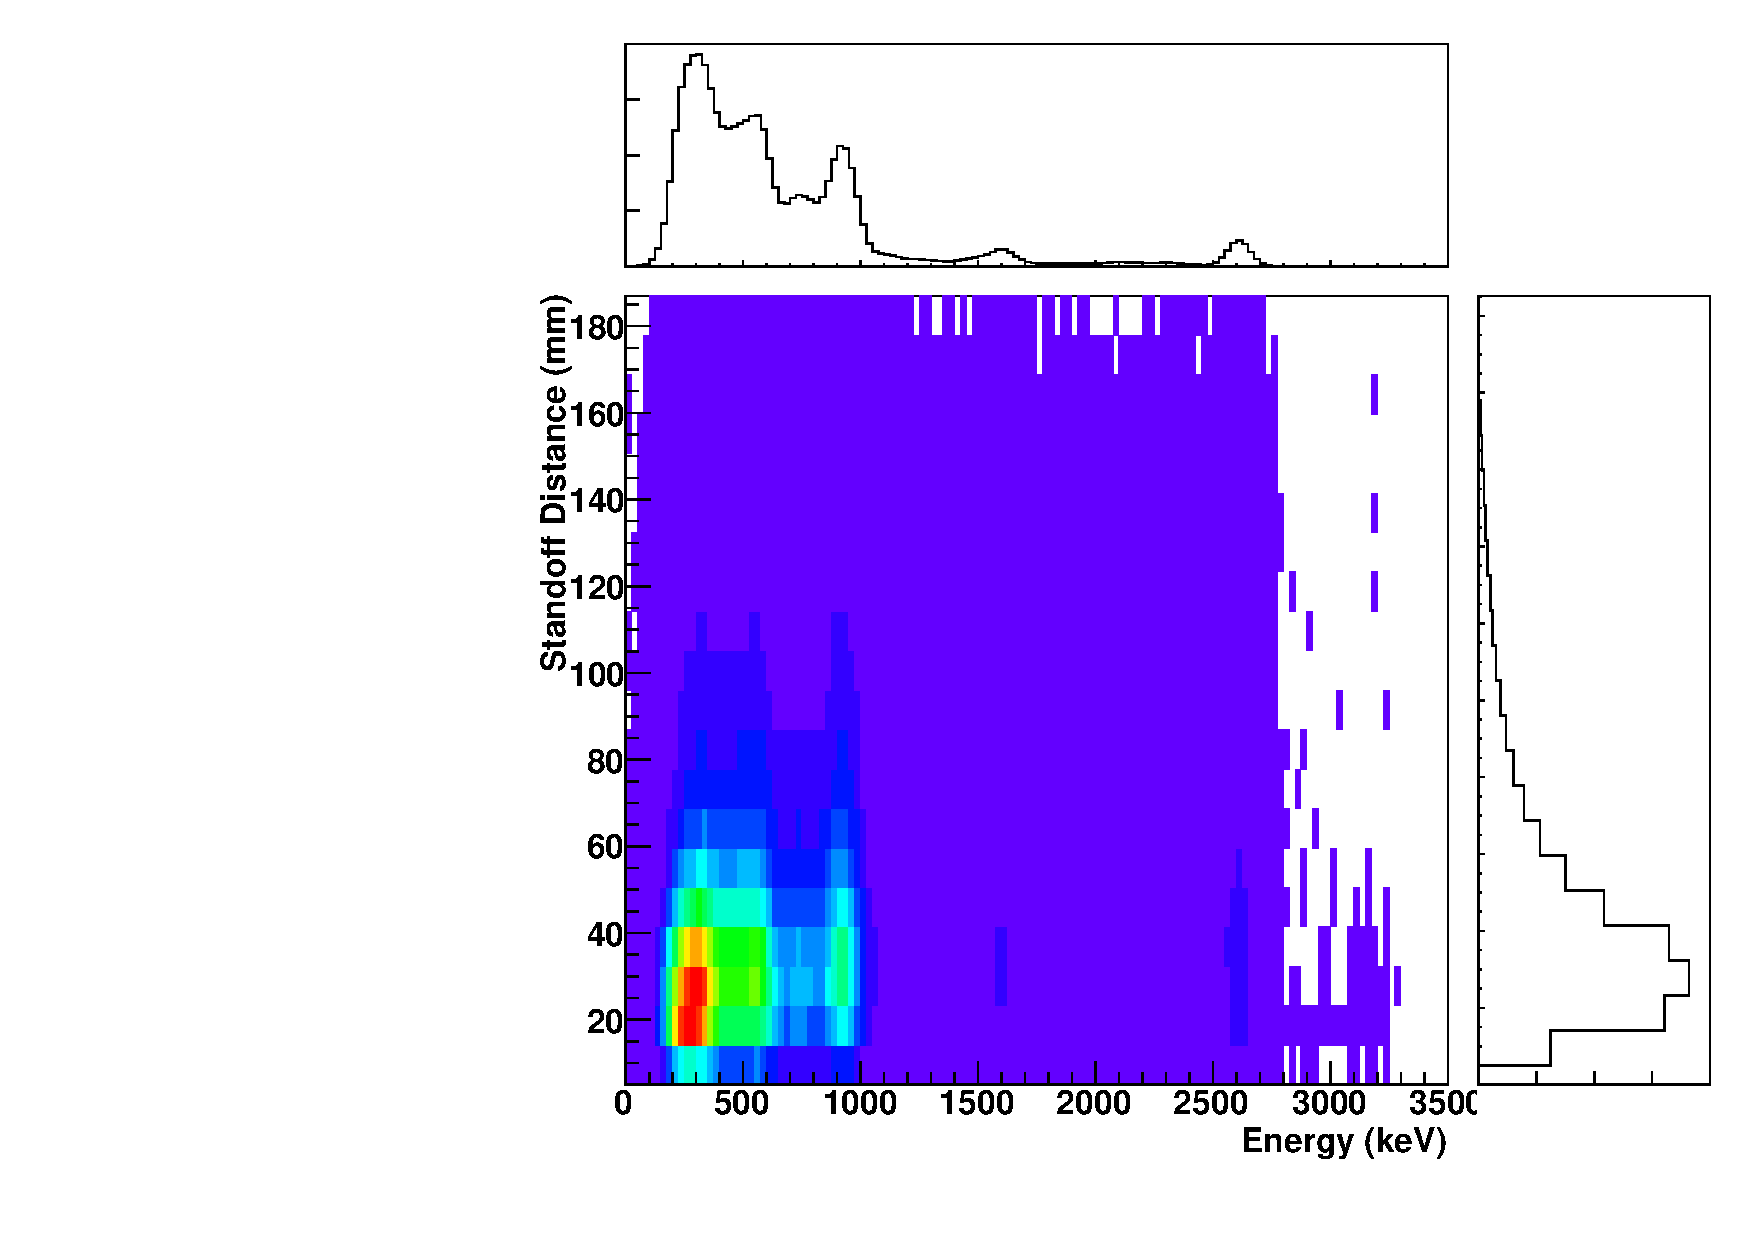
\includegraphics[width=\textwidth]{./plots/PDFs/analysis_pdf_AllVessel_Th232_ss.pdf}
	\end{subfigure}
	\begin{subfigure}[b]{0.48\textwidth}
	\centering
	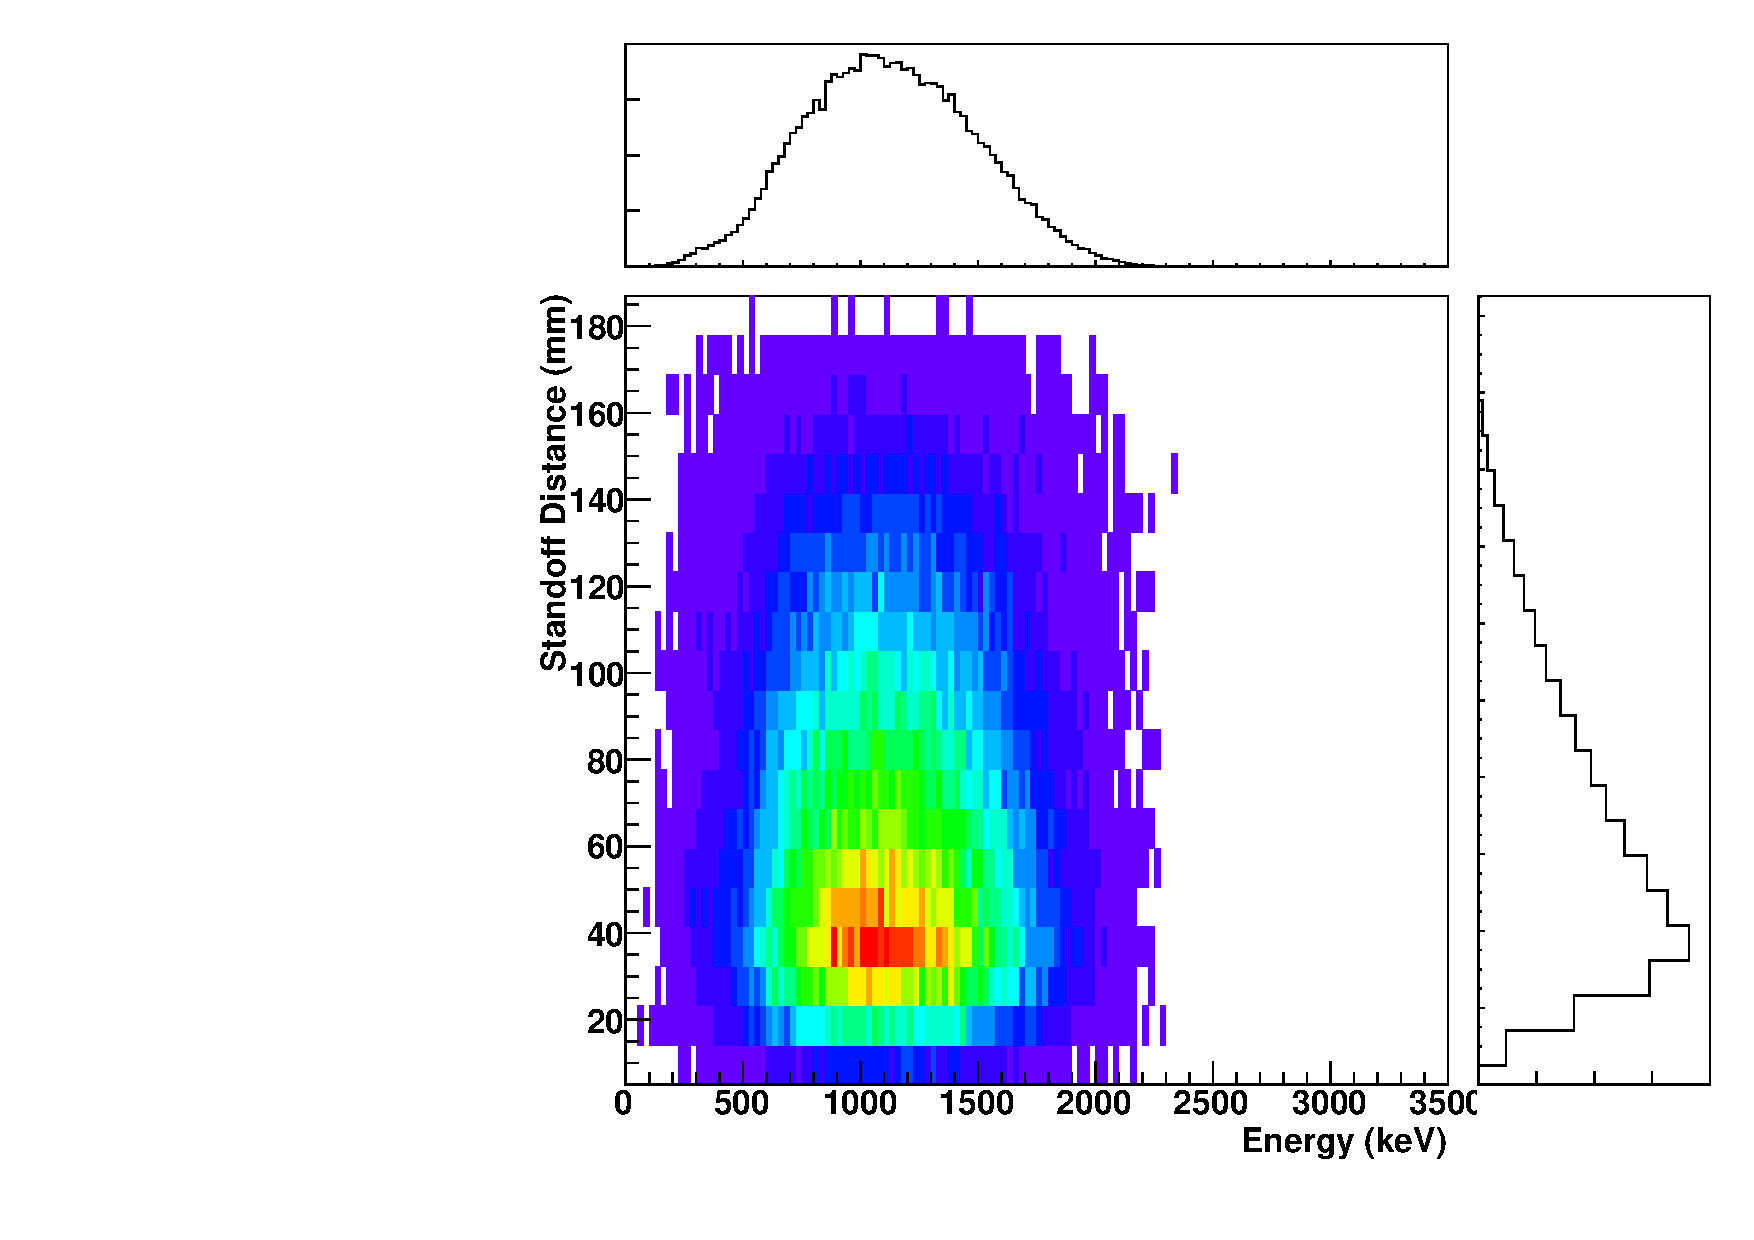
\includegraphics[width=\textwidth]{./plots/PDFs/analysis_pdf_bb2n_ms.pdf}
	\end{subfigure}\hfill%
	\begin{subfigure}[b]{0.48\textwidth}
	\centering
	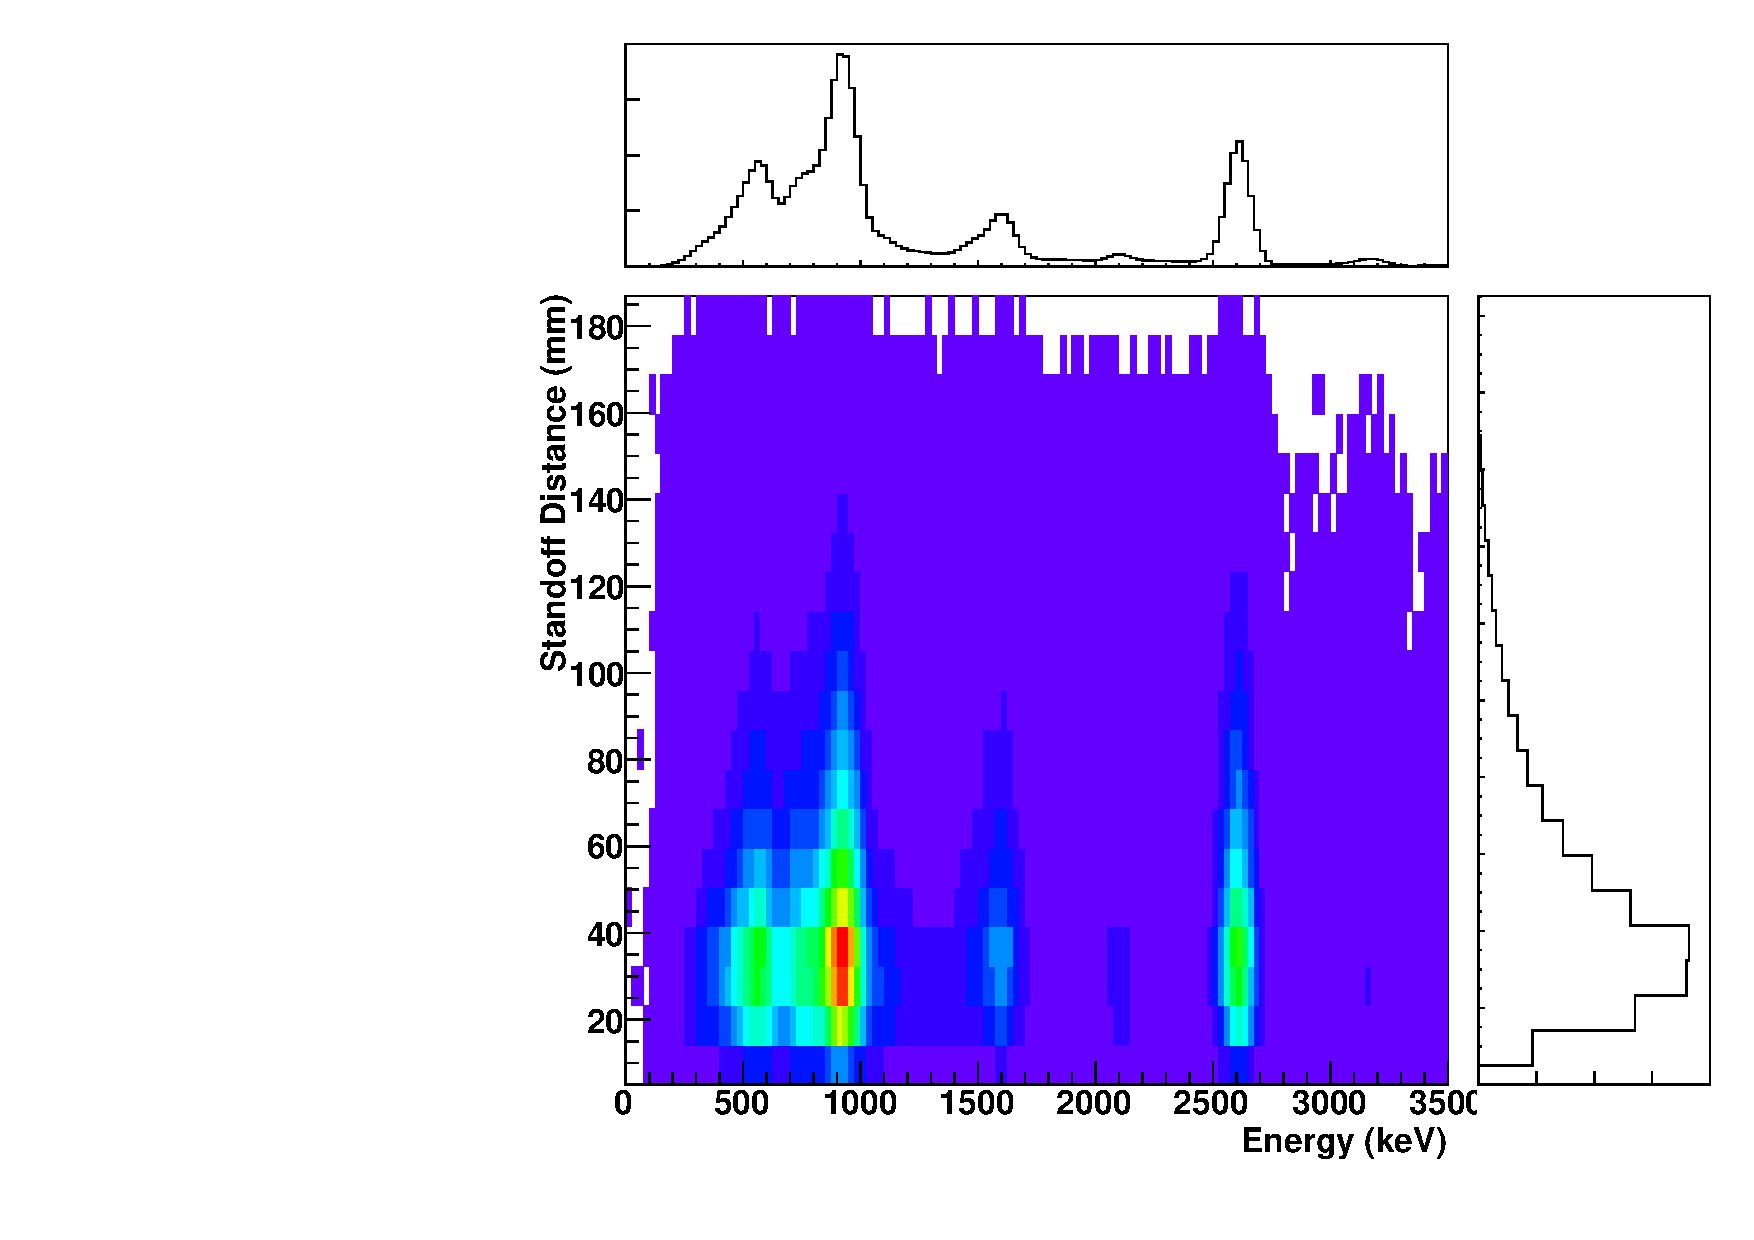
\includegraphics[width=\textwidth]{./plots/PDFs/analysis_pdf_AllVessel_Th232_ms.pdf}
	\end{subfigure}
\caption[Examples of 2D PDFs]{Two-dimensional PDFs generated by the Monte Carlo simulations described in the text. On the left is the spectrum for \twonu{}, and on the right is the spectrum for \thorium{232} in copper of the TPC vessel. On top are the single site spectra, while multiple site spectra are on the bottom. The vertical axis in all plots is the standoff distance, while the horizontal axis is energy. 1D projections in energy and standoff distance are also shown.}
\label{fig:analysis_example_PDFs}
\end{figure}

\subsection{Agreement between Simulation and Data}
In order to verify that the simulations accurately predict multiplicity, energy, and standoff distance distributions, they are cross checked by simulating the calibration sources and comparing the results with calibration data. This is done for both the \isotope{60}{Co} source and the \isotope{228}{Th} source.

\subsubsection{Single Site Fraction Agreement}
\label{sec:analysis_ss_frac_agreement}
Since the distinction between single site and multiple site events plays a strong role in estimating backgrounds, it is important to confirm that the simulations accurately reflect the fraction of events of each multiplicity. \Cref{fig:analysis_ssfrac_agreement} shows that the maximum observed deviation in the single site fraction is less than \SI{10}{\percent} and varies with energy. The systematic error due to the energy-dependent deviation is evaluated with the shape agreement below. The remaining energy independent error on the overall fraction is \SI{5.9}{\percent}. This is determined by taking the mean of the measured residual, weighted by the fraction of the \twonu{} spectrum in each energy bin. The weighting is done so that the error reflects the portion of the spectrum where the most events are collected.

\begin{figure}[htbp]
\centering
	\begin{subfigure}[b]{0.48\textwidth}
	\centering
	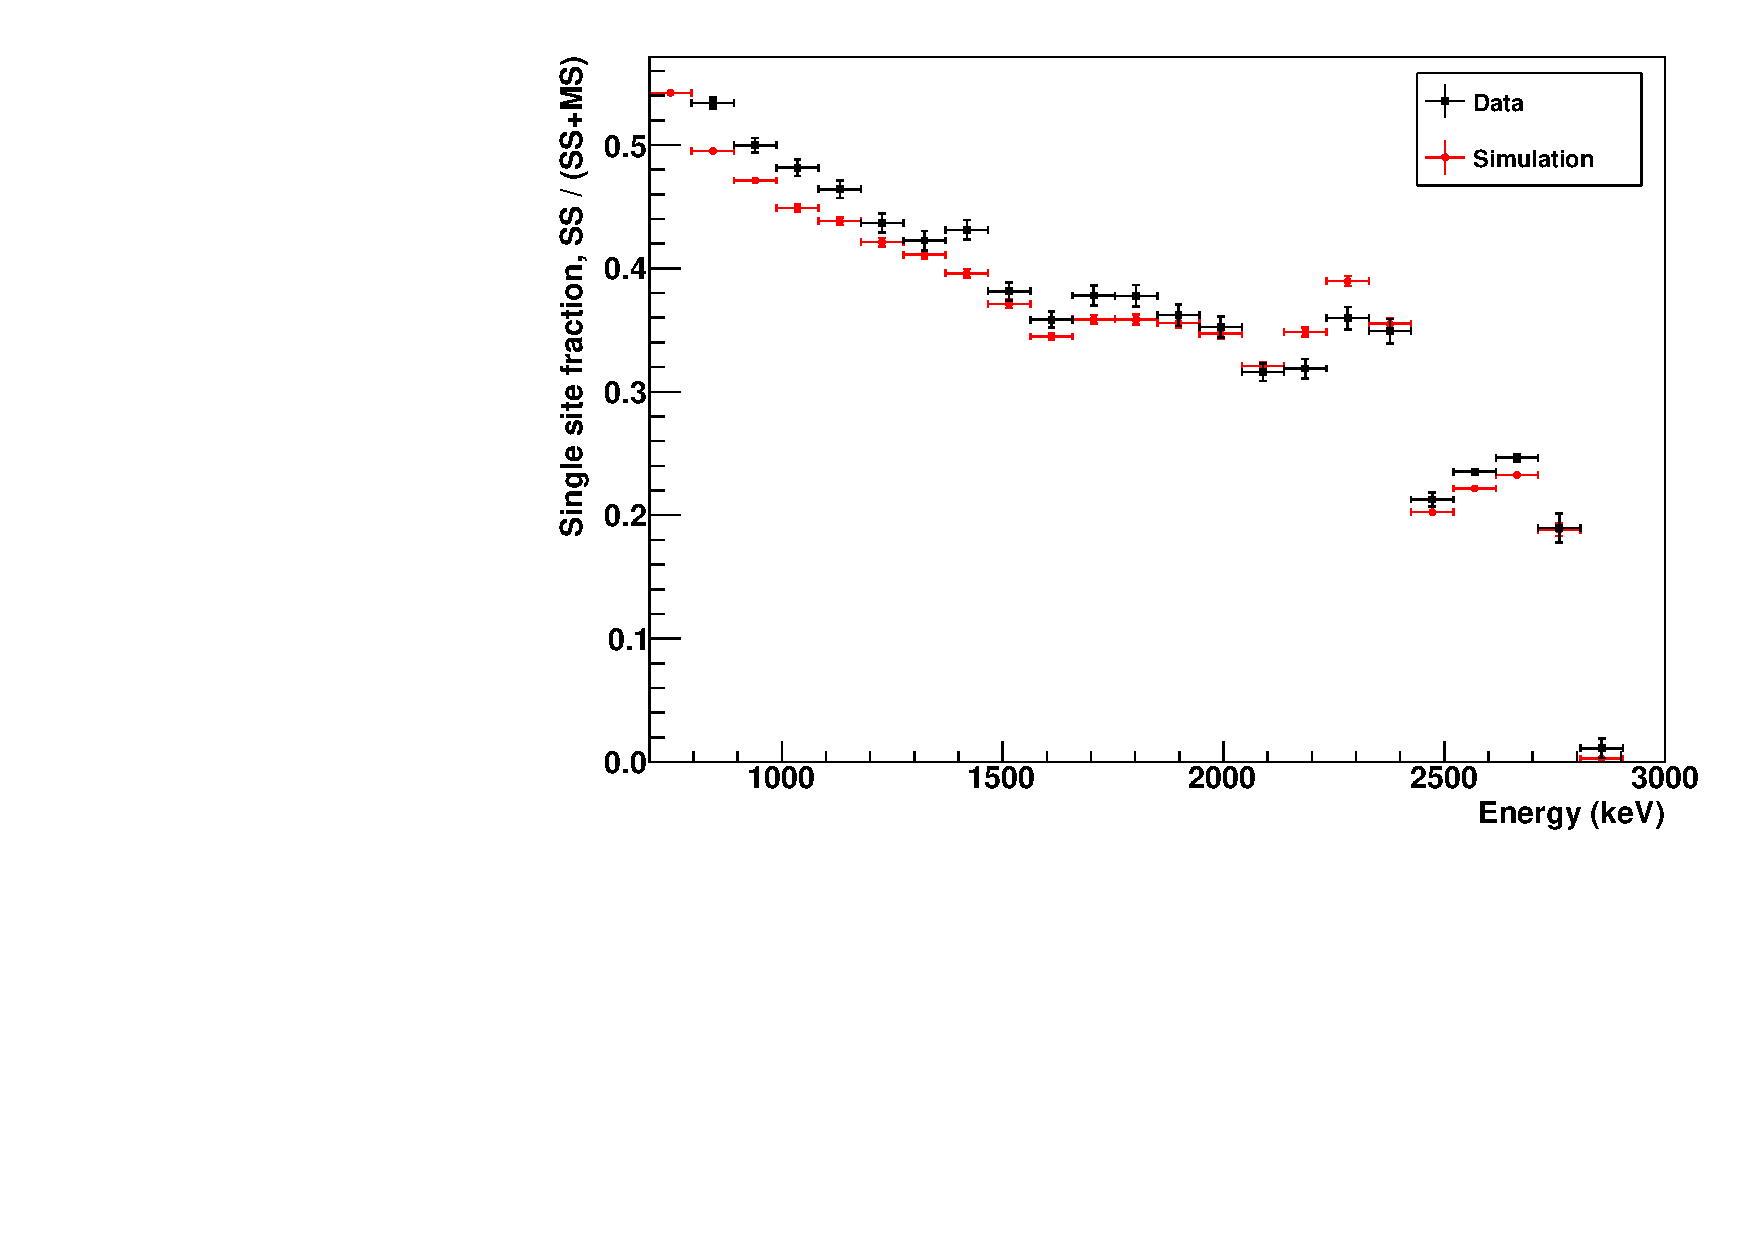
\includegraphics[width=\textwidth]{./plots/analysis_ssfrac_agreement.pdf}
	\end{subfigure}\hfill%
	\begin{subfigure}[b]{0.48\textwidth}
	\centering
	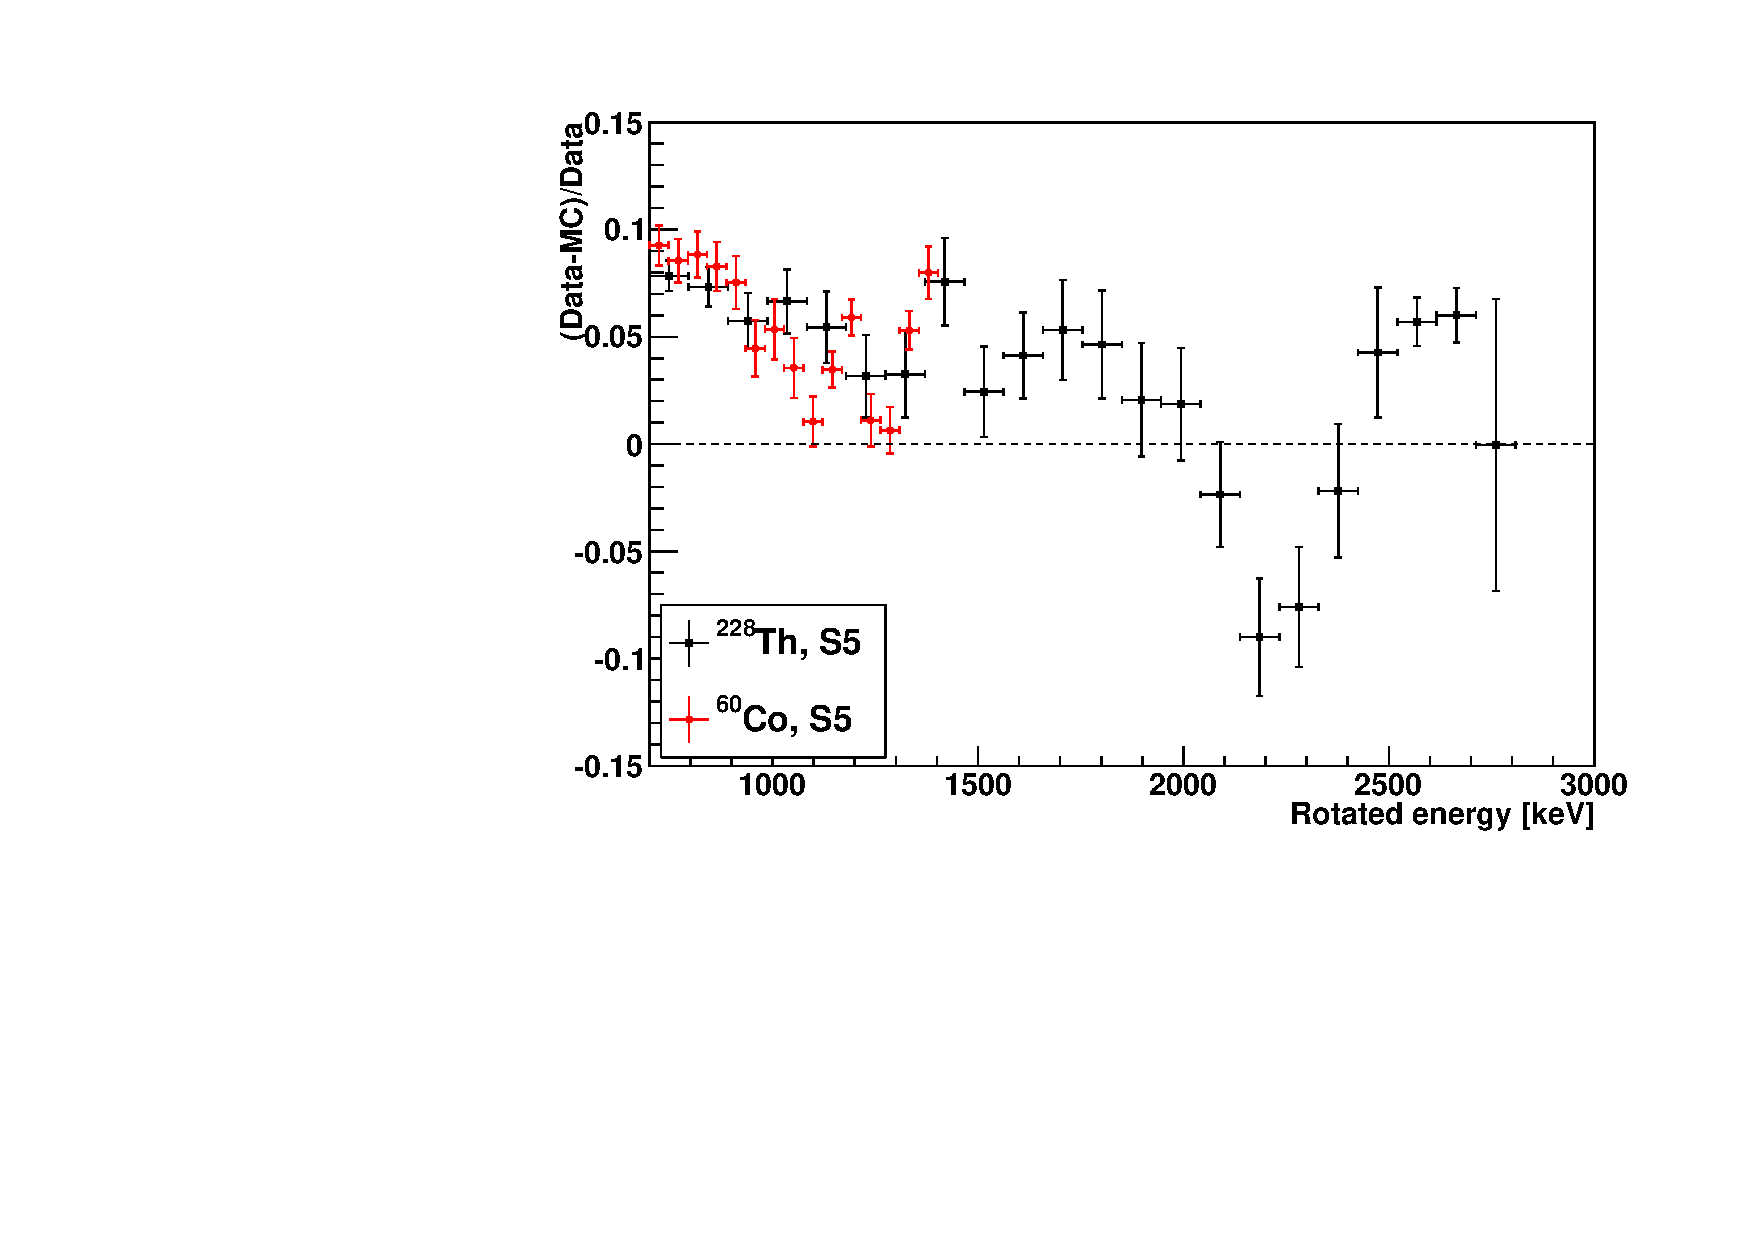
\includegraphics[width=\textwidth]{./plots/analysis_ssfrac_residuals.pdf}
	\end{subfigure}
\caption[Single site fraction agreement between simulation and data]{The left plot shows the agreement between the fraction of events that are single site in simulations and data for a \isotope{228}{Th} calibration. The right plot shows the fractional residual error between simulation and data for \isotope{60}{Co} and \isotope{228}{Th} data.}
\label{fig:analysis_ssfrac_agreement}
\end{figure}

\subsubsection{Shape Agreement}
\label{sec:analysis_shape_agreement}
One simple check is to compare the shapes of the energy and standoff distance distributions in data and simulation. \Cref{fig:analysis_shape_agreement} shows this comparison. The overall agreement in both shape and standoff distance looks reasonable. However, this agreement is not perfect. As \cref{fig:analysis_shape_agreement_ratio} shows, the simulations underpredict the fraction of single site events at low energies. This is due to a slight difference in efficiency for detecting low-energy clusters between data and simulations. This results in some events being shifted from single site to multiple site in simulations. This is not corrected for, but the systematic effect is taken into account, as described in \cref{sec:analysis_rate_uncertainty}.

\begin{figure}[htbp]
\centering
	\begin{subfigure}[c]{0.48\textwidth}
	\centering
	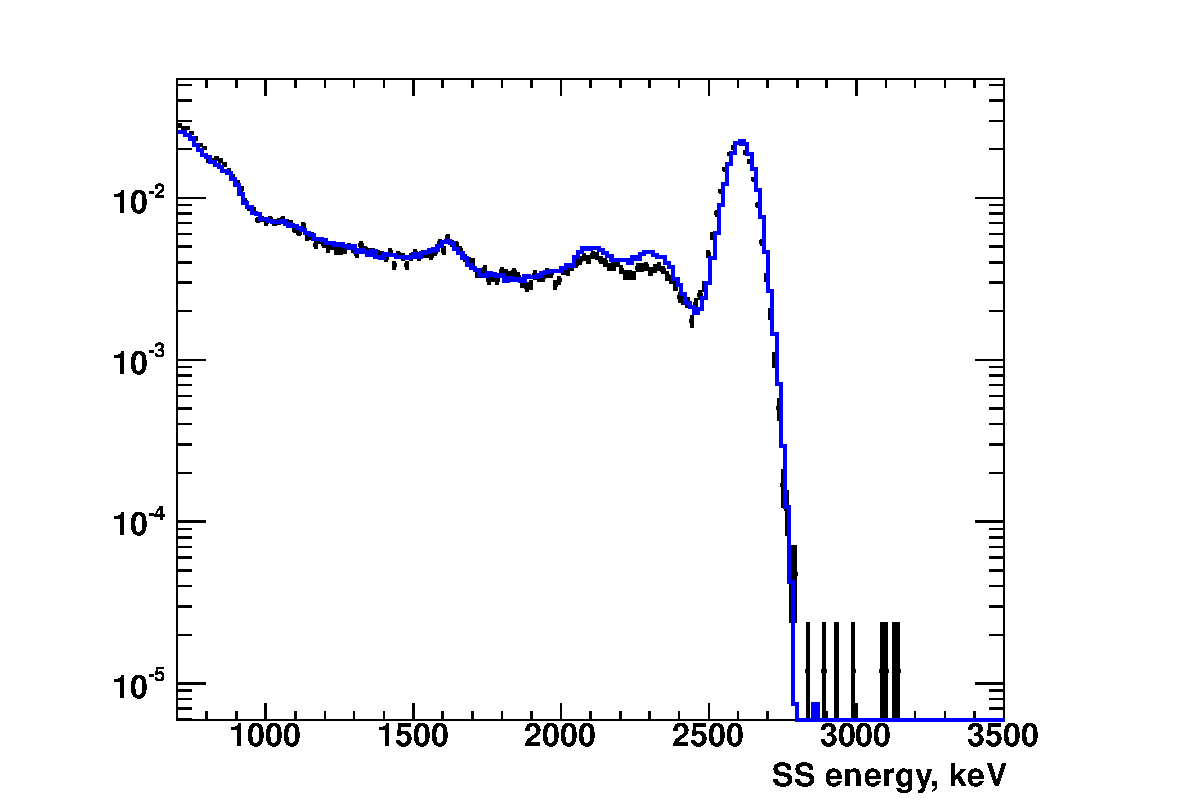
\includegraphics[trim = 1.8cm 0cm 1.5cm 1cm, clip=true, width=\textwidth]{./plots/analysis_shape_agreement_E_ThS5SSlog.pdf}
	\end{subfigure}\hfill%
	\begin{subfigure}[c]{0.48\textwidth}
	\centering
	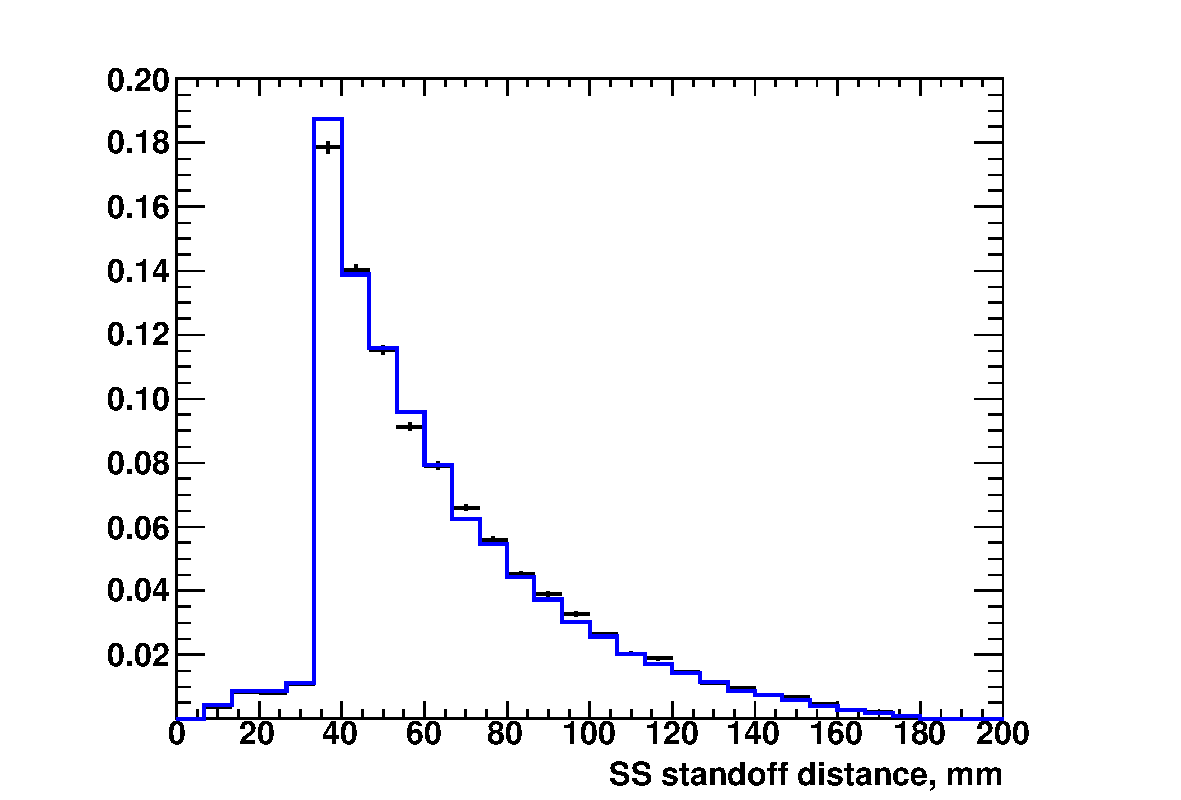
\includegraphics[trim = 1.8cm 0cm 1.5cm 1cm, clip=true, width=\textwidth]{./plots/analysis_shape_agreement_sd_ThS5SSlin.pdf}
	\end{subfigure}
	\begin{subfigure}[c]{0.48\textwidth}
	\centering
	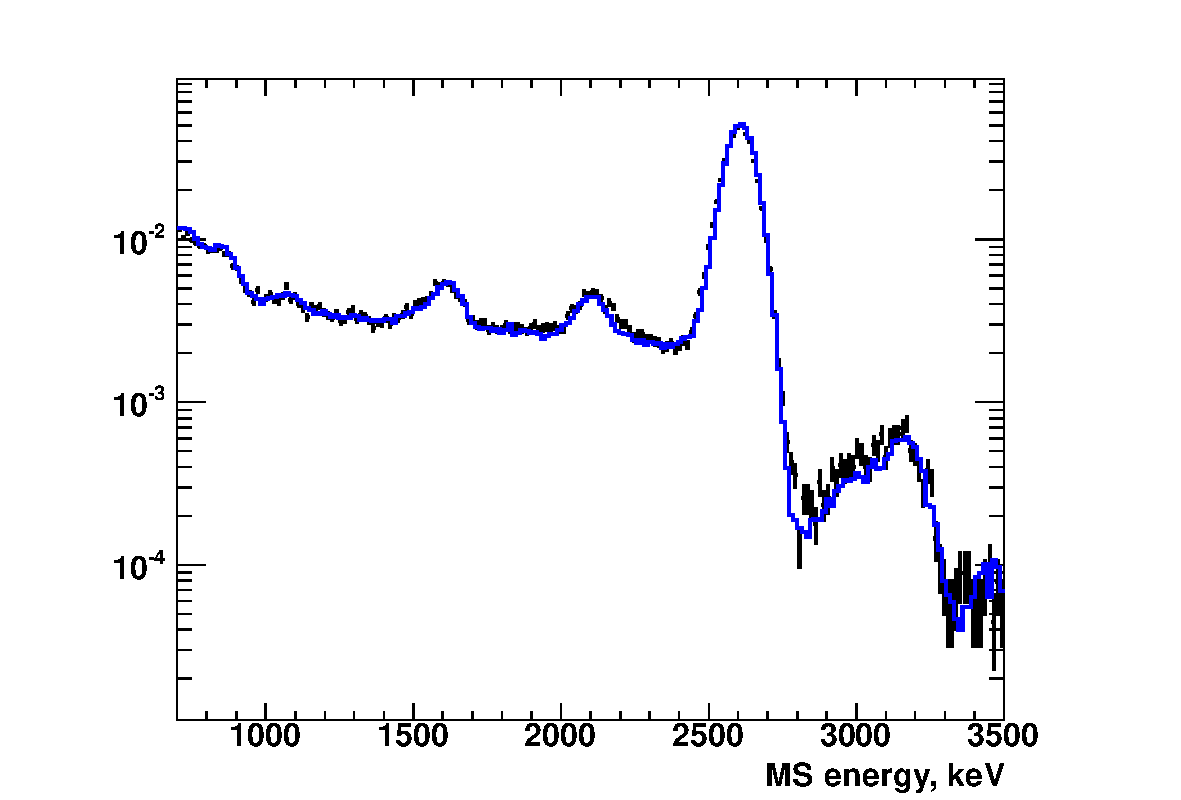
\includegraphics[trim = 1.8cm 0cm 1.5cm 1cm, clip=true, width=\textwidth]{./plots/analysis_shape_agreement_E_ThS5MSlog.pdf}
	\end{subfigure}\hfill%
	\begin{subfigure}[c]{0.48\textwidth}
	\centering
	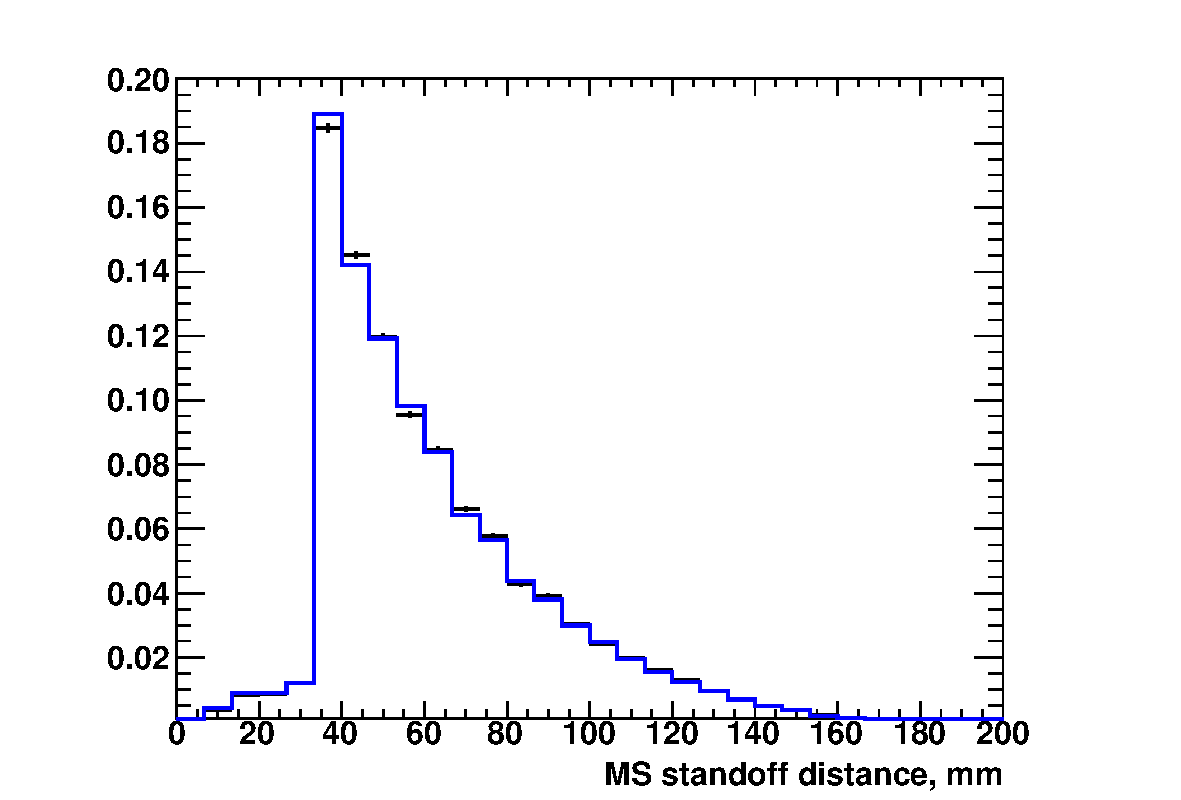
\includegraphics[trim = 1.8cm 0cm 1.5cm 1cm, clip=true, width=\textwidth]{./plots/analysis_shape_agreement_sd_ThS5MSlin.pdf}
	\end{subfigure}
\caption[Agreement between simulation and data for a \isotope{228}{Th} calibration source]{The agreement between simulations (in blue) and data (in black) for a \isotope{228}{Th} calibration source located at the cathode. The projection of the energy spectra is shown on the left, and the projection of the standoff distance distribution is shown on the right. The top row is for single site events, while the bottom row is for multiple site events.}
\label{fig:analysis_shape_agreement}
\end{figure}

\begin{figure}[htbp]
\centering
	\begin{subfigure}[c]{0.48\textwidth}
	\centering
	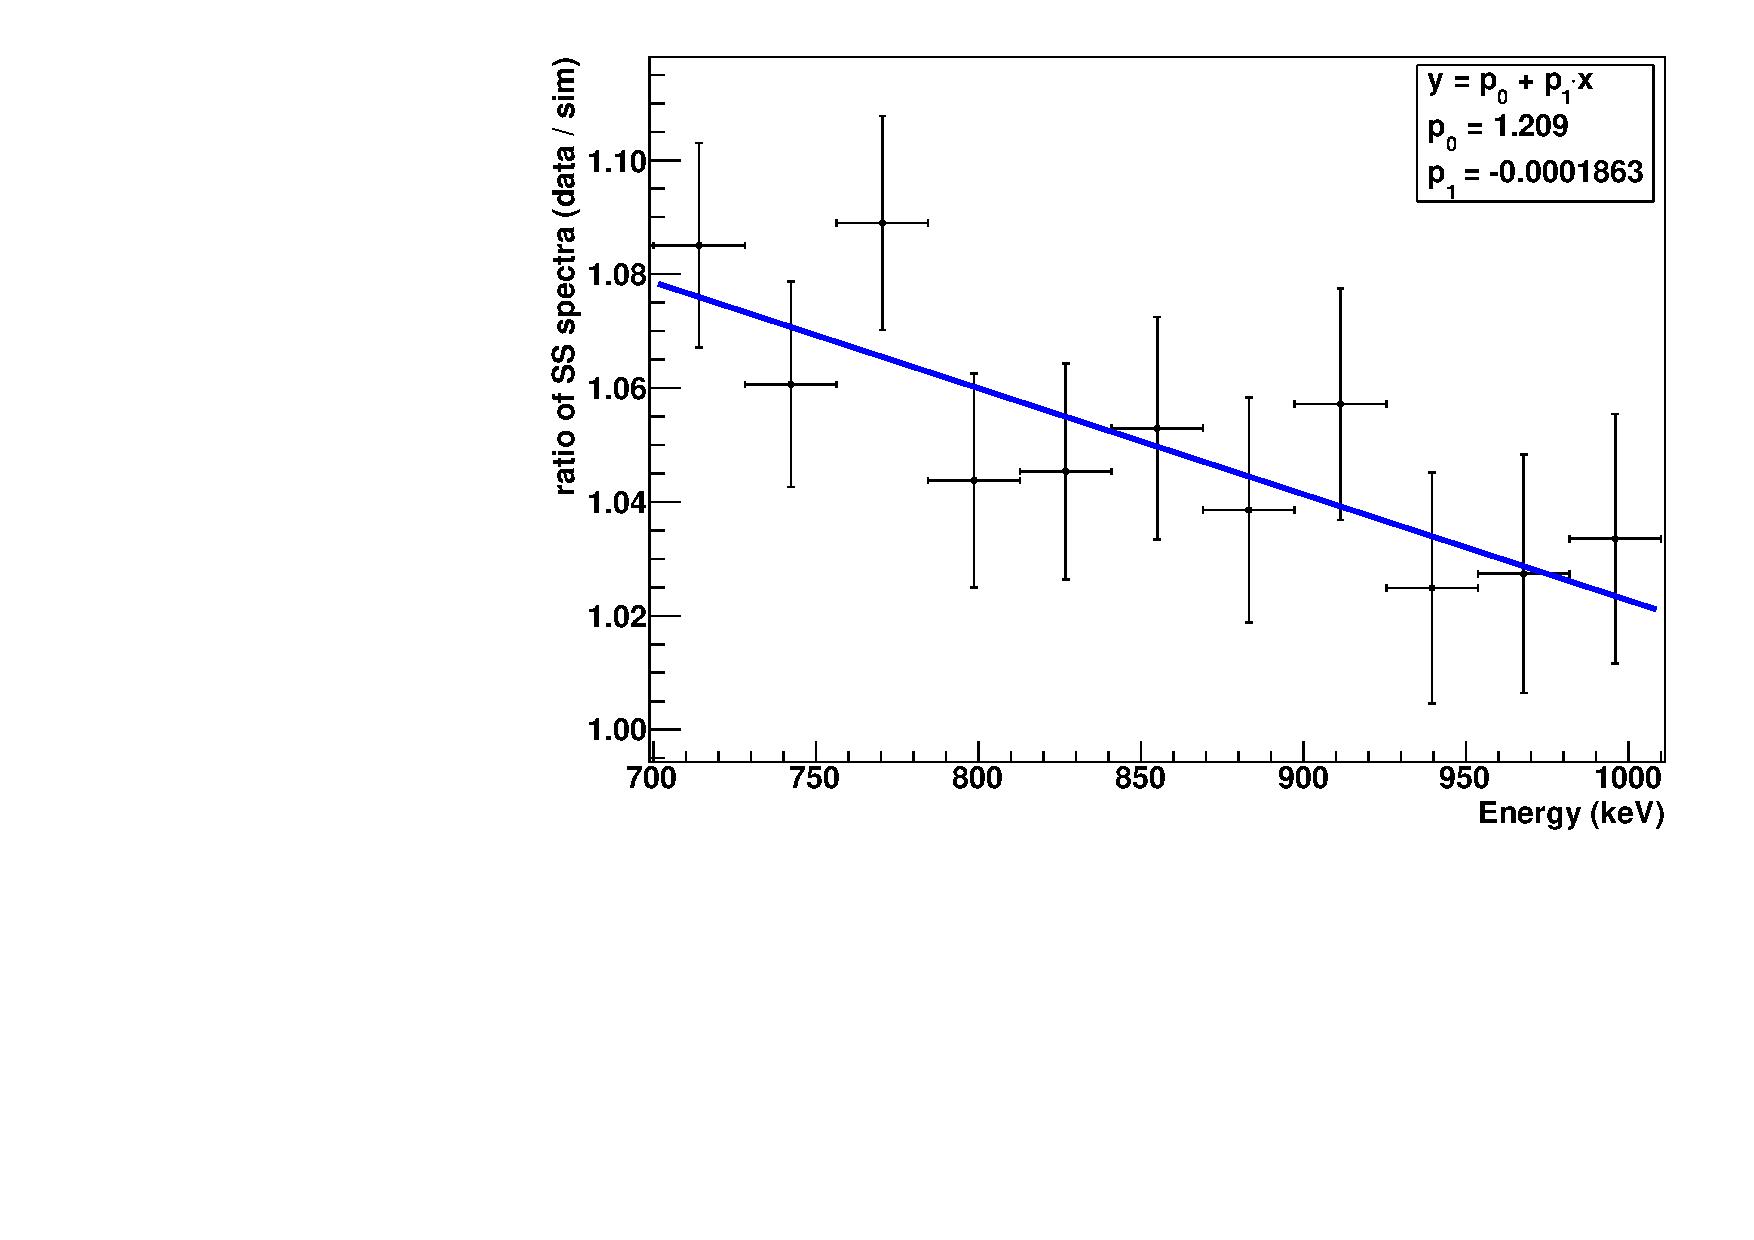
\includegraphics[width=\textwidth]{./plots/analysis_shape_agreement_ratio_ss.pdf}
	\end{subfigure}\hfill%
	\begin{subfigure}[c]{0.48\textwidth}
	\centering
	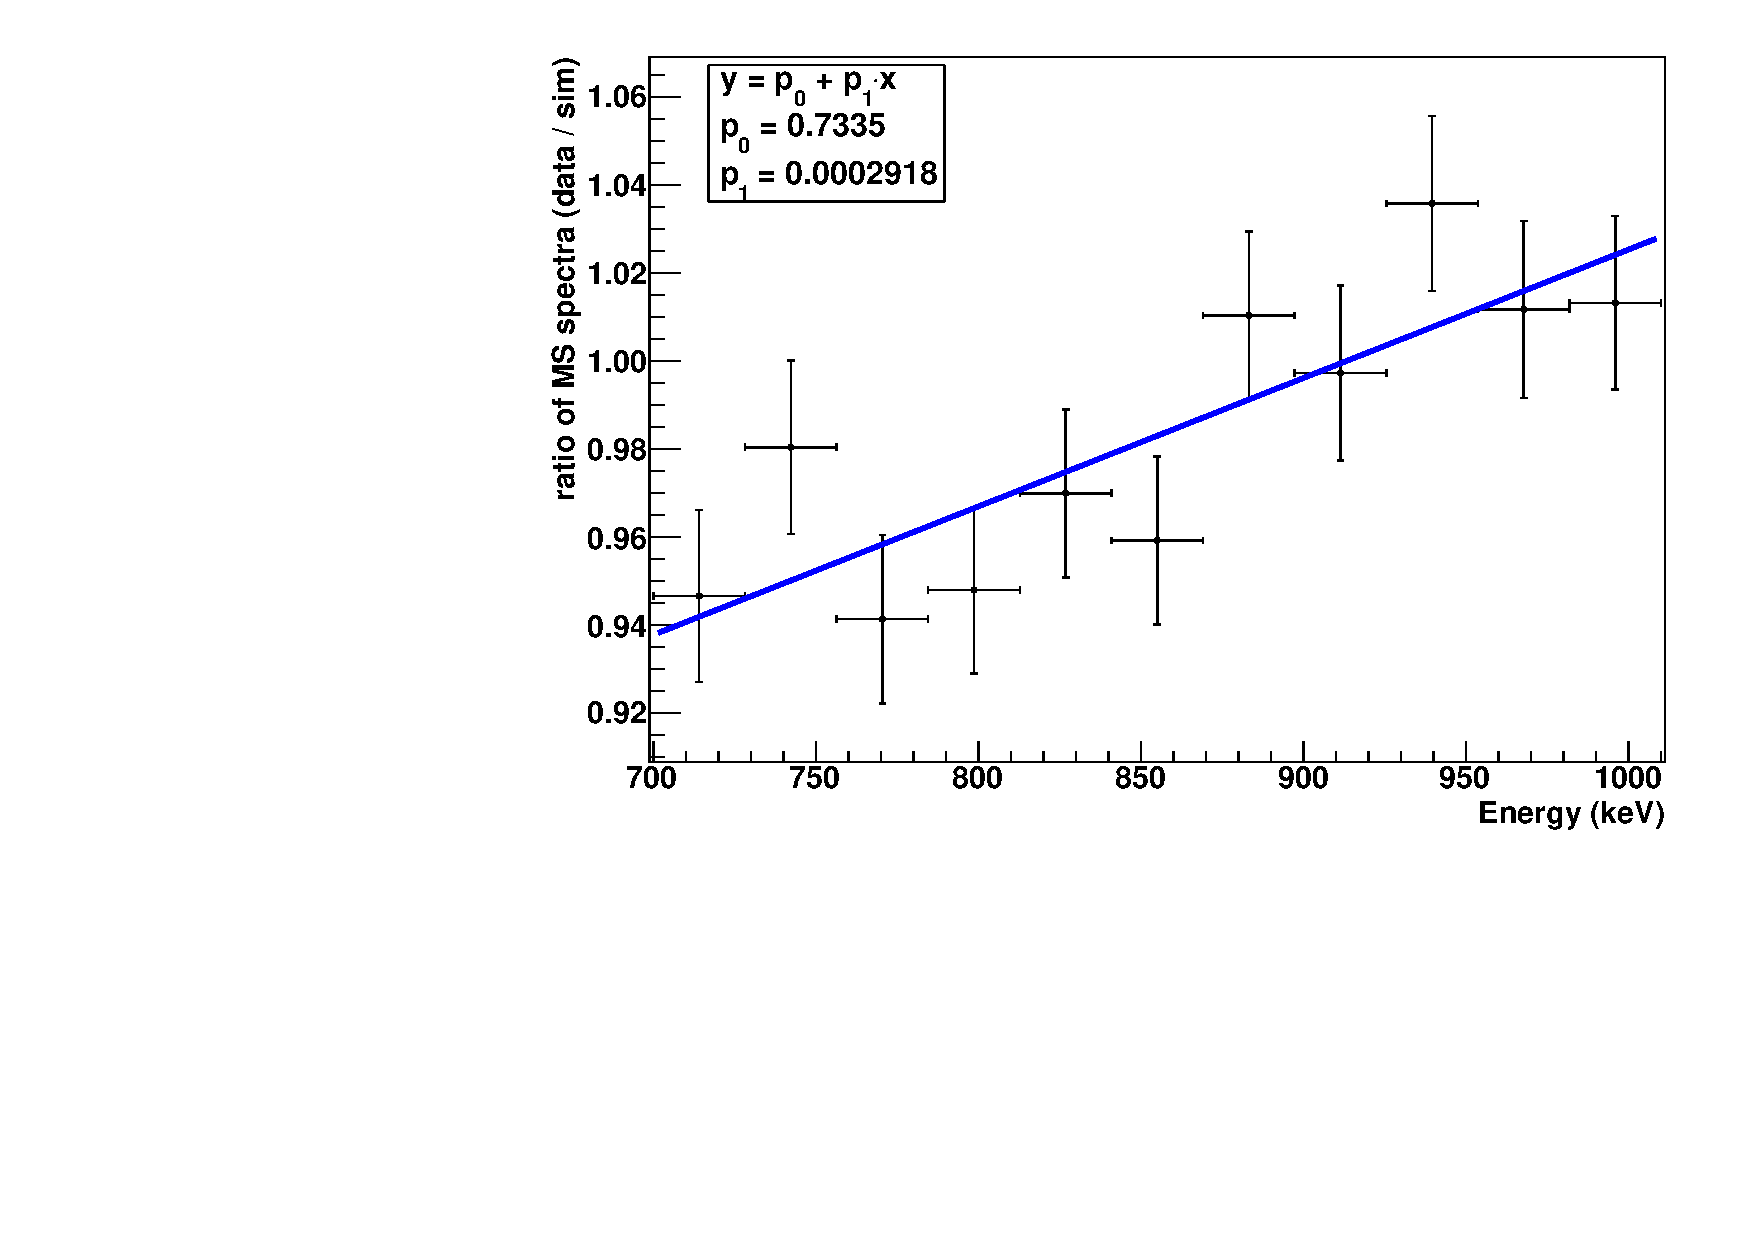
\includegraphics[width=\textwidth]{./plots/analysis_shape_agreement_ratio_ms.pdf}
	\end{subfigure}
\caption[Ratio of simulated spectra to data as a function of energy]{The ratio of the simulated energy spectrum to data for a \isotope{60}{Co} source. Single site events are shown on left, and multiple site events are shown on right. This indicates that the simulation underpredicts the fraction of single site events at low energies.}
\label{fig:analysis_shape_agreement_ratio}
\end{figure}

\subsubsection{Rate Agreement}
\label{sec:analysis_rate_agreement}
\Cref{tab:analysis_source_rate_agreement} shows the agreement between the true activity of calibration sources (based on their activity at time of manufacture and known half-life) and the rate observed using the detector and Monte Carlo simulations of the sources in order to determine efficiency. For most isotope and position combinations, the error is less than 5\%. Taking a mean (weighted by the uncertainties) of all the residuals yields (True - Estimated)/True = \SI{1.7\pm2.3}{\percent}. Contributions to this error include several effects that may not be present in non-calibration data. The source activities are only known to within 1.2\%, and the rate estimate is quite sensitive to the actual location of the source in the simulations.

\begin{table}[htbp]
\centering
\caption[Calibration source rate agreement]{Comparison of the estimated calibration source activities based on measurements in the EXO-200 detector and Monte Carlo simulations of efficiencies to their true values, based on the activity at the time of manufacture and known half life.}
\label{tab:analysis_source_rate_agreement}
\begin{tabular}{c c c c}\toprule
			&			&					&	Absolute rate agreement		\\
\multicolumn{2}{c}{Location}	&	Isotope			&	(True - Estimated)/True (\%)	\\\midrule
Anode		&	\(-z\)		&	\isotope{228}{Th}	&	\(6.2^{+0.2}_{-1.7}\)			\\
			&			&	\isotope{60}{Co}	&	\(6.0^{+0.4}_{-1.7}\)			\\
Anode		&	\(+z\)		&	\isotope{228}{Th}	&	\(-0.4^{+0.6}_{-0.5}\)			\\
			&			&	\isotope{60}{Co}	&	\(2.3^{+0.5}_{-0.8}\)			\\
Cathode		&	\(+x\)		&	\isotope{228}{Th}	&	\(3.6^{+0.7}_{-1.4}\)			\\
			&			&	\isotope{60}{Co}	&	\(0.9^{+1.0}_{-1.5}\)			\\
Cathode		&	\(+y\)		&	\isotope{228}{Th}	&	\(4.5^{+3.3}_{-3.2}\)			\\
			&			&	\isotope{60}{Co}	&	\(5.1^{+3.2}_{4.0}\)			\\\bottomrule
\end{tabular}
\end{table}

\section{Systematic Uncertainties}
\subsection{Rate Uncertainty}
\label{sec:analysis_rate_uncertainty}
While the rate agreement with calibration sources provides an estimate of the accuracy to which the detector can measure decay rates, it is possible to estimate this uncertainty directly. \Cref{tab:analysis_normalization_uncertainty} summarizes these estimates.

\begin{table}[tbp]
\centering
\caption[Contributions to systematic uncertainty]{Estimated contributions to the uncertainty for rates measured in the detector. Some contributions are energy independent, and so are calculated separately for the different modes.}
\label{tab:analysis_normalization_uncertainty}
\begin{tabular}{p{0.45\textwidth} c c c c c}\toprule
			&	\multicolumn{5}{c}{Contribution to rate uncertainty (\%)}				\\
Component	&	\twonu{}	&	\multicolumn{4}{c}{\(0\nu\beta\beta\chi^0(\chi^0)\)}		\\
			&			&	\(n = 1\)	&	\(n = 2\)	&	\(n = 3\)	&	\(n = 7\)	\\
Tagged noise in coincidence with physics events		&	\multicolumn{5}{c}{\(1\times10^{-3}\)}		\\
Physics events mis-identified as noise				&	\multicolumn{5}{c}{\(<0.06\)}				\\
%Falsely finding a second scintillation signal			&	\multicolumn{5}{c}{\(4.0\)}				\\
Falsely finding a second scintillation signal			&	2.2	&	1.6	&	1.9	&	2.1	&	2.1	\\
Fiducial volume due to bias in position reconstruction	&	\multicolumn{5}{c}{\(1.73\)}				\\
Fiducial volume due to position reconstruction resolution	&	\multicolumn{5}{c}{\(0.36\)}				\\
Energy calibration and resolution uncertainty			&	0.36	&	0.04	&	0.09	&	0.36	&	0.56	\\
Energy scale difference between \(\beta\) and \(\gamma\)	&	0.17	&	0.09	&	0.20	&	0.37	&	1.40	\\
Induction tagging								&	\(<0.2\)&	\(<0.66\)	&	\(<0.44\)	&	\(<0.21\)	&	\(<0.28\)	\\
Triggering efficiency	(above \SI{700}{\keV})			&	\multicolumn{5}{c}{\(\approx 0\)}			\\
Signal-finding efficiency (above \SI{700}{\keV})		&	\multicolumn{5}{c}{\(\approx 0\)}			\\
Clustering efficiency								&	\multicolumn{5}{c}{\(2.0\)}	\\
Shape distortion in \SIrange{700}{1000}{\keV}			&	\multicolumn{5}{c}{0.75}					\\
Xenon isotopic fraction							&	\multicolumn{5}{c}{0.6}					\\\midrule
\textbf{Total}									&\textbf{3.6}&\textbf{3.3}&\textbf{3.4}&\textbf{3.5}&\textbf{3.8}\\\bottomrule
%\textbf{Total}									&\textbf{2.85}&\textbf{2.90}&\textbf{4.86}&\textbf{2.85}&\textbf{3.32}\\\bottomrule
\end{tabular}
\end{table}

Noise events (as identified by the noise tagger) may occur in coincidence with real events. By simply comparing the \SI{11}{\milli\Hz} rate for real events and the \SI{75}{\milli\Hz} rates for noise events, the probability for one to occur in the \SI{1024}{\micro\s} following a trigger by the other, thus removing a real event from the data set, is \num{8.9e-5}. Likewise, hand-scanning events tagged as noise puts an upper limit on the rate at which legitimate physics events are tagged as noise at \(< 5.8e-4\).

Noise fluctuations in the APD waveforms might be reconstructed as scintillation signals. These events would be rejected by the requirement that events have only one scintillation signal. About \SI{0.75}{\percent} of events in real data are removed by this cut, while \about{}\SI{4}{\percent} of events in Monte Carlo simulations of \twonu{} events are removed. Since the real data consists chiefly of \twonu{} events, and since there should be some genuine coincides in that data, too many simulated events are failing this cut. This is attributed to the matched filter signal finding technique being optimized to work on APD signals with real noise, when the Monte Carlo simulations only have simulated white noise. When determining the efficiency for double beta events to survive all cuts, all of these false coincidences could survive the other cuts, or all could fail. Therefore, the efficiency used when computing a half life is taken midway between these extremes, and half the difference between the extremes is propagated as a systematic error.

Monte Carlo simulations of \twonu{} events suggest that the RMS error on the \(u\), \(v\), and \(x\) coordinates that are used to define hexagonal cross-section of the fiducial volume are \SI{2.4}{\mm}, \SI{1.2}{\mm}, and \SI{2.7}{\mm}, respectively. The error on the \(z\) coordinate due to slight deviations from a uniform electric field is \SI{0.42}{\mm}. Meanwhile, studies of events that occur on the cathode and so create signals in both TPCs suggest there might be a \SI{1.5}{\mm} offset in \(u\) and \(v\) and a \SI{0.5}{\mm} offset in \(z\) between the two TPCs. These might be physical, due to slight asymmetries in the construction, but are taken as systematic errors. Combining these uncertainties gives a total \SI{1.73}{\percent} uncertainty on the fiducial volume. Furthermore, position resolution considerations mean some events inside the fiducial volume can be reconstructed outside, and vice versa. Assuming uniform events, this should be a \(+\SI{0.36}{\percent}\) effect on the rate. It is, however, taken as a symmetric systematic error and is not corrected.

The energy range used for the fit has a \SI{700}{\keV} lower limit, since the trigger and reconstruction are known to be \SI{100}{\percent} efficient above that energy. Uncertainty on the energy calibration means some events might mistakenly be left out of the data set used in the fit. At \SI{700}{\keV}, the energy uncertainty is \SI{2.5}{\keV}. Comparing the number of events in the spectrum within \SI{700\pm2.5}{\keV} to the total number of events above \SI{700}{\keV} gives an estimate of this uncertainty's effect. Since it depends on the shape of the spectrum under consideration, it is computed separately for the different double beta decay modes.

The \SI{2615}{\keV} \(\gamma\) ray from \isotope{228}{Th} may produce an electron-positron pair that should be topologically similar to a double beta decay event. Using the \SI{511}{\keV} gamma rays produced by positron annihilation as a tag gives a very clean sample of these events. Studying the ionization of the electron-positron pair suggests that there may be a systematic shift in the energy scale for \(\beta\) events compared to \(\gamma\) events. \Cref{fig:analysis_beta_scale} shows an example. Propagating this difference through all rotations and calibrations suggests that \(\beta\) events should have their energies multiplied by a factor \num{1.0115\pm0.0052} in order to match the calibration from \(\gamma\) events. Meanwhile, generating PDFs for different energy scale differences and determining which best fit the data (as described below) suggests the best value for this factor is \num{1.001\pm0.003}. For \twonu{} the effect on the rate uncertainty is done by performing the fit at \num{1.001\pm0.011} and observing the change in the number of events found. For the Majoron-emitting modes, this is instead determined similarly to the energy scale uncertainty, by seeing how many events pass above and below the \SI{700}{\keV} threshold as the factor is varied between \num{1.001\pm0.011}.

\begin{figure}[tbp]
\centering
	\begin{subfigure}[c]{0.48\textwidth}
	\centering
	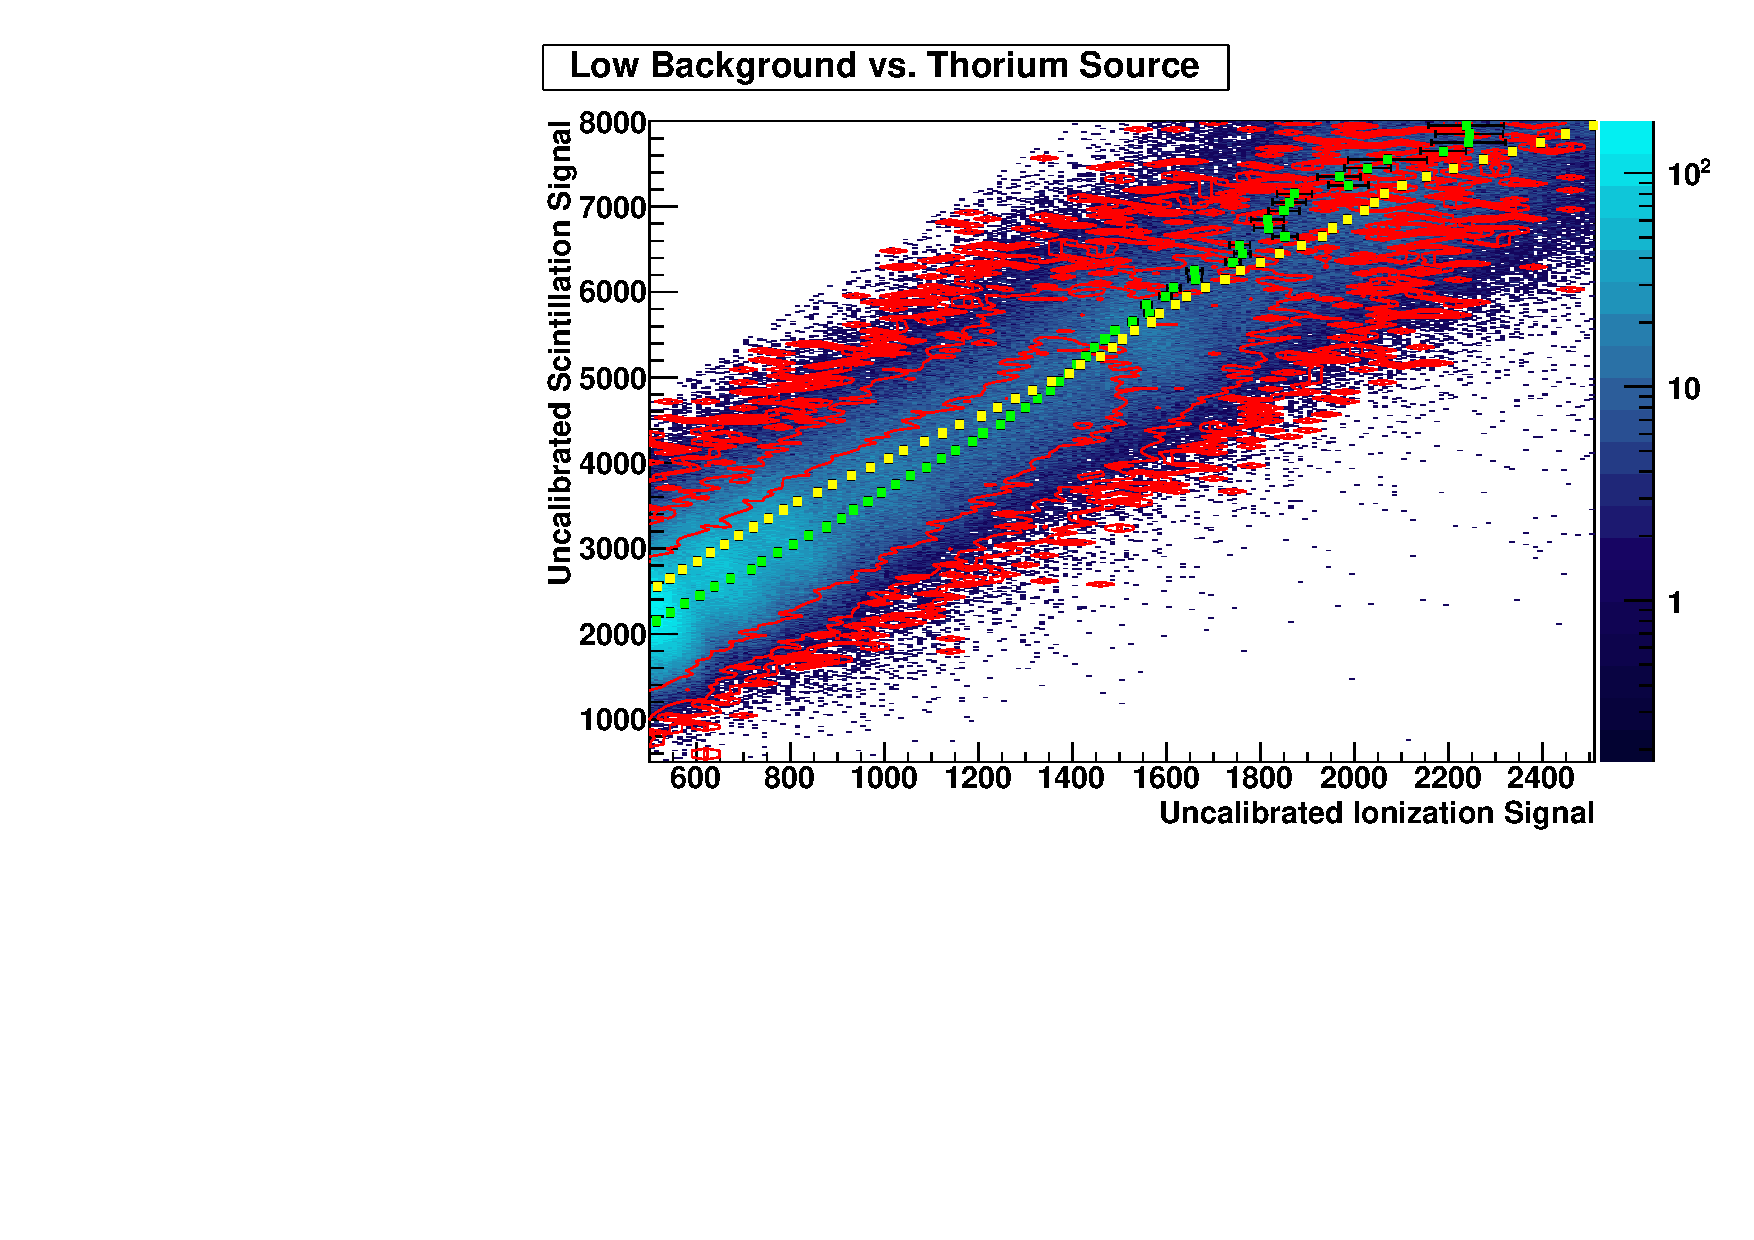
\includegraphics[width=\textwidth]{./plots/analysis_beta_gamma_comparison.pdf}
	\end{subfigure}\hfill%
	\begin{subfigure}[c]{0.48\textwidth}
	\centering
	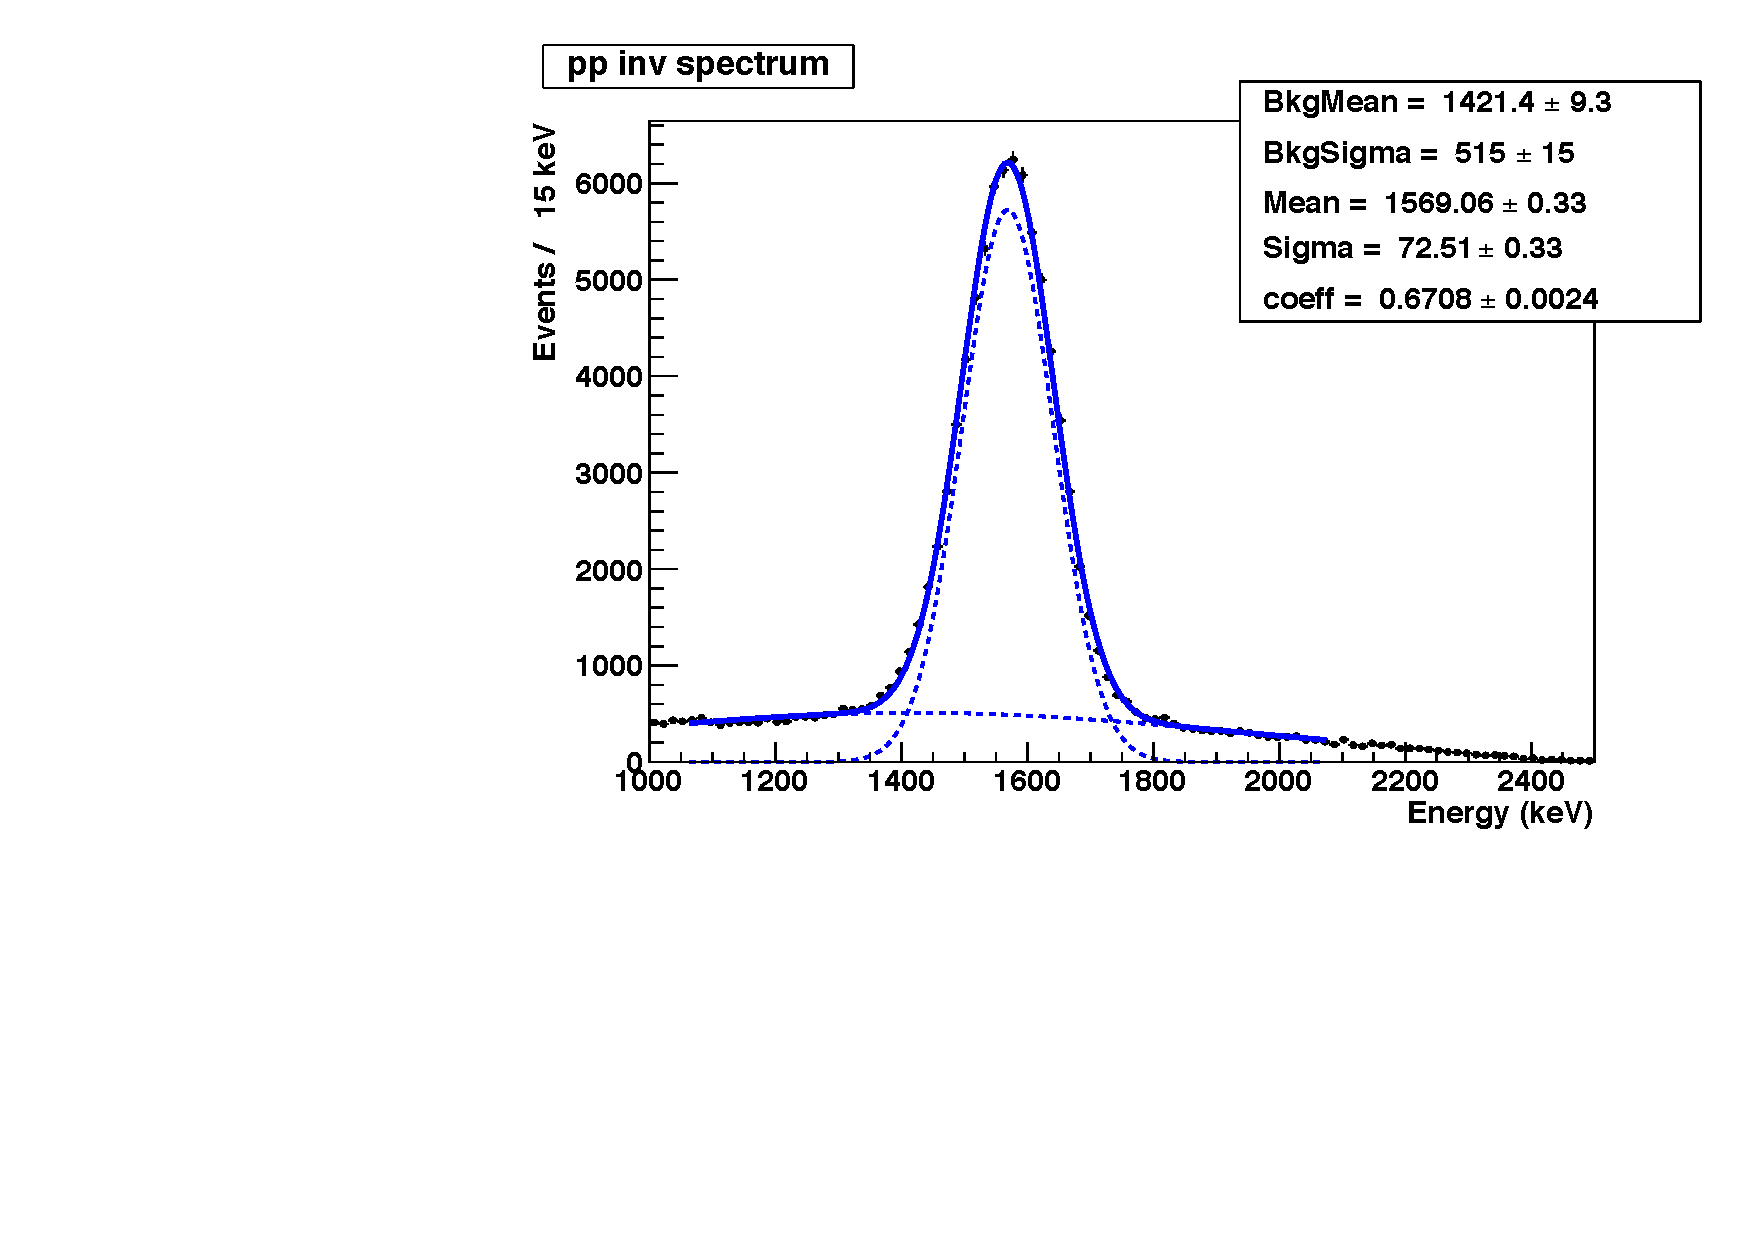
\includegraphics[width=\textwidth]{./plots/analysis_calibrated_pp_peak.pdf}
	\end{subfigure}
	\caption[Evidence that \(\beta\) and \(\gamma\) events might have different energy scales]{(Left) A comparison of the mean ionization signal for a given amount of scintillation in low background (green dots and red contours) data, compared to that for thorium calibration (yellow dots and blue shading). The low background data, consisting chiefly of \(\beta\) events, shows larger ionization signals than the thorium data, consisting chiefly of \(\gamma\) events. (Right) After applying the energy calibration (based on \(\gamma\) ray emitting sources) the pair production peak of a \SI{2615}{\keV}, which is a \(\beta\) type event, reconstructs below its expected \SI{1593}{\keV} energy.}
\label{fig:analysis_beta_scale}
\end{figure}

The clustering efficiency uncertainty is determined by comparing the number of events that pass all cuts except the one requiring all charge bundles to be fully clustered to the number of events that pass all cuts. This is done in both simulations of \twonu{} and real data. Since there are backgrounds in the real data which may have different rates, background subtraction is done using the best fit to the data (described below in \cref{sec:analysis_twonu_measurement}. The difference between background-subtracted data and simulation is energy dependent, and so integrating over the \twonu{} spectrum gives the uncertainty listed in \cref{tab:analysis_source_rate_agreement}.

Simulations predict a shape for the spectrum between about \SIrange{700}{1000}{\keV} that disagrees with calibration data. This shape error is similar for \isotope{60}{Co} and \isotope{228}{Th}, and can be parameterized as shown in \cref{fig:analysis_shape_agreement_ratio}. This could be used as a correction, but instead it is taken as a systematic uncertainty. All PDFs are ``skewed'' to effectively undo this error, and then used to generate toy Monte Carlo simulations with similar amounts of signal and background as in the Run2a data. The resulting toy sets are then fit with the original, unskewed PDFs. The result is that the number of \twonu{} events returned by the fit is systematically \SI{0.75}{\percent} higher than the number generated in the simulation. Therefore, this is the contribution to the \twonu{} rate uncertainty. The Majoron-emitting modes with spectral indices 1, 2, and 3 have less of their spectrum at these low energies, and so using the \twonu{} uncertainty is a conservative estimate. For spectral index 7, the sign of the distortion would tend to cause the number of these decays to fit to higher than their true values. Thus, if a limit is obtained for spectral index 7, it will still be conservative, even using the \twonu{} uncertainty.

Finally, there is uncertainty as to precisely how many \xenon{136} atoms are in the fiducial volume. The uncertainty on the enrichment fraction of \SI{80.6\pm0.2}{\percent}, for example, contributes a \SI{0.3}{\percent} uncertainty. Isotope fractionation between the liquid and gas phases is small, contributing less that \SI{1e-3}{\percent} uncertainty. Some natural xenon from a commissioning run may have remained dissolved in plastic TPC parts, possibly diluting \xenon{136} by \SI{0.04}{\percent}. The dominant contribution comes from uncertainty about the density. Allowing for a \SI{\pm2.5}{\percent} uncertainty in xenon temperature changes the density by \SI{\pm0.6}{\percent}.

\subsection{Other PDFs}
\subsubsection{Other Backgrounds}
A number of radioactive isotopes are only simulated in the TPC vessel. However, since the cryostat, for example, is made of the same copper, it seems reasonable to include simulations for it as well. And, likewise, other sources of background can be imagined. In the Run2a data set, however, there are not enough events to statistically distinguish backgrounds in different components. \Cref{fig:analysis_degenerate_uranium_spectra} shows projections of the energy and standoff distance spectra for \isotope{238}{U} in the TPC vessel and the inner cryostat, normalized to the number of \isotope{238}{U} decays returned by the fit. Statistical errors are shown.
 
\begin{figure}[tbp]
\centering
\begin{subfigure}[c]{\textwidth}
	\centering
	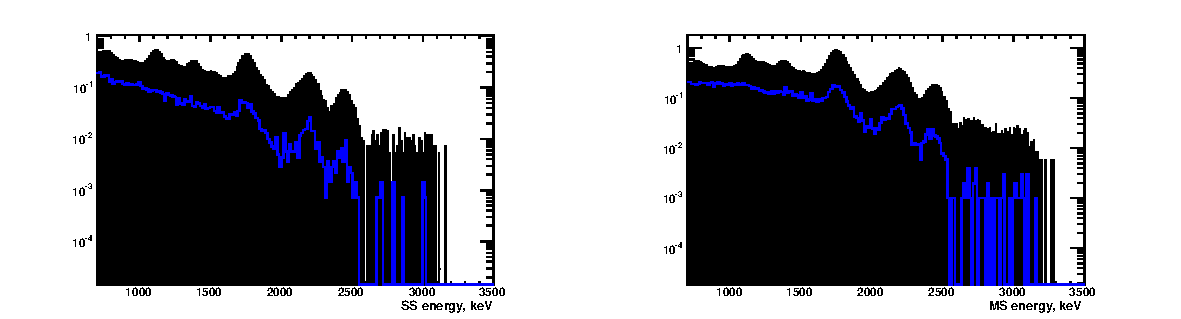
\includegraphics[width=\textwidth]{./plots/analysis_degenerate_uranium_spectra_e.pdf}
\end{subfigure}
\begin{subfigure}[c]{\textwidth}
	\centering
	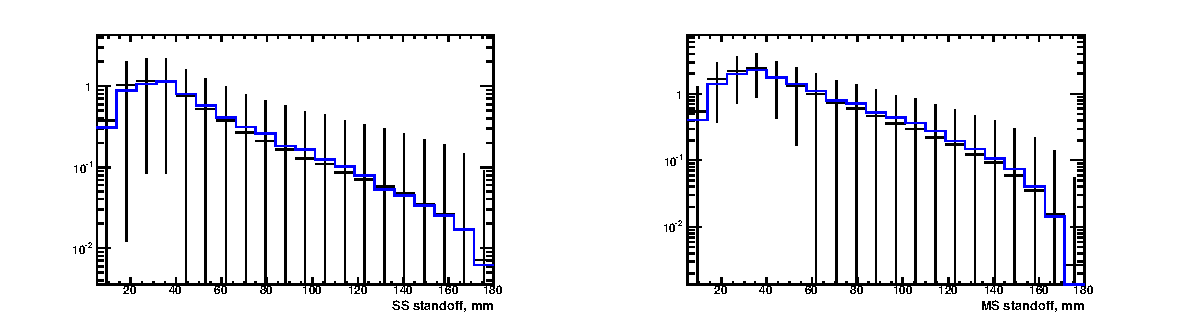
\includegraphics[width=\textwidth]{./plots/analysis_degenerate_uranium_spectra_s.pdf}
\end{subfigure}
\caption[Lack of statistical power to distinguish the source of uranium backgrounds]{Projections of the energy (top) and standoff distance (bottom) spectra for \isotope{238}{U} in the TPC vessel (black points) and in the inner cryostat (blue line). Single site events are on the left, and multiple site events are on the right. The error bars are statistical, normalized to the number of \isotope{238}{U} decays returned by the fit. The two spectra are statistically indistinguishable without more data.}
\label{fig:analysis_degenerate_uranium_spectra}
\end{figure}

Neutron-induced backgrounds are difficult to model. The most likely candidate background, due the large volume of HFE and its close proximity to the TPC, is the \SI{2.2}{\MeV} \(\gamma\) ray produced by neutron capture on hydrogen. Using the muon flux measured in \cref{ch:muons} and FLUKA \cite{Ferrari:2005zk} simulations of the EXO-200 detector, a conservative estimate for the number of \SI{2.2}{\MeV} \(\gamma\) rays seen in the data is roughly 40, split evenly between the single-site and multiple-site spectra. Attempting to include the \(\gamma\) line in the fit (described below) yields a best fit of 23 events, but not significant at even the \(1\sigma\) level. Therefore, this potential background is not included in the fit, and will only be a small effect if present.

\subsubsection{Missing wire channel}
For a period of roughly 1 month, the data collected from the detector did not include one collection wire (numbered channel 16). In order to determine the effect of this period on the overall spectrum PDFs were constructed for data with and without this channel included and combined, weighted by their fraction of total live time in Run2a. The period with the missing channel constitutes \SI{5.2}{\percent} of the total time. These weighted PDFs were compared with the default PDFs with all channels working. The reduced \(\chi^2\) of 0.1 shows the spectra are quite compatible. A Kolomgorov-Smirnov test reports \SI{89.7}{\percent} probability for compatibility. Therefore, the default spectra are used, since they closely match the weighted spectra, which are more complicated to produce.

\begin{figure}[htbp]
\centering
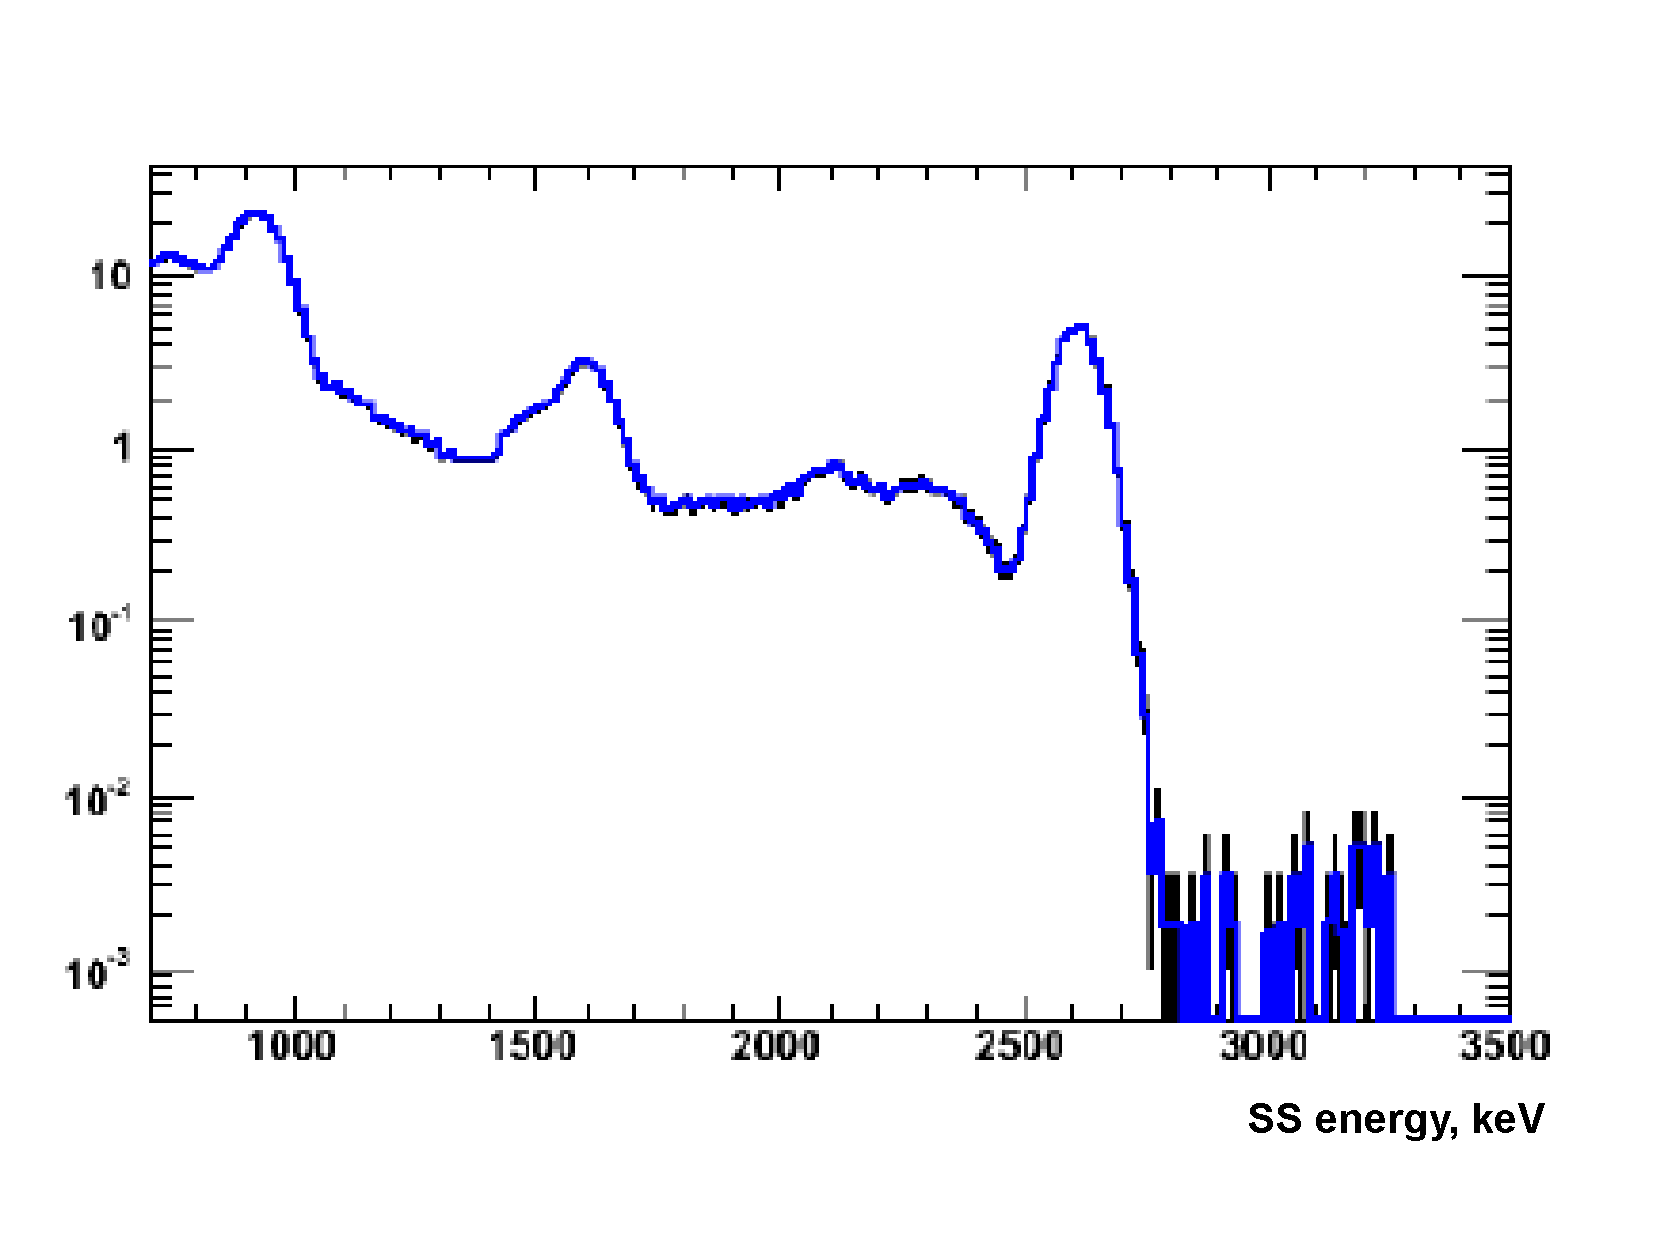
\includegraphics[width=0.7\textwidth]{./plots/analysis_missing_channel16_comparison.pdf}
\caption[Comparison of default PDF to PDF with missing channel]{A comparison of the default PDF for \isotope{232}{Th} in the TPC vessel (black) to one that accounts for the time period in which one collection wire was not taking data (blue). The two spectra are quite compatible, with a reduced \(\chi^2\) of 0.1, and a Kolmogorov-Smirnov test indicating \SI{89.7}{\percent} probability for compatibility.}
\label{fig:analysis_missing_channel16_comparison}
\end{figure}

\section{Maximum Likelihood Method}
\subsection{Theory}
\label{sec:analysis_ml_theory}
When attempting to measure a decay rate (as for double beta decay), the parameter measured is the number of decays in a given amount of time. This is complicated by the presence of backgrounds. Ultimately, the collected data is a combination of many backgrounds and possibly signals, each parameterized by a number of decays. A maximum likelihood analysis provides a way to estimate these parameters and their uncertainties, or to place limits on the parameters.

In a maximum likelihood analysis, first a likelihood function \(\mathcal{L}\) is established:
\begin{equation}
\mathcal{L} = \prod_i f(x_i|\boldsymbol{\theta})
\end{equation}
where \(f(x_i|\boldsymbol{\theta})\) is a probability density function with parameters \(\boldsymbol{\theta}\) for the observed data \(x_i\). The data are fixed, while the parameters can vary. Thus \(\mathcal{L}\) is the likelihood that the parameters \(\boldsymbol{\theta}\) describe the probability distribution underlying the data.

Finding the set of parameters that best describe the data, then, becomes a matter of maximizing \(\mathcal{L}\). In practice, since \(\mathcal{L}\) is always less than one and can be quite small for some choices of parameters, it is easier to work with the negative logarithm of the likelihood function, or ``negative log-likelihood''. Maximizing \(\mathcal{L}\) becomes minimizing the negative log-likelihood. This can be done analytically for simple cases, but for most problems numerical minimization package such as MINUIT \cite{James:1975kx} is used.

The maximum likelihood method can be used to construct confidence intervals. Define
\begin{equation}
\lambda({\theta_0}) = \ln \mathcal{L}_{max}(\boldsymbol{\theta}) - \ln \mathcal{L}_{max}(\theta_0, \boldsymbol{\theta}')
\end{equation}
where \(\mathcal{L}_{max}(\boldsymbol{\theta})\) denotes the likelihood maximized over all parameters. \(\mathcal{L}_{max}(\theta_0, \boldsymbol{\theta}')\) denotes the likelihood maximized over all parameters except for \(\theta_0\), which is held fixed. Wilks' theorem \cite{Wilks:1938uq} says that the distribution of \(\lambda\) can be approximated by
\begin{equation}
2\lambda(\theta_0) \sim \chi^2_{\text{dim}(\theta_0)}
\label{eq:analysis_nll_distribution}
\end{equation}
where \(\chi^2_{\text{dim}(\theta_0)}\) is the \(\chi^2\) distribution with degrees of freedom equal to the dimensionality of \(\theta_0\). Then the \(\alpha\%\) level confidence interval on \(\theta_0\) is bounded by \(\theta_0^-\) and \(\theta_0^+\) such that \(2\lambda(\theta_0^\pm)\) is equal to the \(\chi^2\) quantile for \(\text{dim}(\theta_0)\) degrees of freedom at the \(\alpha\%\) level.

It may happen, however, that when measuring physical quantities, the best fit parameters or confidence intervals may be unphysical. A radioactive isotope can not have a negative number of decays, for example. Rolke et al. \cite{Rolke:2005uq} propose a method to extract limits in these situations. Suppose that \(\theta_0\) cannot be negative, but the best fit has \(\theta_0 < 0\). Their method of bounded likelihood sets \(\theta_0 = 0\), and the limit on \(\theta_0\) is taken using
\begin{equation}
\lambda'({\theta_0}) = \ln \mathcal{L}(\theta_0 = 0, \boldsymbol{\theta}) - \ln \mathcal{L}_{max}(\theta_0, \boldsymbol{\theta}')
\end{equation}
and the relationship in \cref{eq:analysis_nll_distribution}.

When employing the method of bounded likelihood, it is necessary to verify that the method provides coverage. A nominal CL\% confidence interval for a parameter should contain the true value of the parameter at least CL\% of the time. This can be studied through Monte Carlo simulations. Namely, the experiment is simulated some large number of times for a range of parameter values. For each simulation, the confidence interval is obtained using the method of bounded likelihood. The fraction of the time the true parameter value lies within the confidence interval can then be computed. The method is said to ``overcover'' if an \(\alpha\%\) confidence interval contains the true value more than \(\alpha\%\) of the time. The opposite is to ``undercover''. In this case, the approximation in \cref{eq:analysis_nll_distribution} does not hold well, and so the value of \(\lambda'\) used to form the confidence interval must be adjusted.

\subsection{Application to EXO-200}
\label{sec:analysis_fitting_exo200}
For each signal and each background, two dimensional PDFs (in energy and standoff distance) are generated for single site and multiple site multiplicities as described in \cref{sec:analysis_monte_carlo}. These PDFs are generated for \(\SI{700}{\keV} \leq E < \SI{3500}{\keV}\) and \(\SI{0}{\mm} \leq d_s < \SI{200}{\mm}\), where \(d_s\) is the standoff distance. There are 200 evenly-spaced (\SI{14}{\keV}) bins in energy, and 20 evenly-spaced (\SI{10}{\mm}) bins in standoff distance.

For each PDF, there are two parameters: the total number of events \(N_i\) associated with that PDF, and the fraction \(a_i\) of those events that are single site events. There is also one overall normalization parameter \(c_\text{norm}\), explained below. Denote the number of events in the bin with multiplicity (SS or MS) \(m\), energy \(E\), and standoff distance \(d_s\) for PDF \(i\) as \(n_i(m, E, d_s)\). The combined PDF predicts
\begin{equation}
n(m, E, d_s) = c_\text{norm}\sum_i N_i a_i n_i(m, E, d_s)
\label{eq:analysis_sum_pdf}
\end{equation}
events in that bin.

Suppose a bin contains \(k\) events in the data. The combined PDF predicts \(n(c_\text{norm}, \mathbf{N}, \mathbf{a})\) events in that bin. The likelihood function for that individual bin is then given by the Poisson distribution:
\begin{equation}
f(k|c_\text{norm}, \mathbf{N}, \mathbf{a}) = \frac{[n(c_\text{norm}, \mathbf{N}, \mathbf{a})]^k \exp[-n(c_\text{norm}, \mathbf{N}, \mathbf{a})]}{k!}
\end{equation}
The total likelihood function that is maximized is the product of the likelihood functions for all bins.

\section{Constraints}
\subsection{Theory}
The maximum likelihood method also admits a simple way to constrain parameters. Suppose a parameter \(\theta\) is measured to have value \(\theta_0 \pm \sigma\). Then one way to constrain \(\theta\) is to multiply the likelihood function by
\begin{equation}
f(\theta) = \exp\left[\frac{-(\theta-\theta_0)^2}{2\sigma^2}\right]
\label{eq:analysis_gaussian_constraint}
\end{equation}
That is, the likelihood for a given \(\theta\) is Gaussian distributed around the measurement \(\theta_0\), with the width given by the uncertainty \(\sigma\) in the measurement. In this case, the normalization factors for the Gaussian have been omitted, since they just scale the likelihood function without affecting the location of the maximum. This is just an example, and any likelihood function can in principle be used to constrain a parameter or parameters.

\subsection{Single Site Fraction}
As described in \cref{sec:analysis_ss_frac_agreement}, the overall systematic error on the single site fraction is estimated to be \SI{5.9}{\percent}, based on comparisons of calibration data to simulations. Therefore, the single site fraction for each component in the fit is assigned a Gaussian constraint (as in \cref{eq:analysis_gaussian_constraint}). The mean of this Gaussian is the single site fraction from the simulation, and the width is \SI{5.9}{\percent} of the mean. The constraint on each component is assumed independent of every other component. While some correlation should be expected, it has not been studied, and independence provides a conservative assumption.

\subsection{Radon in the Xenon}
Since radon is noble, it cannot be chemically purified from the xenon. \isotope{222}{Rn} and some daughters emit \(\alpha\) particles when decaying, and these can be identified through their increased scintillation and decreased ionization signals. Counting these decays reveals there is \SI{3.65\pm0.37}{\micro\Bq\per\kg} of \isotope{222}{Rn} dissolved in the liquid xenon in the TPC. This is used to constrain the the contributions of radon in the xenon in the fit to the spectrum:
\begin{itemize}
\item The active volume of xenon has a total mass of \SI{126.1}{\kg}, so there is a total activity of \SI{460.1\pm46.0}{\micro\Bq} in the active xenon.
\item Of the \isotope{214}{Po} \(\alpha\) decays observed, roughly 75\% occur at the cathode. Since half of the decays on the cathode will have the \(\alpha\) particle emitted invisibly into the cathode material, this means 83\% of all radon daughters decay at the cathode. Since \isotope{214}{Bi} is the only one that can deposit energy in the fiducial volume, its activity is constrained to \SI{381.9\pm38.2}{\micro\Bq}.
\item The remaining \SI{78.2\pm46.0}{\micro\Bq} is used as the constraint for \isotope{222}{Rn} and its daughters in the active xenon.
\item There is also \SI{30.2}{\kg} of inactive xenon. It is assumed that it mixes well with the active xenon. The activity in this volume is constrained to \SI{110.3\pm11.0}{\Bq}.
\end{itemize}
These constraints are imposed as Gaussian constraints (\cref{eq:analysis_gaussian_constraint}) on the \(N_i\) (as in \cref{eq:analysis_sum_pdf}) for the PDFs, taking into account the efficiencies of all cuts, including the \(\alpha\) particle eliminating diagonal cut.

\subsection{Radon in the Air Gap}
Radon can seep through the cracks in the lead wall and decay in the small gap between the lead and the cryostat. \(\gamma\) rays from decays of \isotope{214}{Bi} in this volume can reach the TPC. An external instrument \cite{rad7} monitors the level of \isotope{222}{Rn} in the clean room air. The average activity during periods when the detector was live was \SI{7.2\pm0.5}{\Bq\per\cubic\meter}. Measurements sampling air from the gap directly have confirmed that radon levels in the gap are similar to those in the clean room air. The volume of air in the gap is known to be \SI{.280\pm0.015}{\cubic\meter}, and so the total activity of \SI{2.01\pm 0.11}{\Bq} is used, along with the efficiencies from simulation, to constrain the number of decays \(N_i\) for \SI{214}{Bi} in the gap. This is applied as a Gaussian constraint on the upper number of decays.

\subsection{Normalization}
The systematic rate uncertainty described in \cref{sec:analysis_rate_uncertainty} is included in the fit as an overall factor multiplying the normalization. This is not so much a constraint as a way to account for the uncertainty. The constraint has the factor centered around 1, so it does not significantly affect the best fit value. The width is given by the rate uncertainty given in \cref{tab:analysis_source_rate_agreement}, and so it contributes to the uncertainty on half life measurements or limits.

\section{Measurement of \twonu}
\label{sec:analysis_twonu_measurement}

\begin{figure}[htbp]
\centering
	\begin{subfigure}[c]{0.48\textwidth}
	\centering
	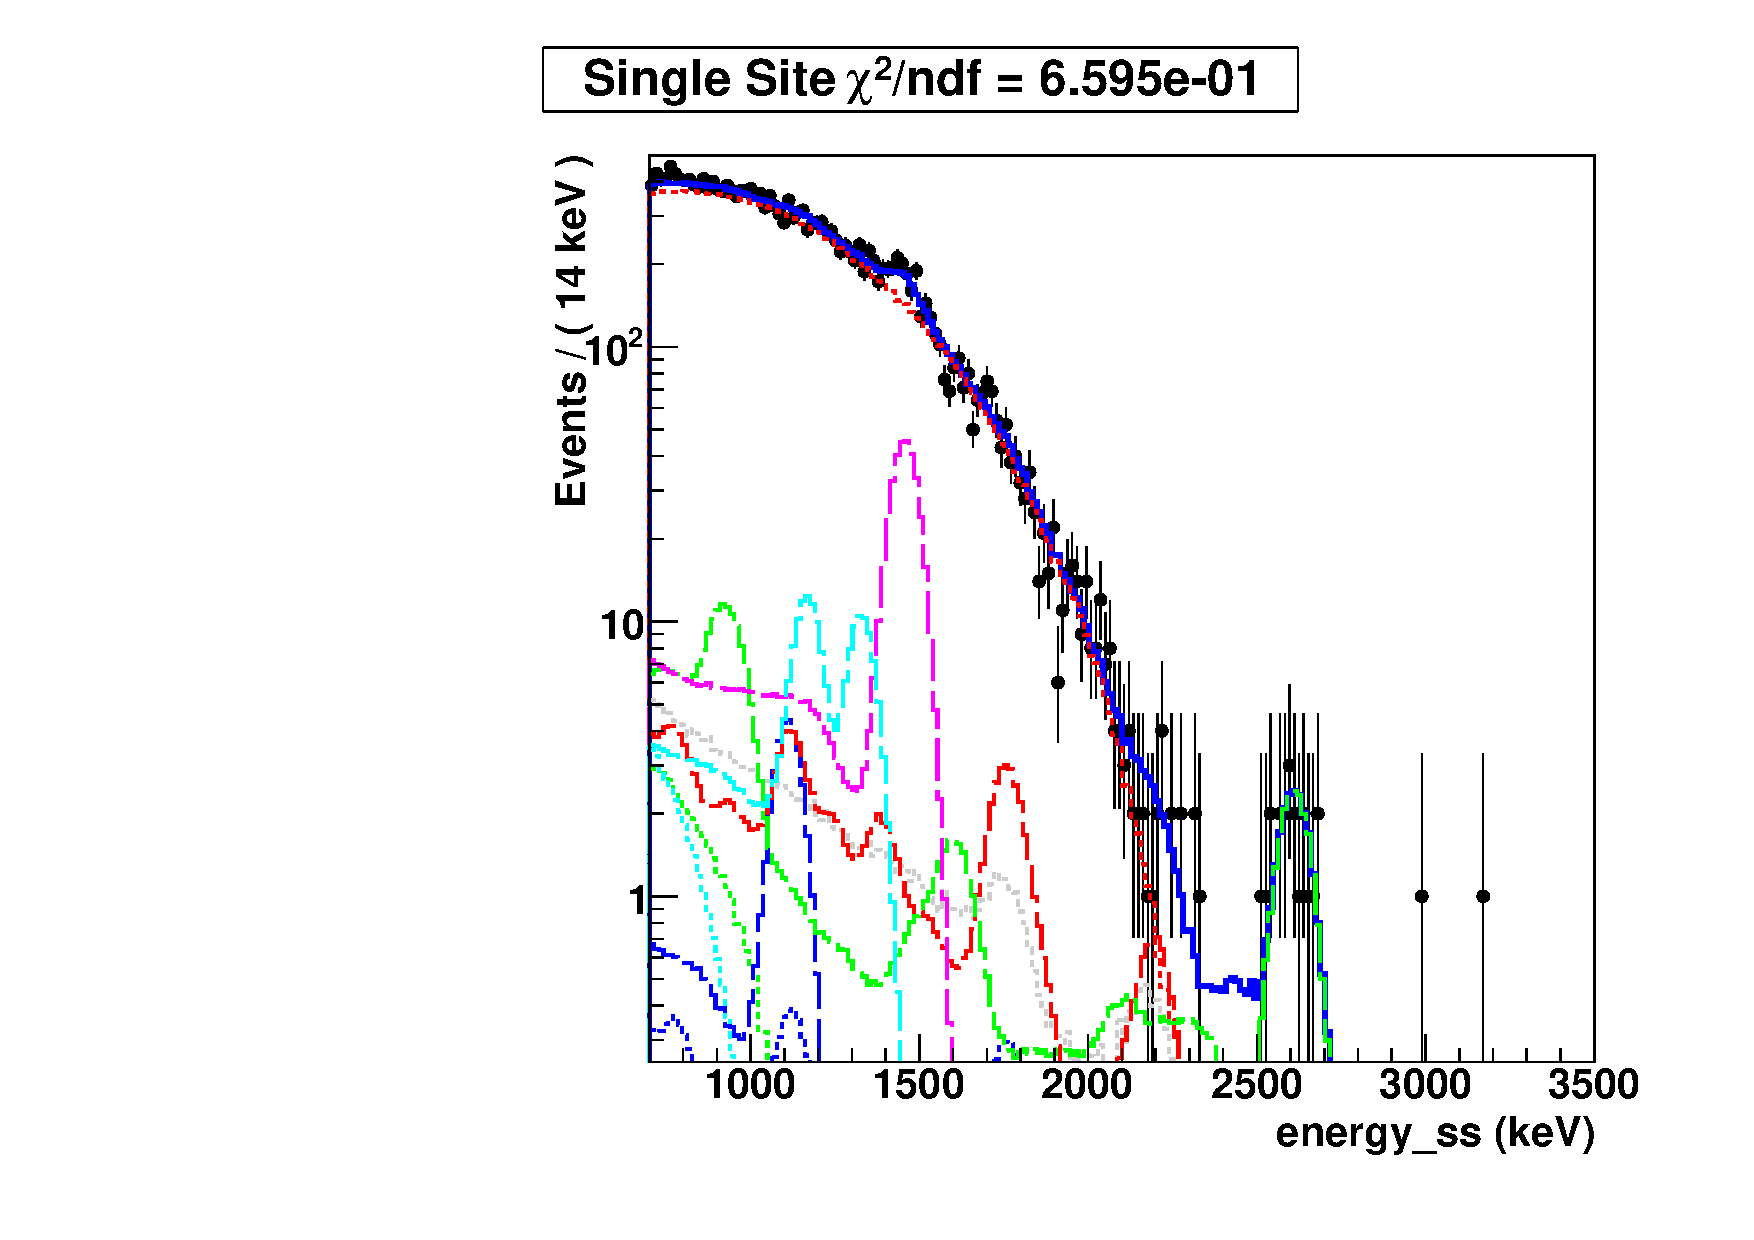
\includegraphics[width=\textwidth]{./plots/analysis_bb2n_best_fit_e_ss.pdf}
	\end{subfigure}\hfill%
	\begin{subfigure}[c]{0.48\textwidth}
	\centering
	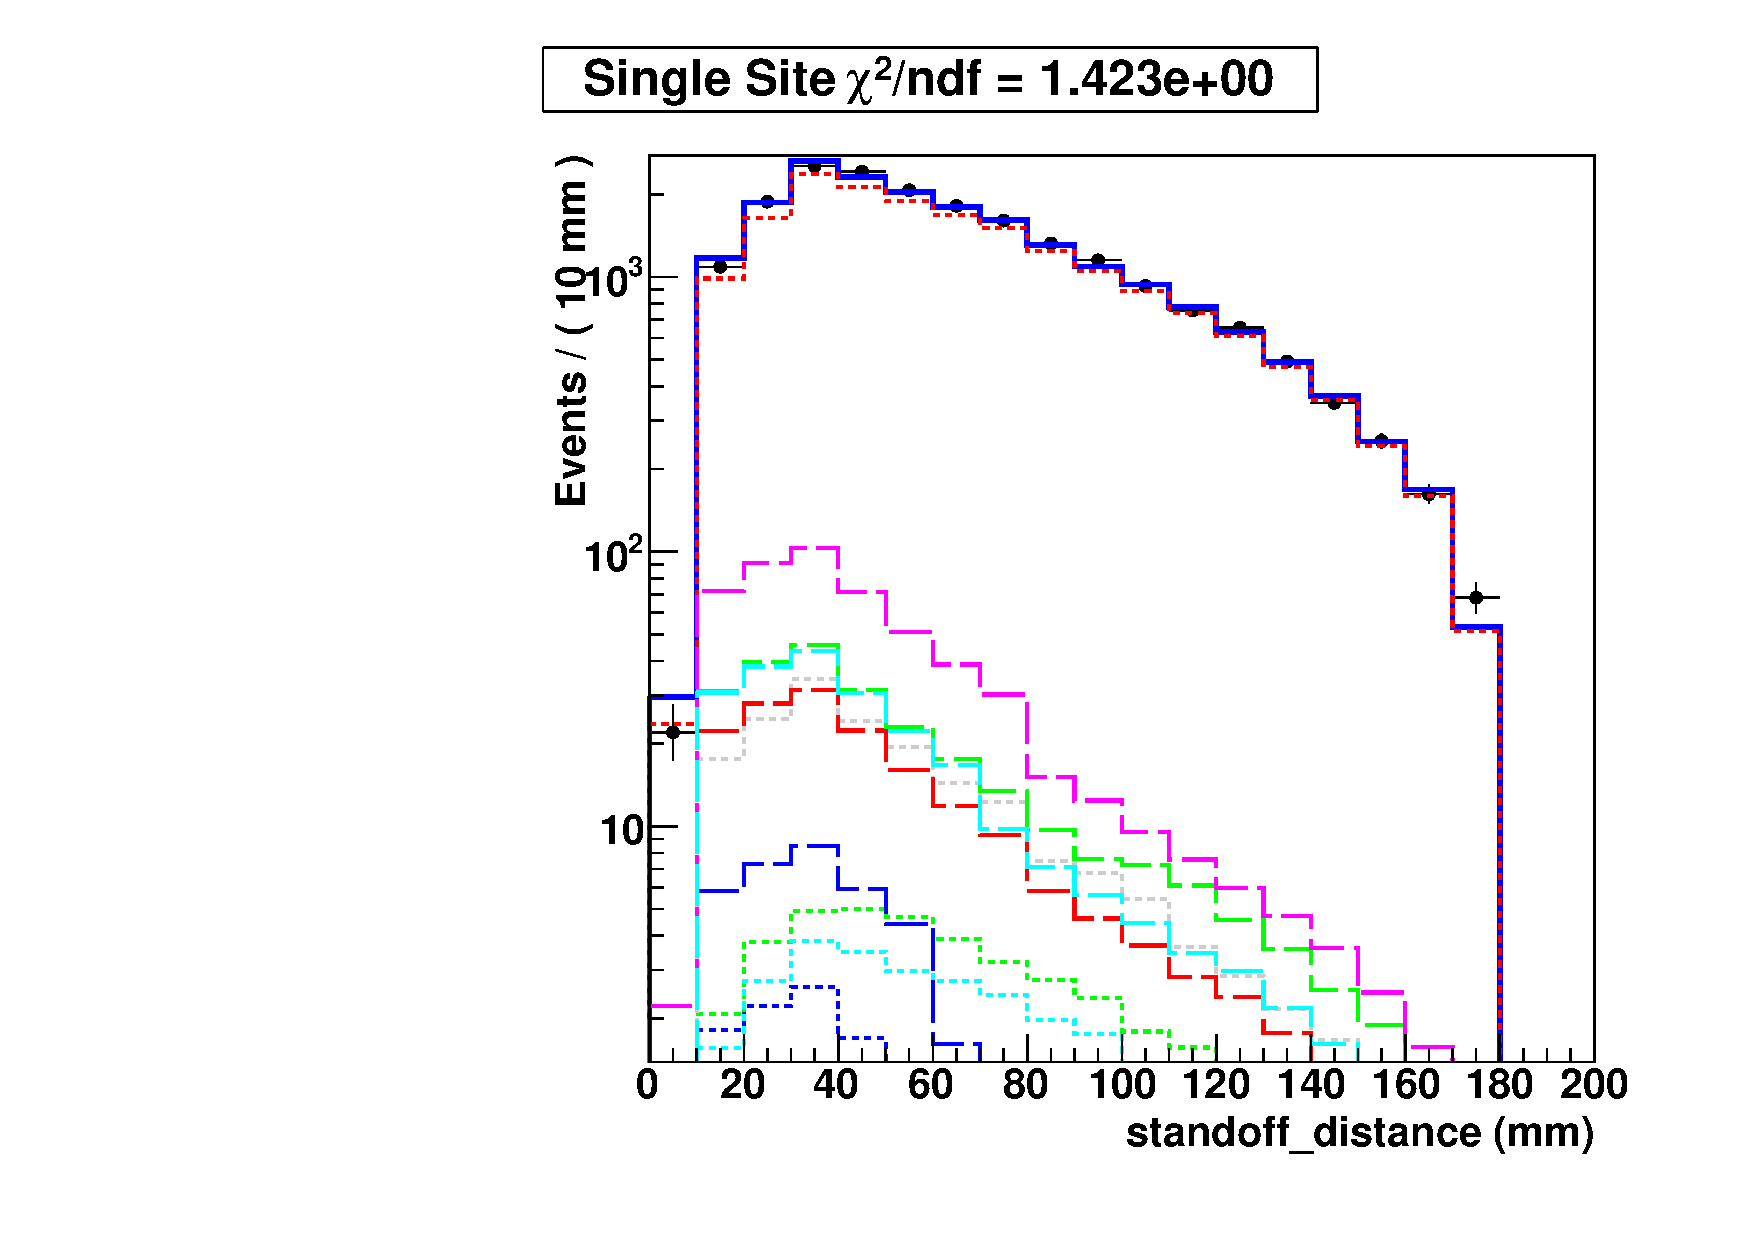
\includegraphics[width=\textwidth]{./plots/analysis_bb2n_best_fit_s_ss.pdf}
	\end{subfigure}
	\begin{subfigure}[c]{0.48\textwidth}
	\centering
	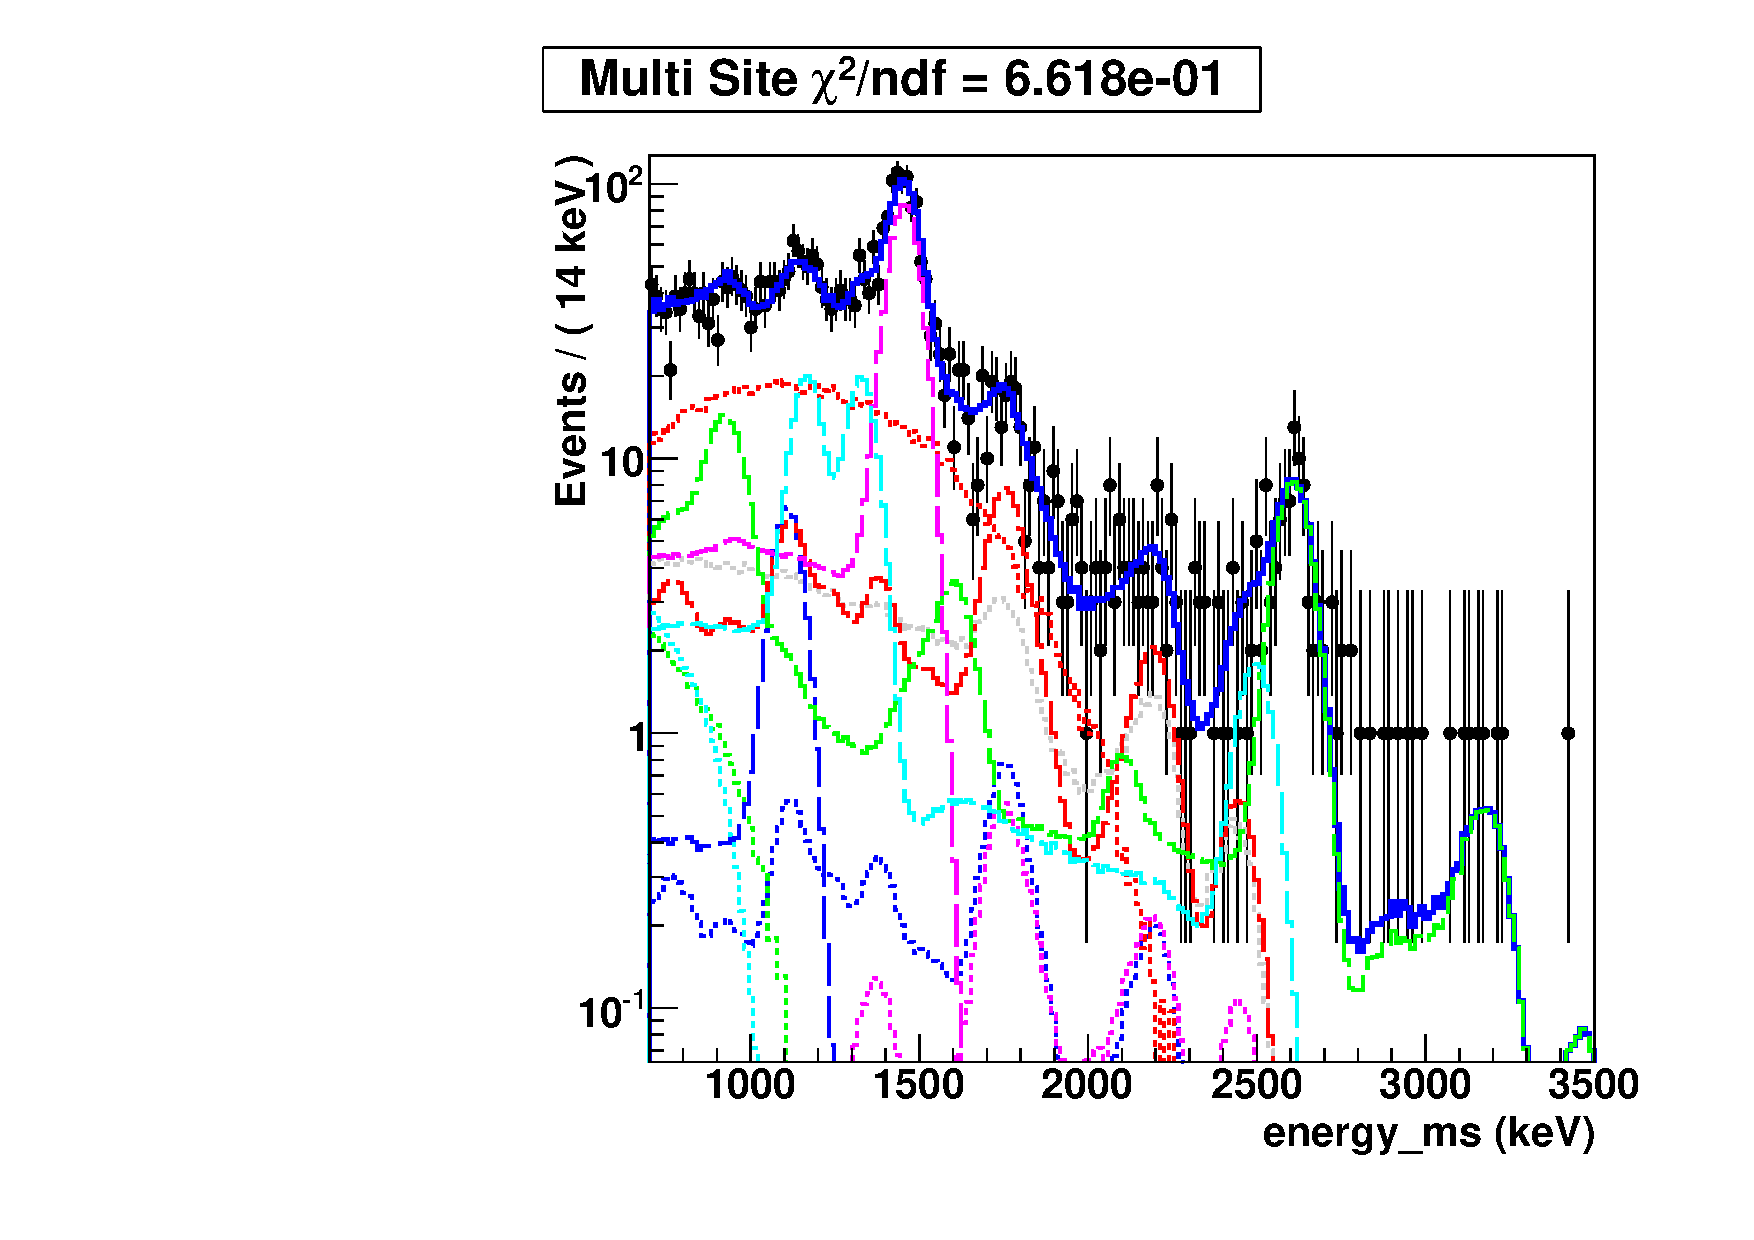
\includegraphics[width=\textwidth]{./plots/analysis_bb2n_best_fit_e_ms.pdf}
	\end{subfigure}\hfill%
	\begin{subfigure}[c]{0.48\textwidth}
	\centering
	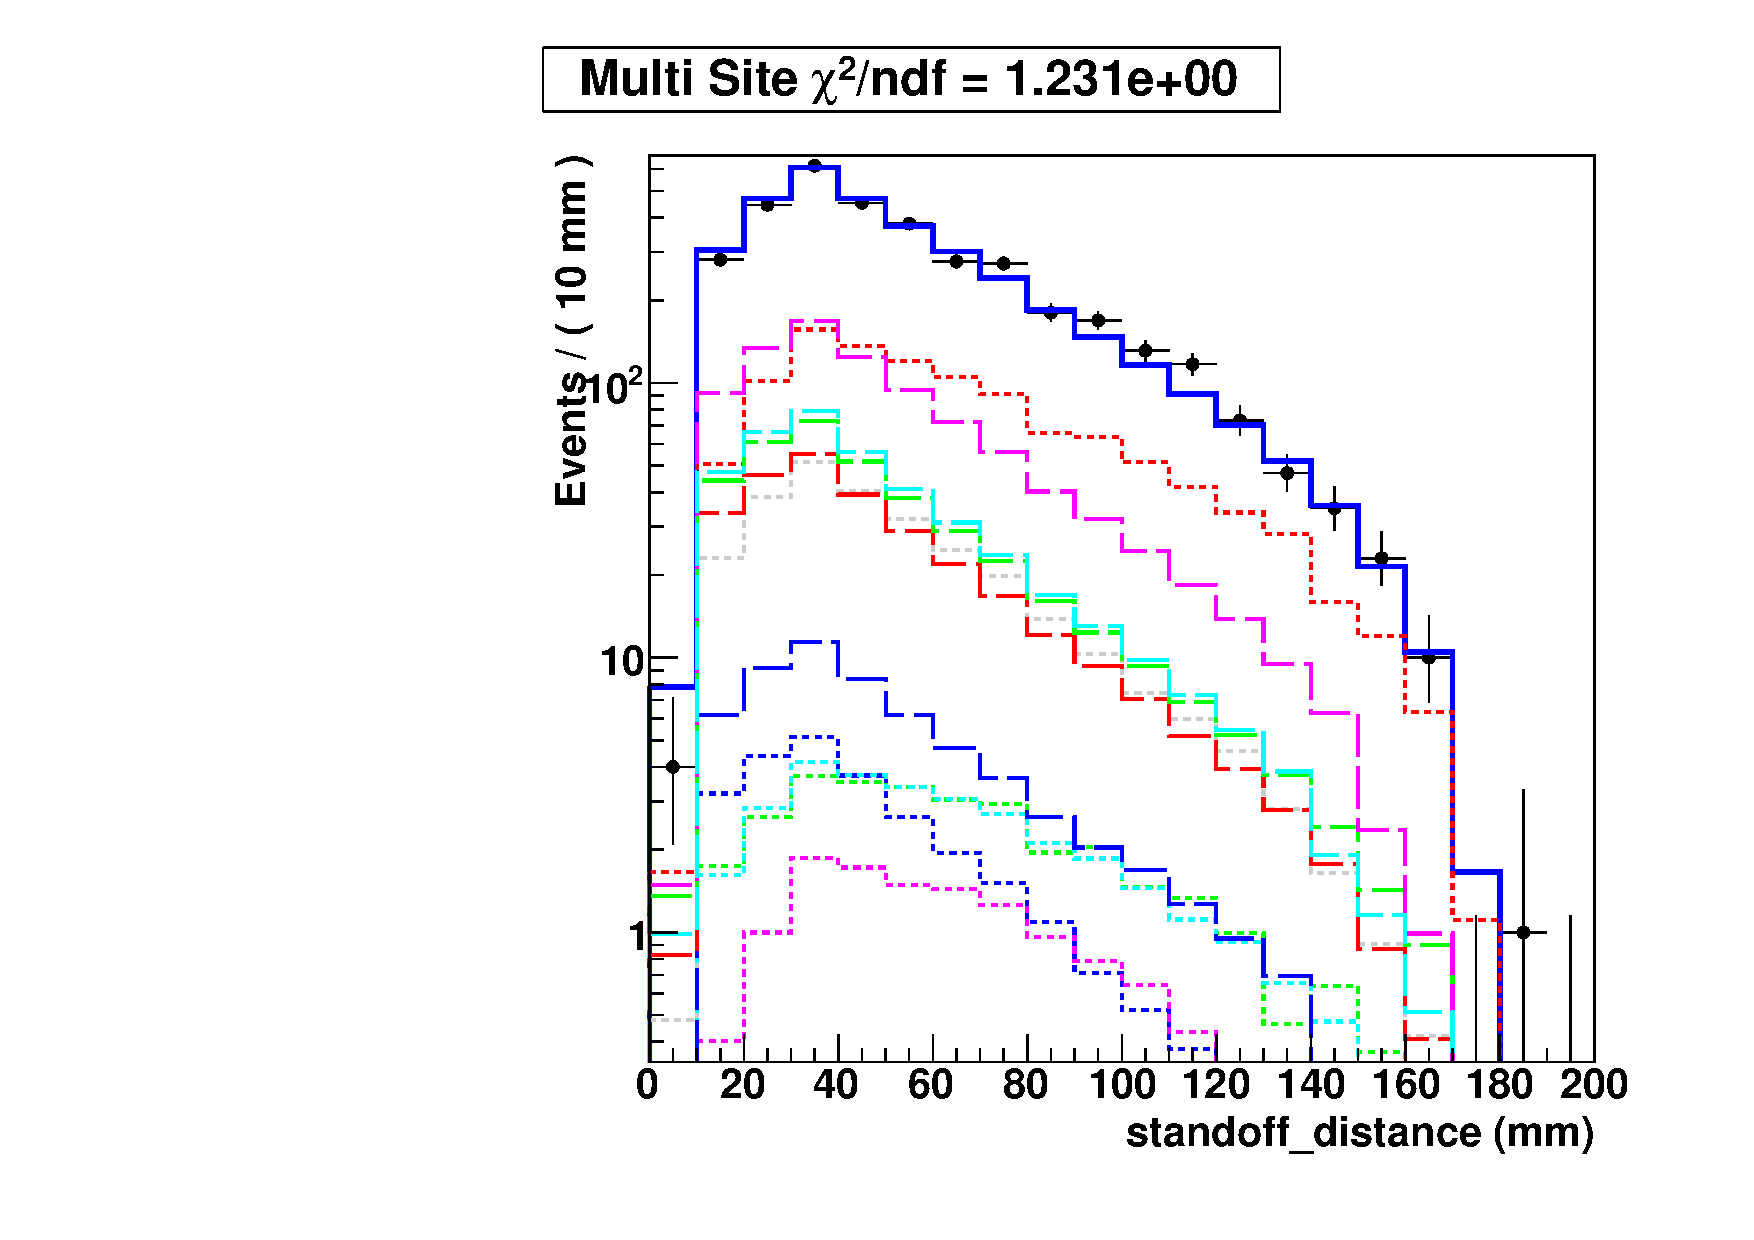
\includegraphics[width=\textwidth]{./plots/analysis_bb2n_best_fit_s_ms.pdf}
	\end{subfigure}
	\begin{subfigure}[c]{\textwidth}
	\centering
	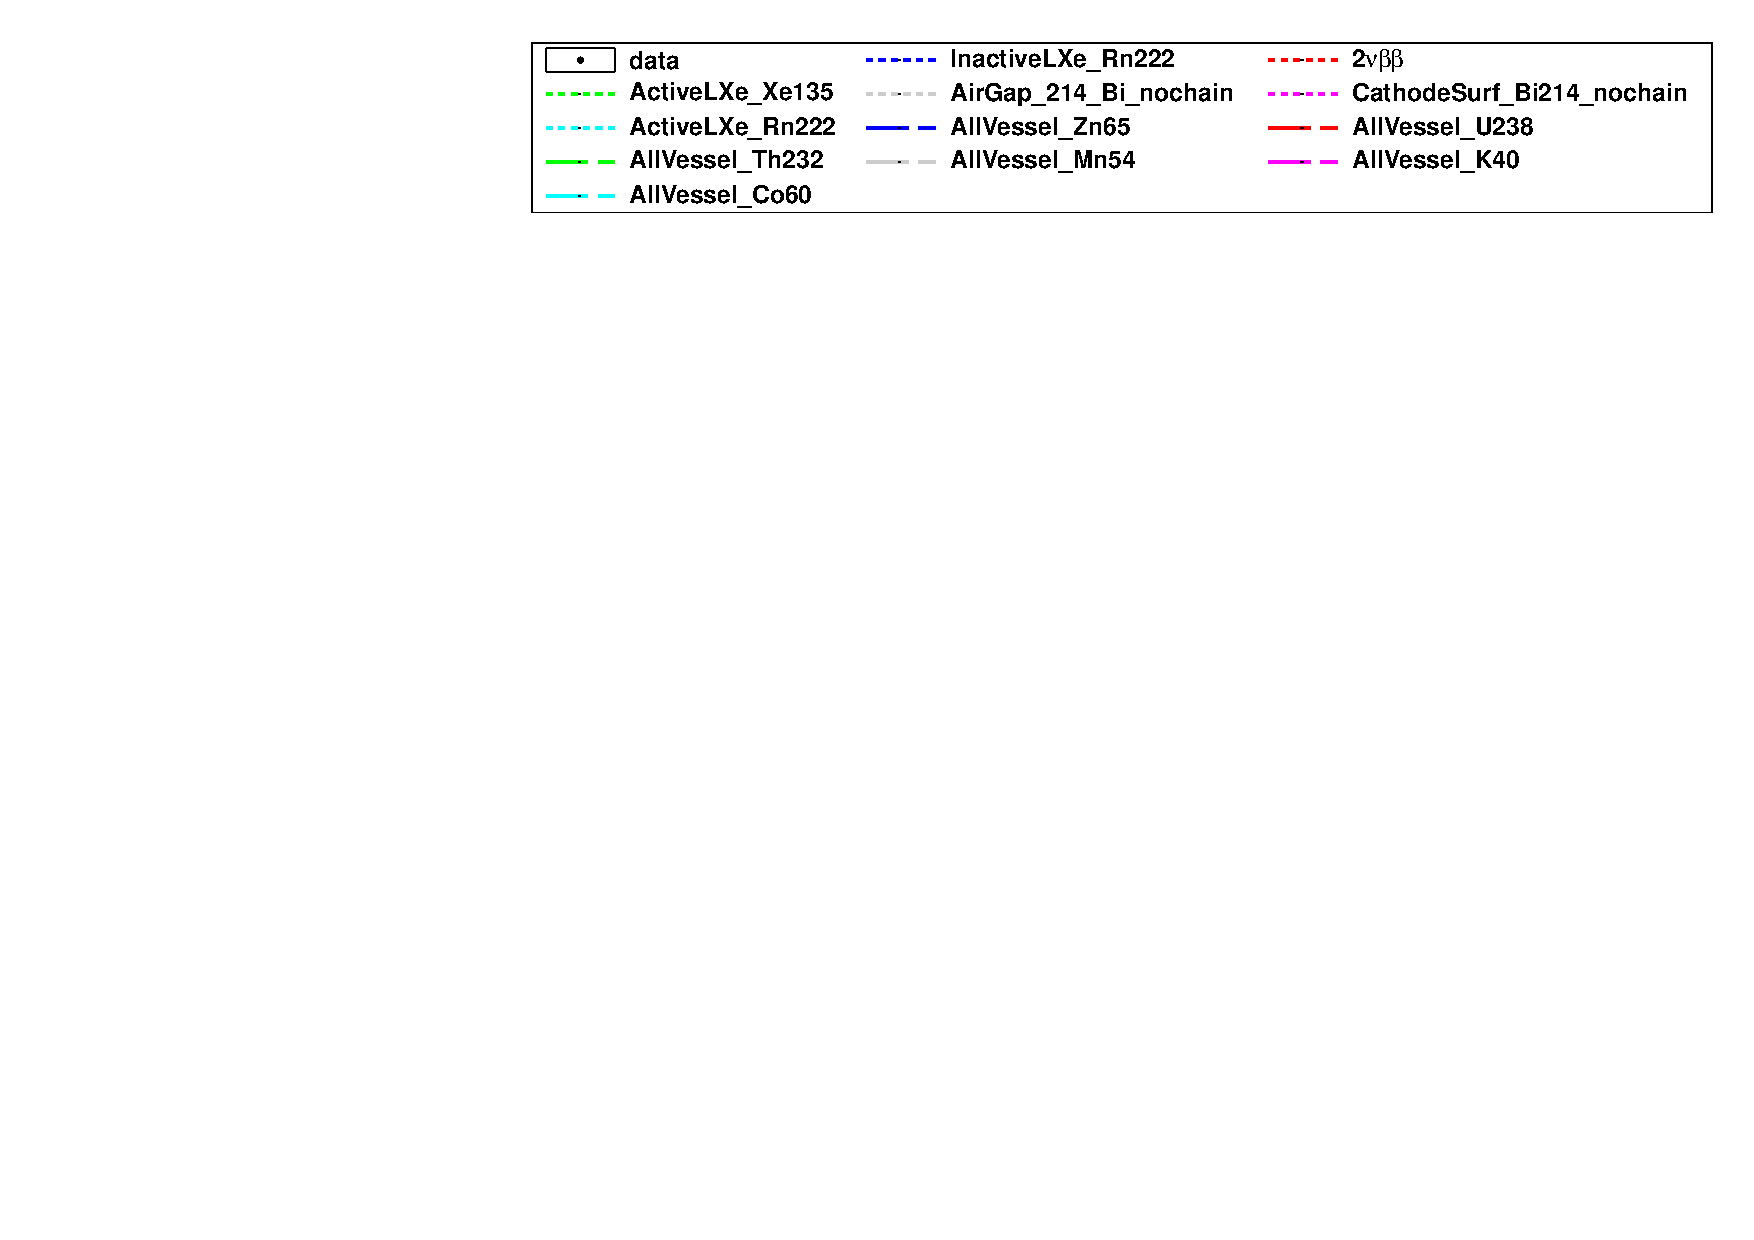
\includegraphics[width=\textwidth]{./plots/analysis_bb2n_best_fit_legend.pdf}
	\end{subfigure}
\caption[The best fit for \twonu{} to the data]{The best fit of \twonu{} and all background components to the data. The legend is shown at bottom. A projection of the energy spectrum is shown on the left, and a projection of the standoff distance spectrum is shown right. Single site events are shown at the top, while multiple site events are shown below.}
\label{fig:analysis_bb2n_best_fit}
\end{figure}

The best fit of the background and signal PDFs to the data is shown in \cref{fig:analysis_bb2n_best_fit}. The fiducial volume contains \SI{81.9}{\kg} of xenon, of which \SI{80.6}{\percent} is \isotope{136}{Xe}. The total live time was \SI{116.5}{day} and the efficiency for detecting \twonu{} after all cuts is \SI{60}{\percent}. The best fit using the maximum likelihood method says the data set contains \num{1.91e4} \twonu{} decays. This implies a half life of \SI{2.04e21}{\year}. \Cref{fig:analysis_bb2n_best_fit} shows projections of the best fit spectra.

\subsection{Effects of systematic errors}
Ultimately, the profile likelihood method gives an overall error, not broken down into statistical and systematic components. However, the relative contributions to the overall error can be obtained by fixing various components in the fit and observing the change in the width of the likelihood profile. The statistical uncertainty is obtained by fixing all parameters except the number of \twonu{} events to their best fit values. Systematic uncertainty can likewise be obtained by looking at just the effect of the single site fraction uncertainty, the contributions of the background PDFs, and the normalization uncertainty. \Cref{tab:analysis_error_budget} breaks down these different sources of uncertainty.

\begin{table}[htbp]
\centering
\caption[Effect of uncertainties on the half life measurement]{A breakdown of the various uncertainties on the measurement of the \twonu{} half life. Each contribution is given as a percentage of the best-fit value obtained by letting only the specified parameter float when performing a profile scan of the likelihood function. Correlations mean they do not sum in quadrature.}
\label{tab:analysis_error_budget}
\begin{tabular}{c c}\toprule
Uncertainty	&	Contribution (\%)	\\\midrule
Statistical		&	0.76				\\
SS fraction	&	0.78				\\
Backgrounds	&	0.83				\\
Normalization	&	2.35				\\\midrule
\textbf{Total}	&	\textbf{3.76}		\\\bottomrule
\end{tabular}
\end{table}

Thus, the measurement of the \twonu{} half life for \isotope{136}{Xe} is
\begin{equation}
T_{1/2} = \left ( 2.04 \pm 0.015 (\text{stat}) \pm 0.075 (\text{sys}) \right)\times 10^{21} \si{\year}
\label{eq:analysis_bb2n_halflife}
\end{equation}

\subsection{Consistency Checks}
\subsubsection{Time and Position Independence}
As \cref{fig:analysis_bb2n_rate_v_time} shows, the half life obtained by fitting over subsets of the data is consistent with the half life obtained from the entire data set. Thus, the half life seems steady over time. Likewise, as \cref{fig:analysis_bb2n_rate_v_pos} shows, the \twonu{} decays seem uniformly distributed throughout the volume.

\begin{figure}[htbp]
\centering
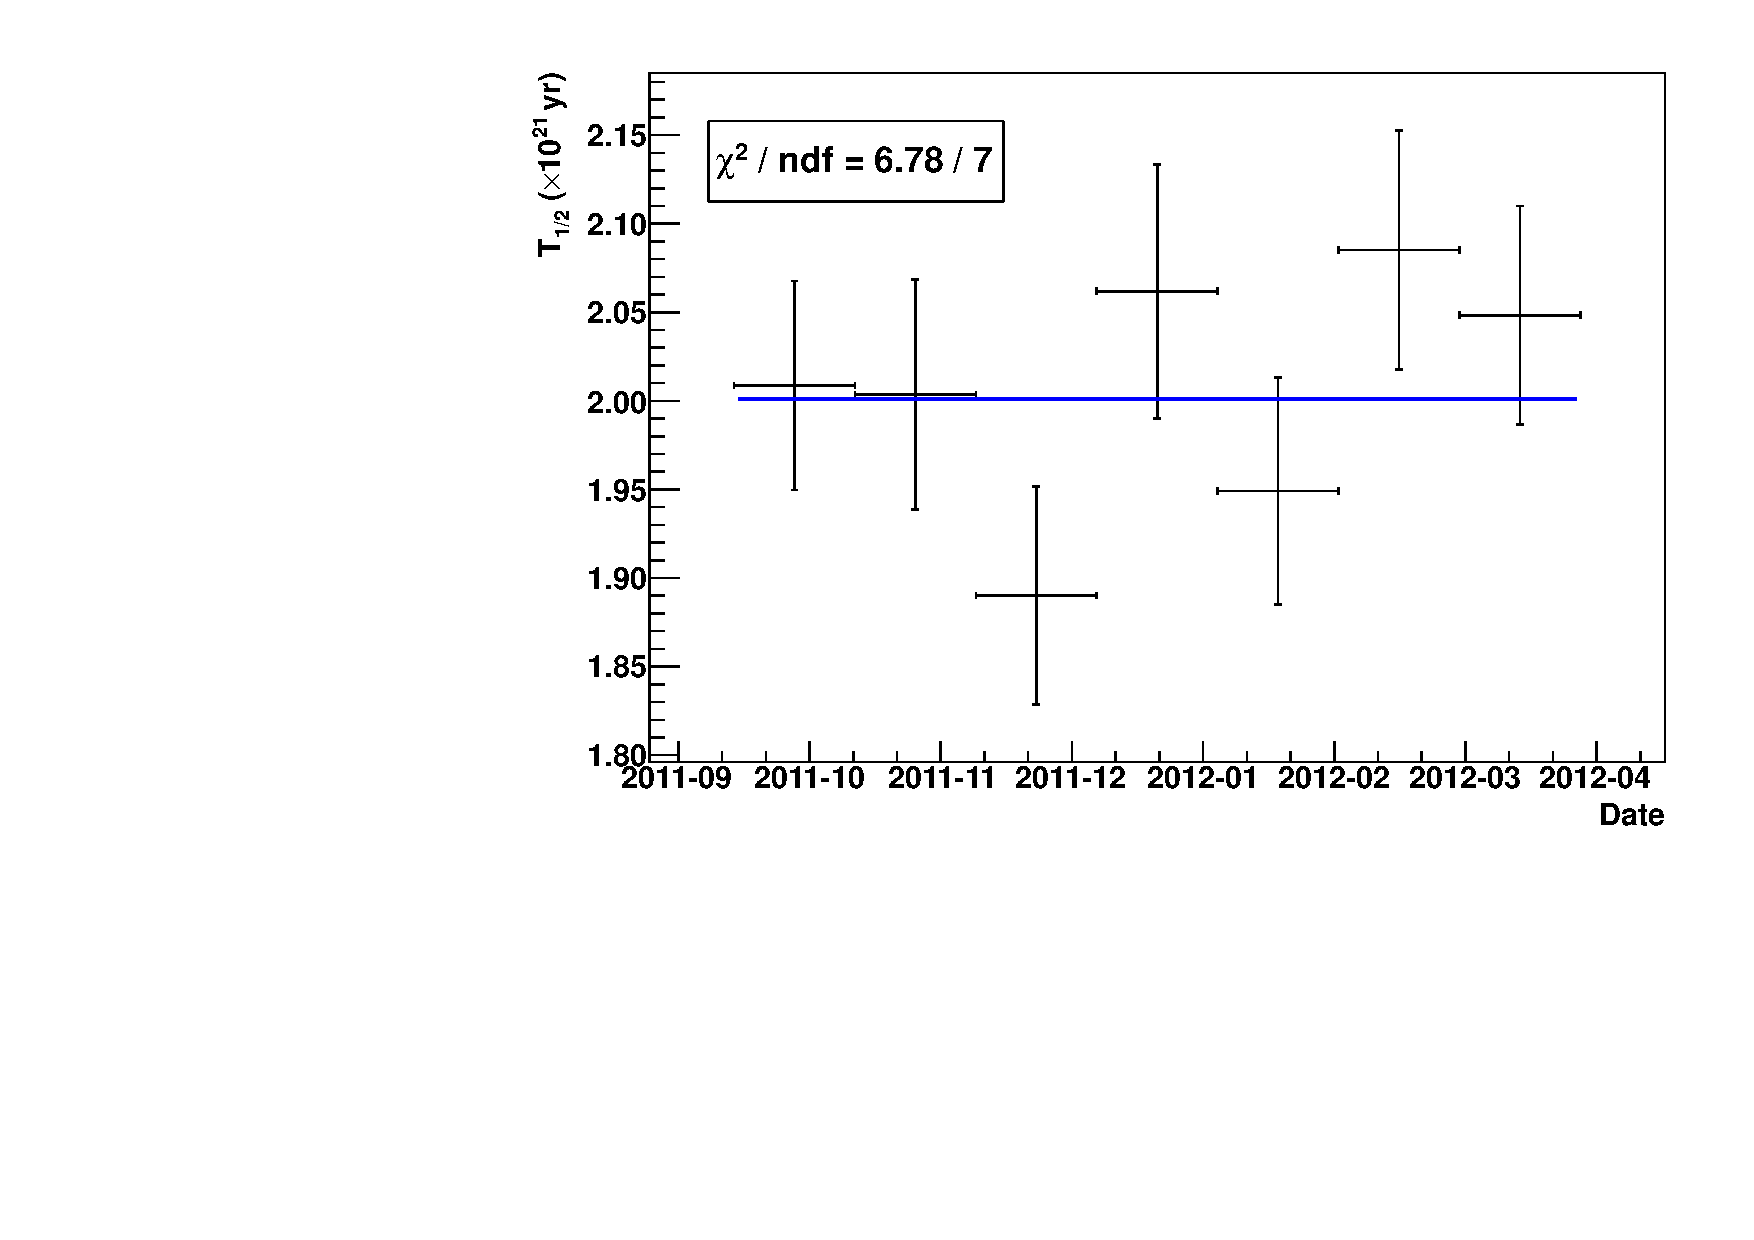
\includegraphics[width=0.6\textwidth]{./plots/analysis_bb2n_rate_v_time.pdf}
\caption[\twonu{} half life vs. time]{The half life of \twonu{} throughout the data set. The data set has been broken up into 4 week slices and each individual period has been fit in order to determine the half life. The error bars do not include the normalization uncertainty, which is a systematic error shared by all fits. The blue line represents the best fit half life for the entire data set, as reported in \cref{eq:analysis_bb2n_halflife}. The \(\chi^2\) statistic comparing this value to the individual time periods shows good agreement.}
\label{fig:analysis_bb2n_rate_v_time}
\end{figure}

\begin{figure}[htbp]
	\begin{subfigure}[c]{0.48\textwidth}
	\centering
	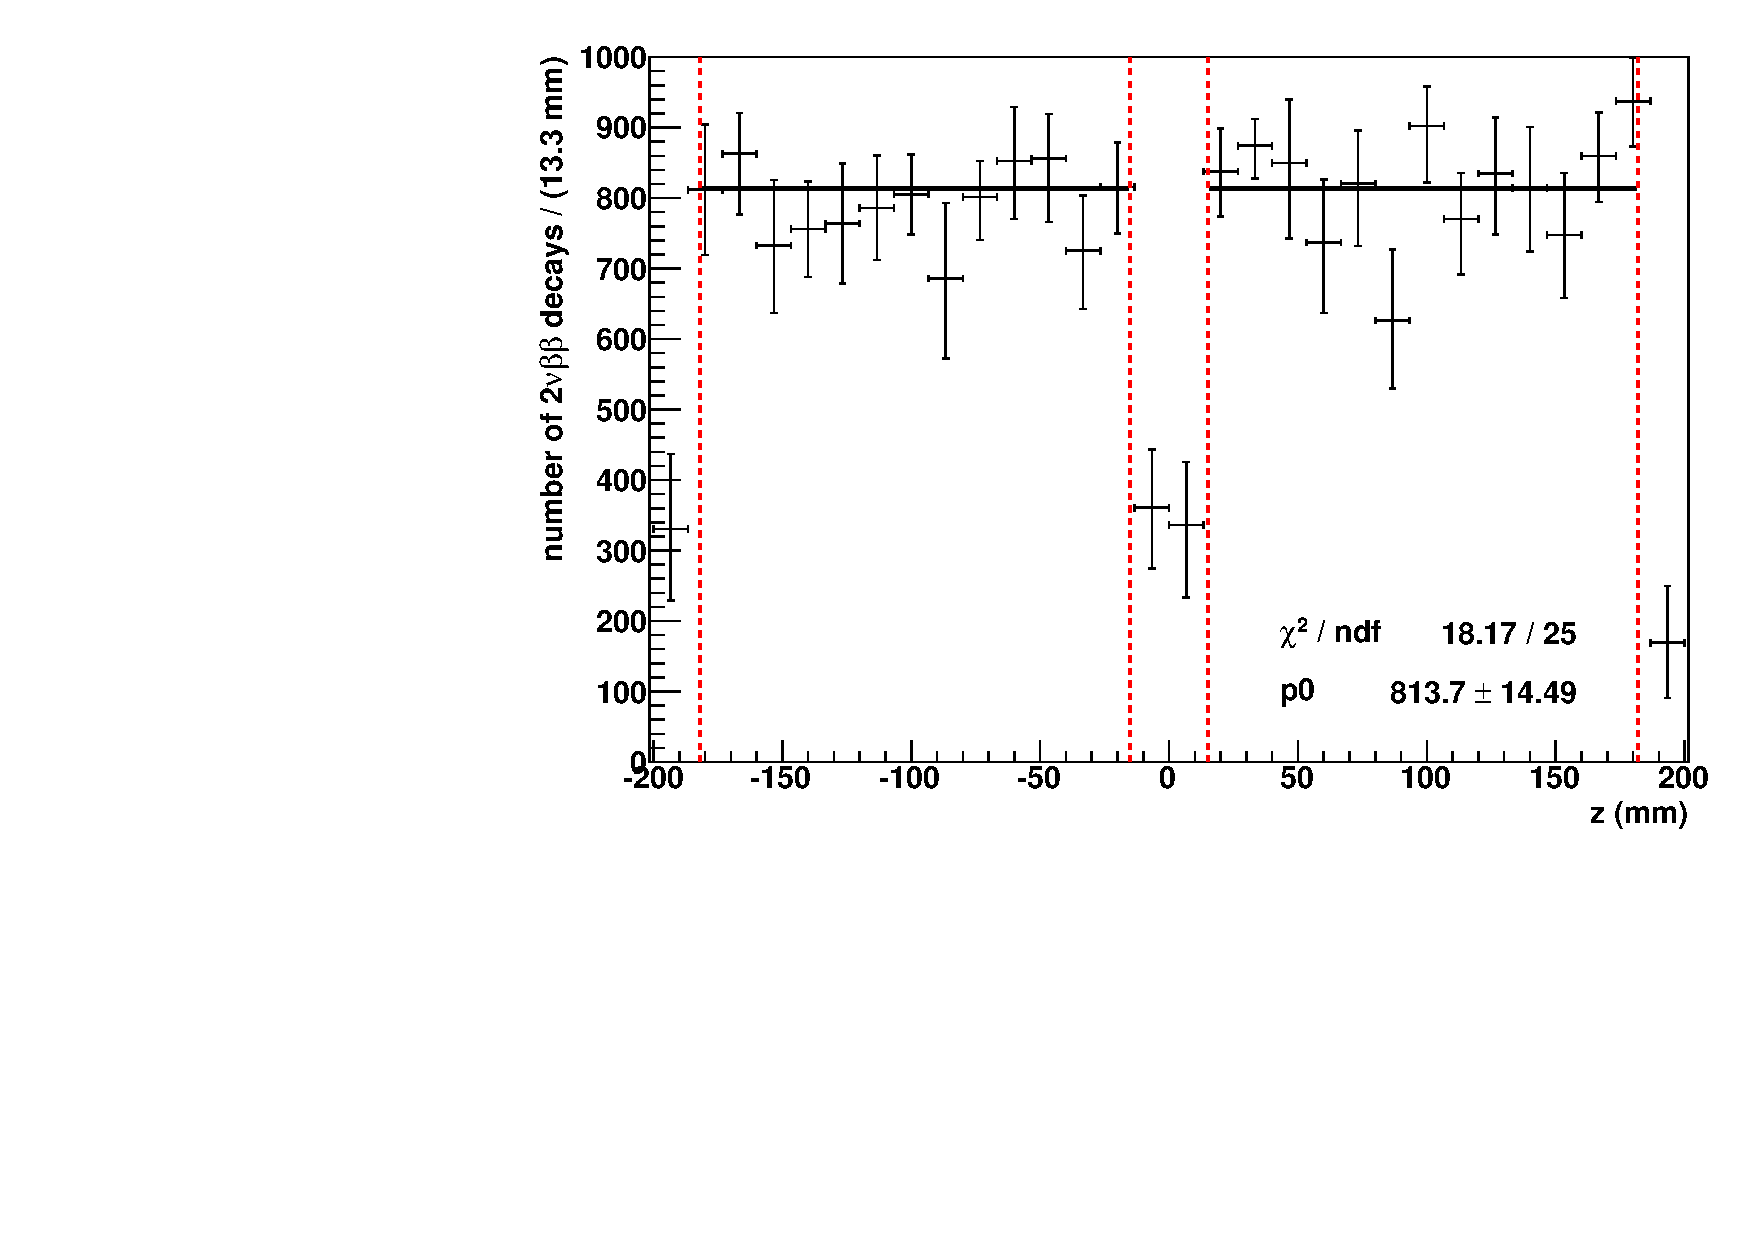
\includegraphics[width=\textwidth]{./plots/analysis_bb2n_rate_v_z.pdf}
	\end{subfigure}\hfill%
	\begin{subfigure}[c]{0.48\textwidth}
	\centering
	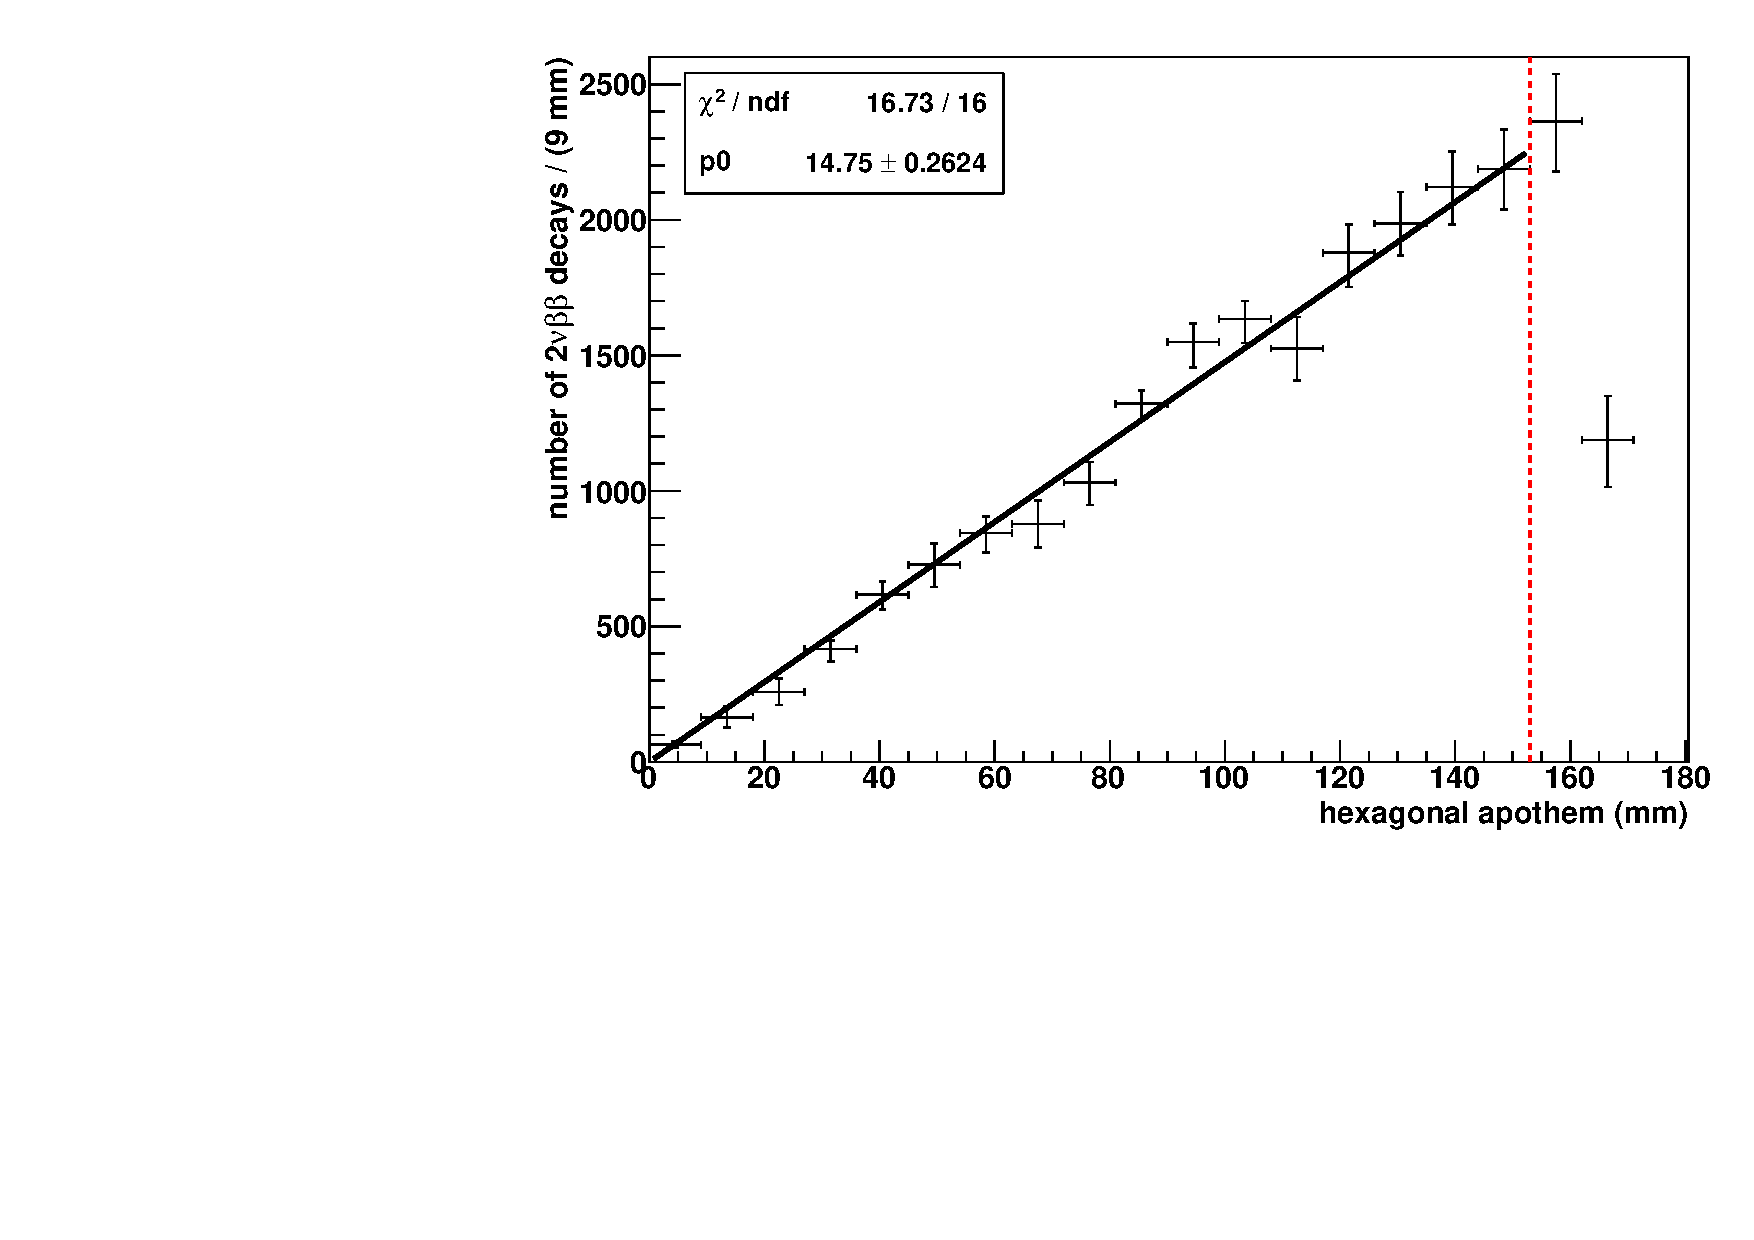
\includegraphics[width=\textwidth]{./plots/analysis_bb2n_rate_v_apothem.pdf}
	\end{subfigure}
\caption[Number of \twonu{} decays vs. position]{The number of \twonu{} decays returned by the fit when applied to small volumes of the detector. As the plot on the left shows, the rate is consistent with uniformity in \(z\). For the right plot, the volume is proportional to the square of the apothem. Therefore, the volume in a shell bounded by apothem \(r\) and \(r+dr\) should increase linearly as a function of \(r\). Thus, the plot shows the \twonu{} decays are uniformly distributed throughout the fiducial volume.}
\label{fig:analysis_bb2n_rate_v_pos}
\end{figure}

\subsubsection{Energy-Only Fit}
It is worthwhile to verify that the inclusion of standoff distance in the fit is not somehow biasing the results. Repeating the fit with the standoff distance ignored, the best fit for the \twonu{} half life is \(T_{1/2} = \SI{2.06\pm0.08e21}{\year}\), in agreement with the half life reported above.

\subsection{Comparison to Previous Results}
\Cref{fig:analysis_bb2n_half_life_comparison} shows previous measurements of the \twonu{} half life by the EXO-200 and KamLAND-Zen experiments. The Run2a data was previously used to report \(T_{1/2} = (2.23\pm0.017(\text{stat})\pm0.22(\text{sys}))\times10^{21}\si{\year}\). This measurement suffered from a 3\% overestimate in the detector live time, and correcting for this brings the measurement closer to the one reported here. That measurement also used a larger fiducial volume, including regions near the detector edges where the volume is less well-known (this is demonstrated by the apparent drop-off in events near the walls and anode/cathode planes in \cref{fig:analysis_bb2n_rate_v_pos}). So while this measurement is consistent with previous measurements by the EXO-200 experiment, it is now in tension with the measurements by KamLAND-Zen.

\begin{figure}[htbp]
\centering
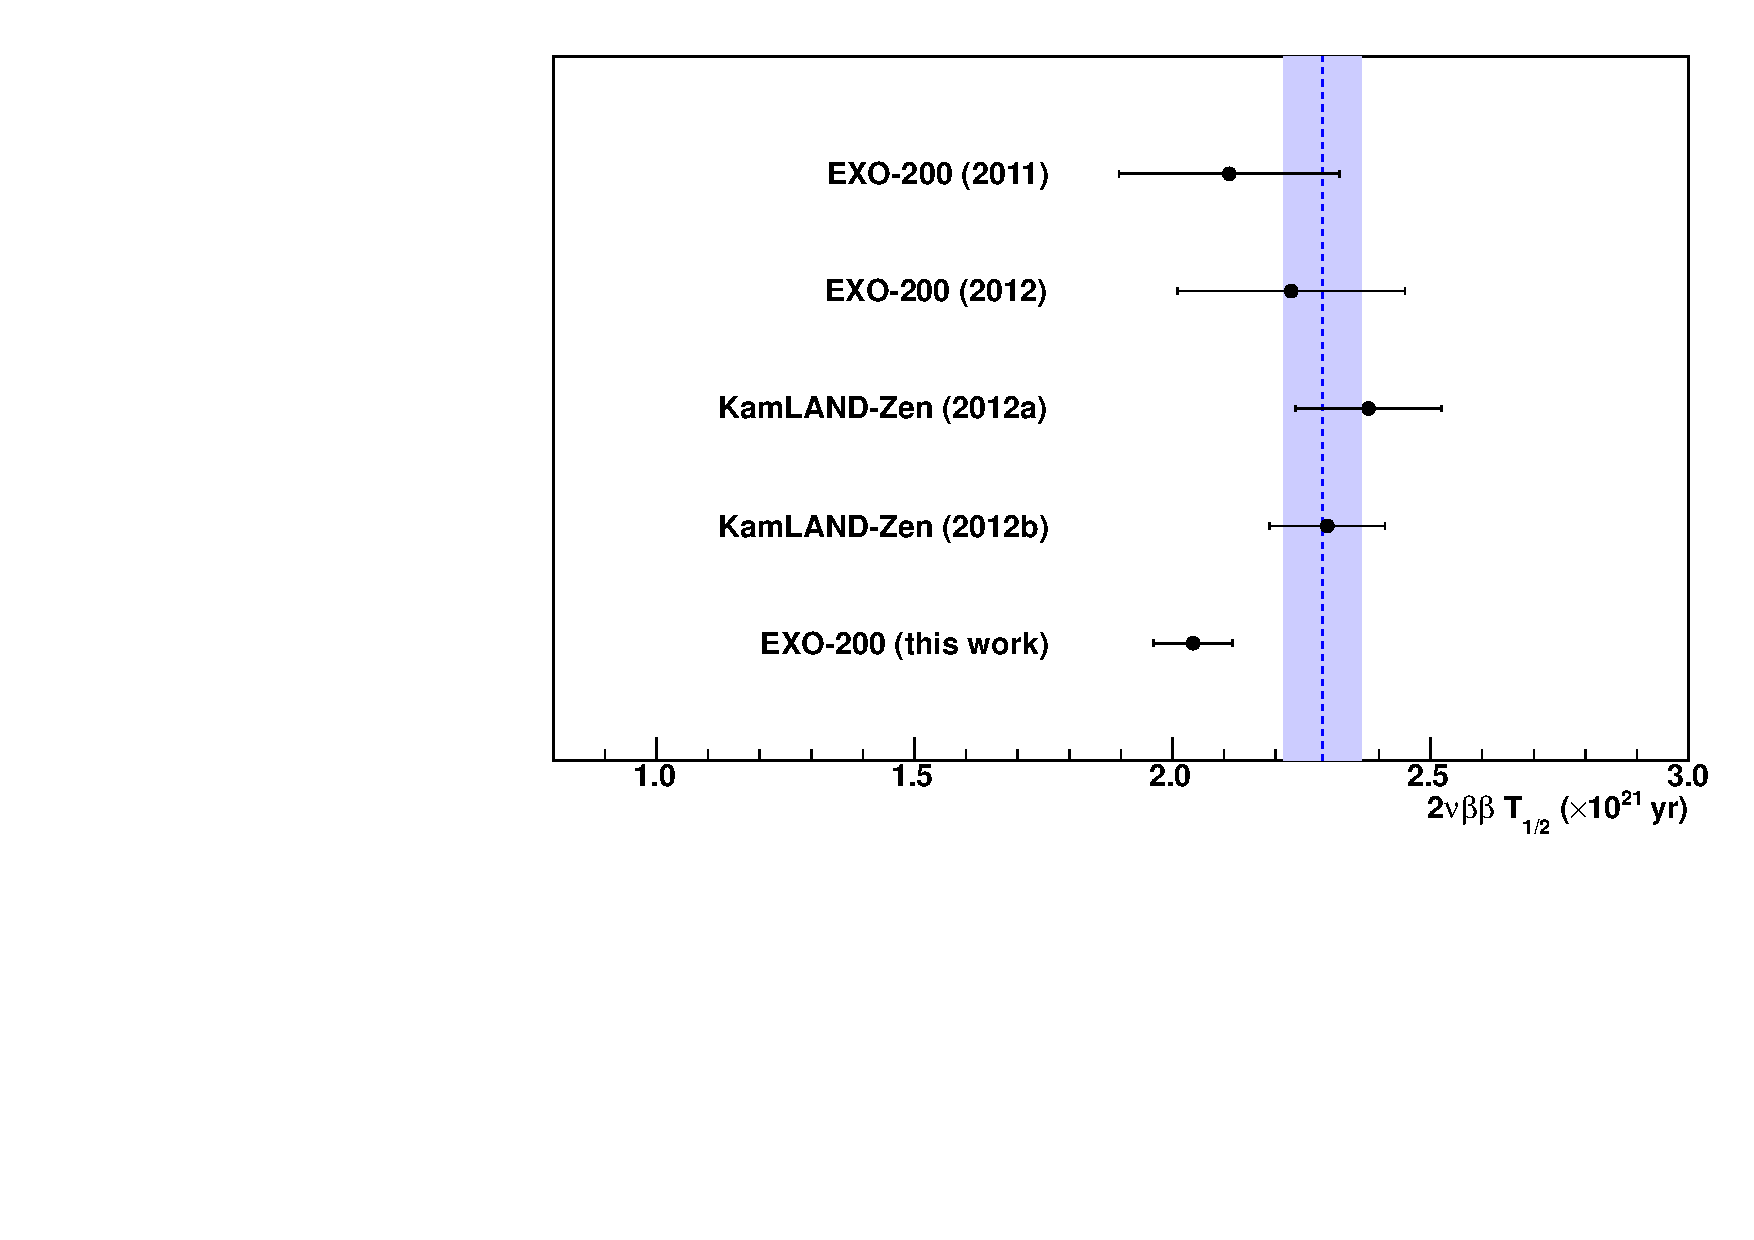
\includegraphics[width=0.6\textwidth]{./plots/analysis_bb2n_half_life_comparison.pdf}
\caption[Comparison of measurements of the half life for \twonu{}]{A comparison of measurements of \twonu{} half life measurements. The EXO-200 experiment reported results in 2011 \cite{Ackerman:2011gz} and 2012 \cite{Auger:2012ar} using independent data sets. The KamLAND-Zen experiment reported two results in 2012, denoted a \cite{Gando:2012qy} and b \cite{Gando:2012fk}, with some data in common between the two analyses. The blue line are blue shaded area are the maximum likelihood estimate and the 1\(\sigma\) error on the half life (\(T_{1/2} = (2.29\pm0.076)\times10^{21}\si{\year}\)) based on these previous measurements, assuming all are independent. The bottom point is the measurement reported in this work.}
\label{fig:analysis_bb2n_half_life_comparison}
\end{figure}

\section{Limits on \(0\nu\beta\beta\chi^0(\chi^0)\)}
\subsection{Limits}
The Majoron-emitting modes are each separately included in the fit, and confidence intervals are constructed for each using the bounded likelihood method described above. All modes fit to a value consistent with zero events at the 68\% confidence level. The likelihood profiles used to extract the 90\% confidence limits are shown in \cref{fig:analysis_bb0nX_profiles}. Limits on the number of events are translated into limits on half lives using the known live time and number of \xenon{136} nuclei in the fiducial volume. The efficiency for detection is 90.0\% for the mode with spectral index 1; 85.7\% for the mode with spectral index 2; 77.4\% for the mode with spectral index 3; and 45.0\% for the mode with spectral index 7. \Cref{fig:analysis_bb0nX_best_fit} shows projections of the single site spectra with the 90\% confidence limits for the Majoron-emitting modes. \Cref{tab:analysis_majoron_limits} summarizes the limits obtained in the context of a number of models.

\begin{figure}[htbp]
\centering
	\begin{subfigure}[c]{0.48\textwidth}
	\centering
	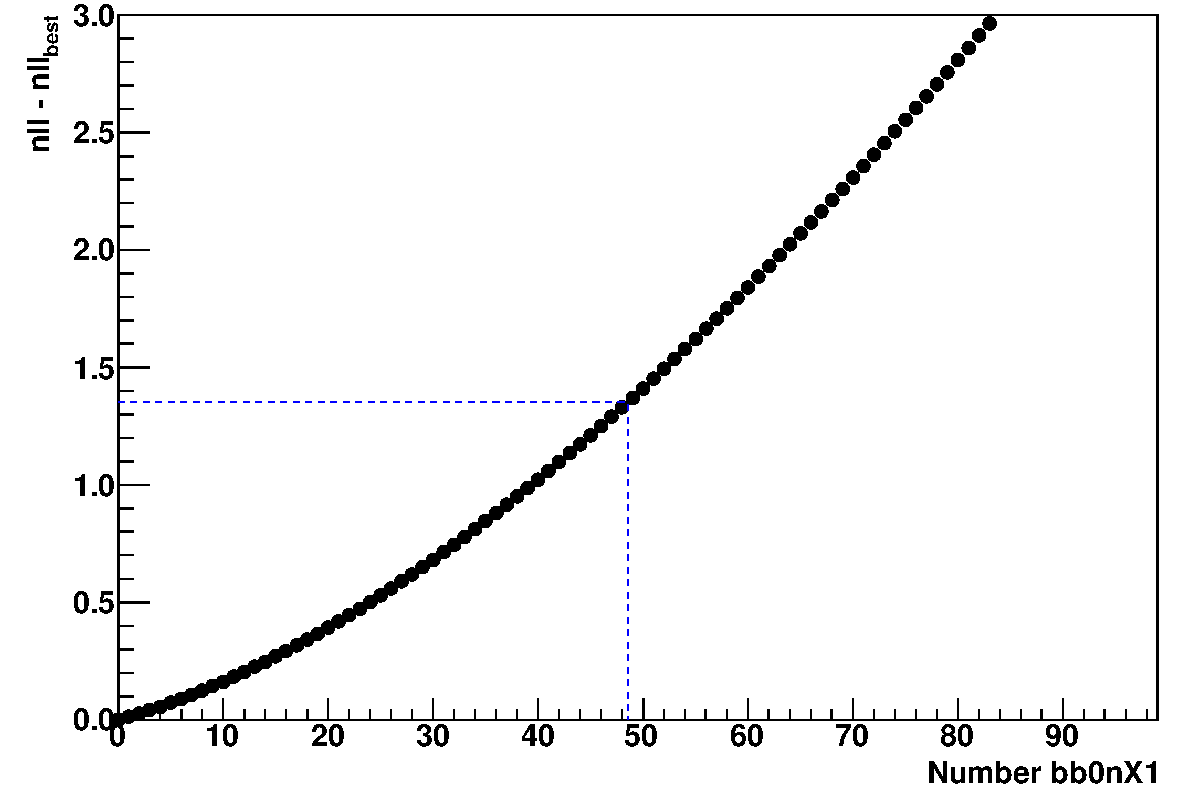
\includegraphics[width=\textwidth]{./plots/analysis_bb0nX1_profile.pdf}
	\end{subfigure}\hfill%
	\begin{subfigure}[c]{0.48\textwidth}
	\centering
	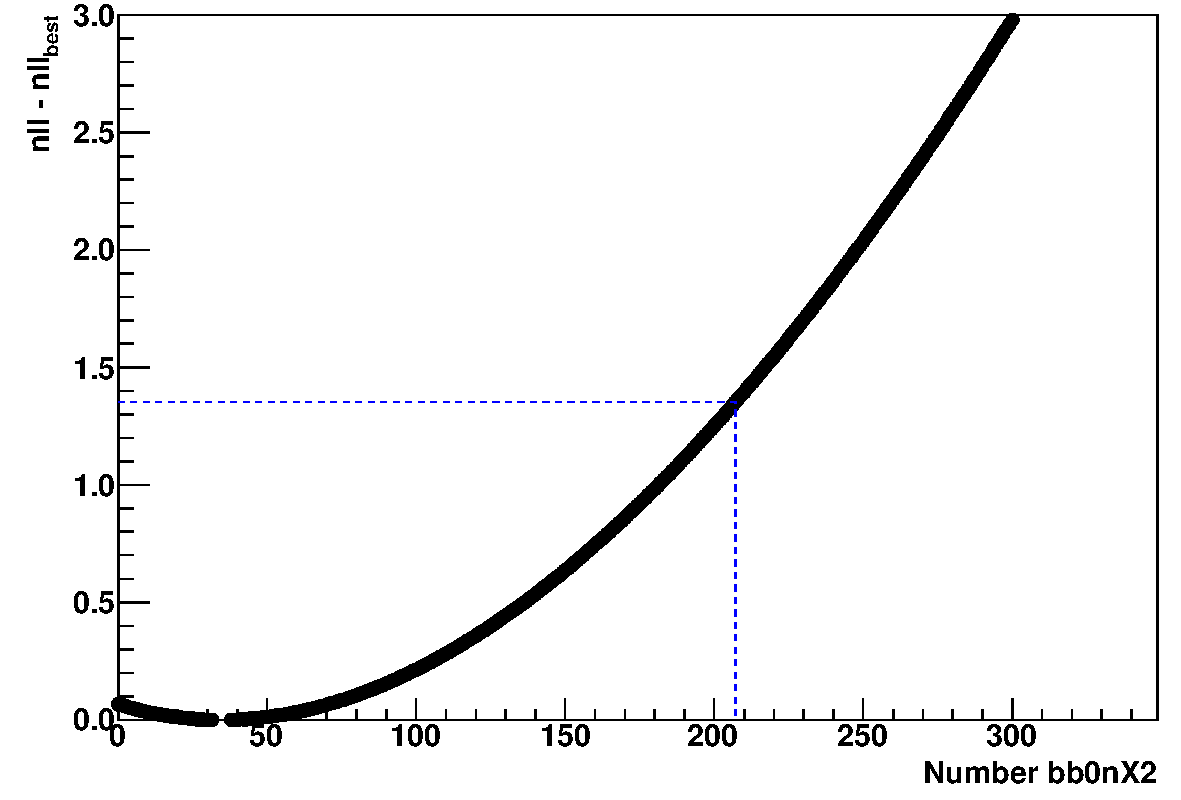
\includegraphics[width=\textwidth]{./plots/analysis_bb0nX2_profile.pdf}
	\end{subfigure}
	\begin{subfigure}[c]{0.48\textwidth}
	\centering
	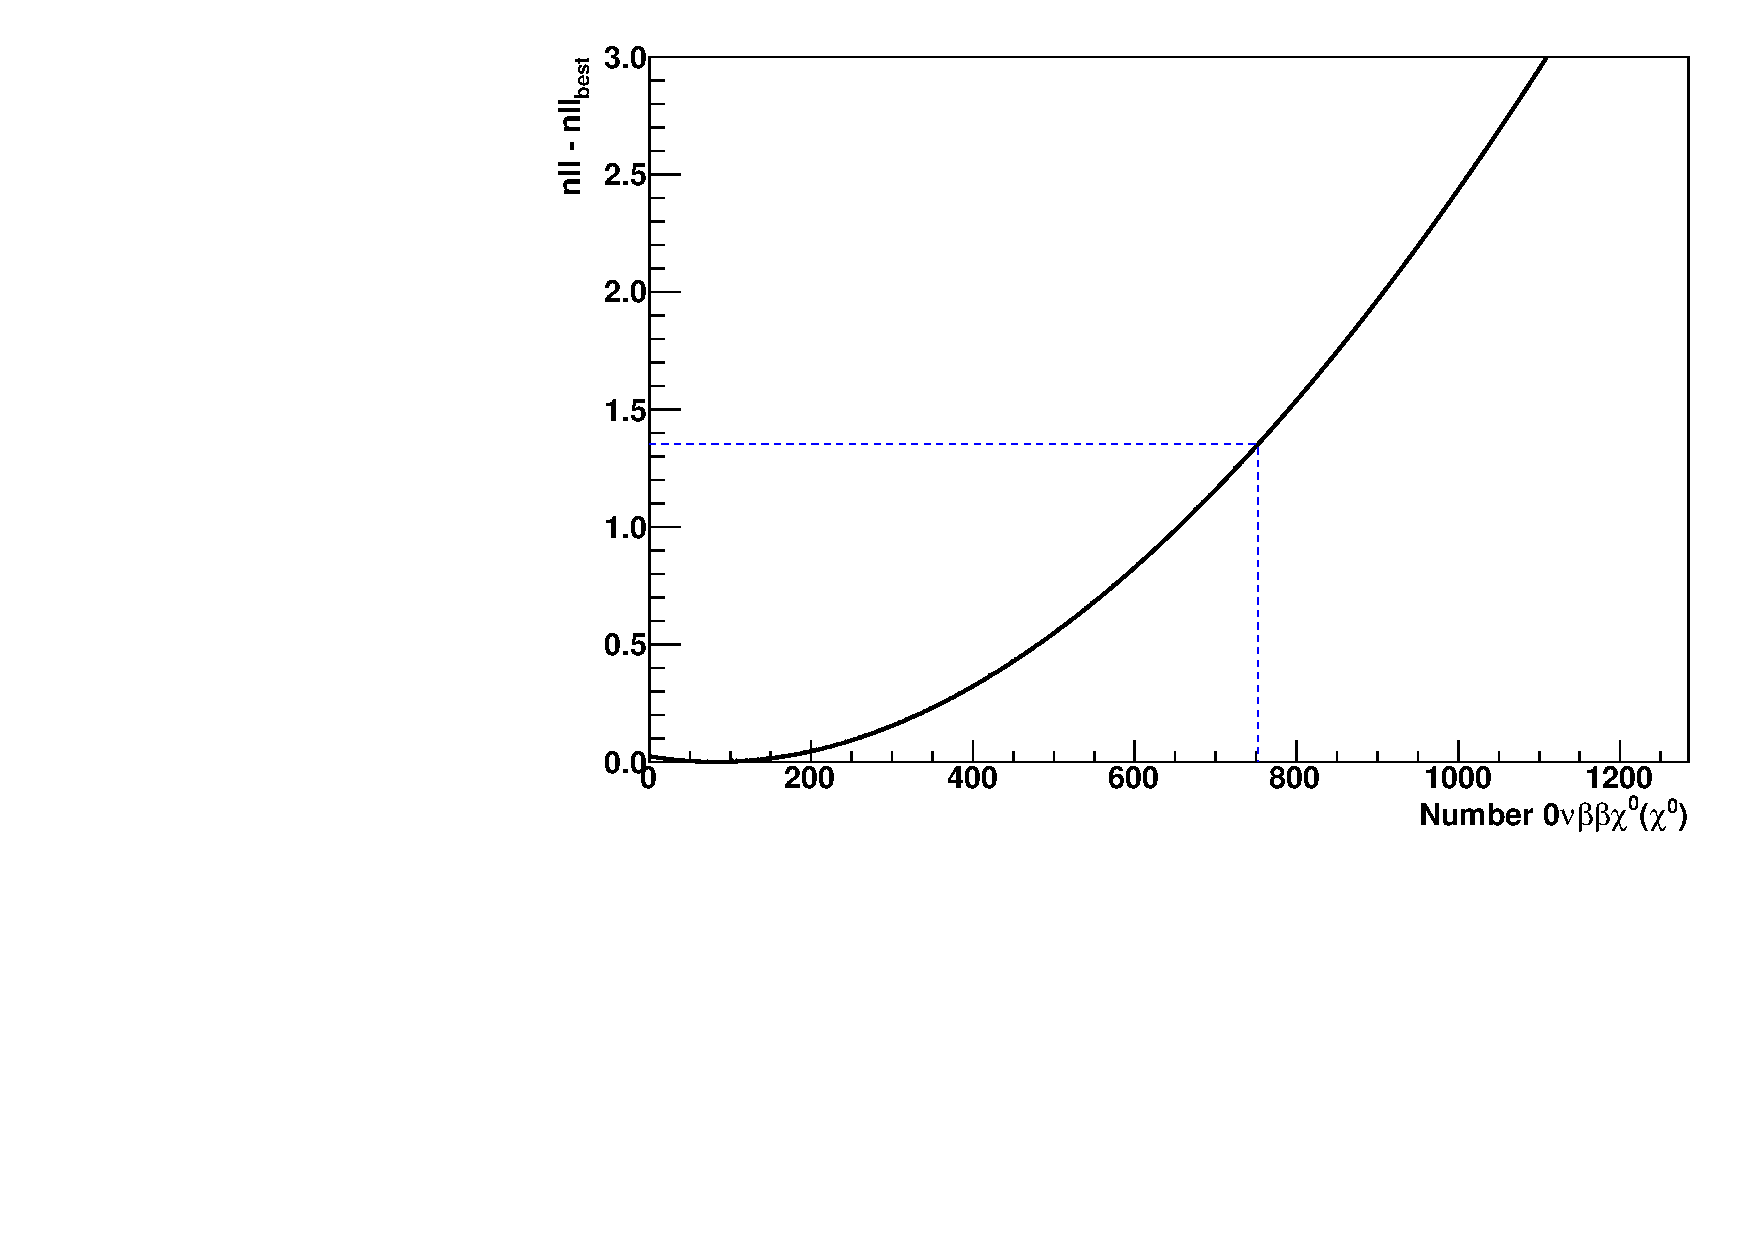
\includegraphics[width=\textwidth]{./plots/analysis_bb0nX3_profile.pdf}
	\end{subfigure}\hfill%
	\begin{subfigure}[c]{0.48\textwidth}
	\centering
	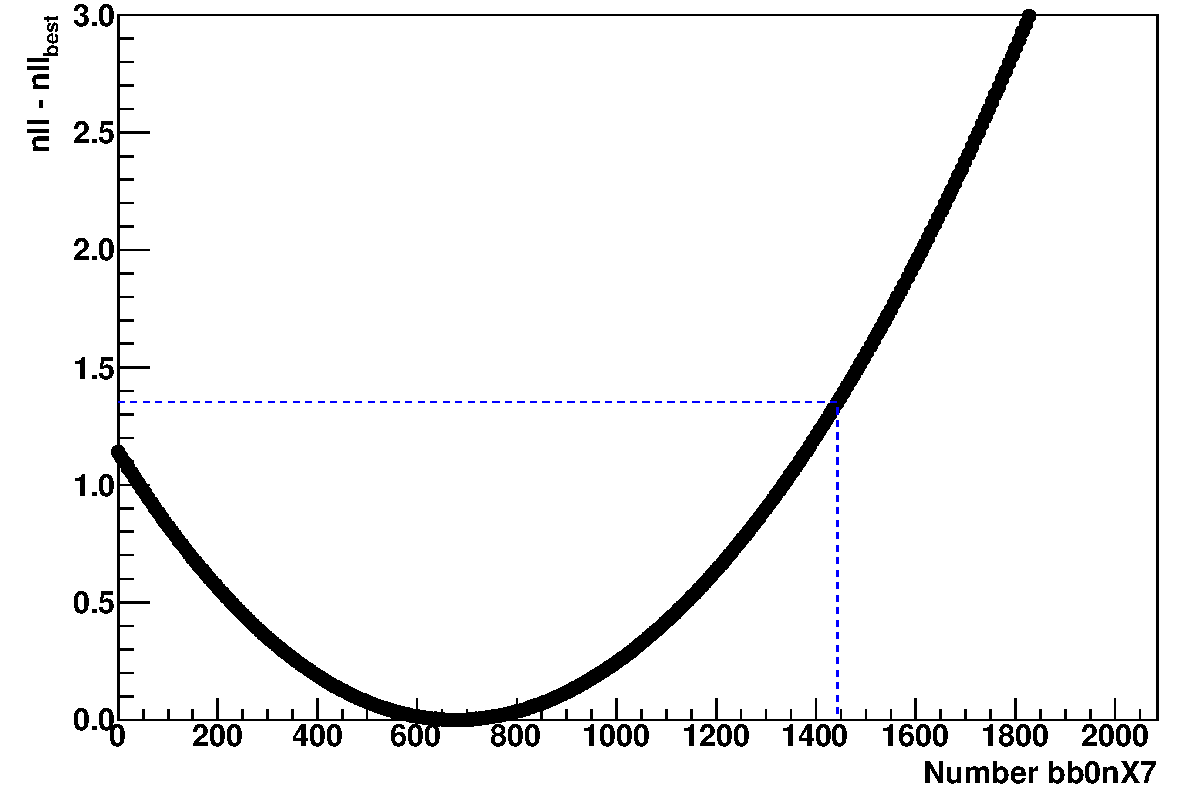
\includegraphics[width=\textwidth]{./plots/analysis_bb0nX7_profile.pdf}
	\end{subfigure}
\caption[Profile likelihoods for \(0\nu\beta\beta\chi^0(\chi^0)\)]{Profile likelihood scans for the Majoron-emitting modes. Though some modes fit to a non-zero value best fit, they are not significant at the 90\% confidence level. The change in negative log likelihood corresponding to the limit, and the limit, are shown in blue. Upper left is spectral index 1. Upper right is spectral index 2. Bottom left is spectral index 3. Bottom right is spectral index 7.}
\label{fig:analysis_bb0nX_profiles}
\end{figure}

\begin{figure}[htbp]
\centering
	\begin{subfigure}[c]{0.48\textwidth}
	\centering
	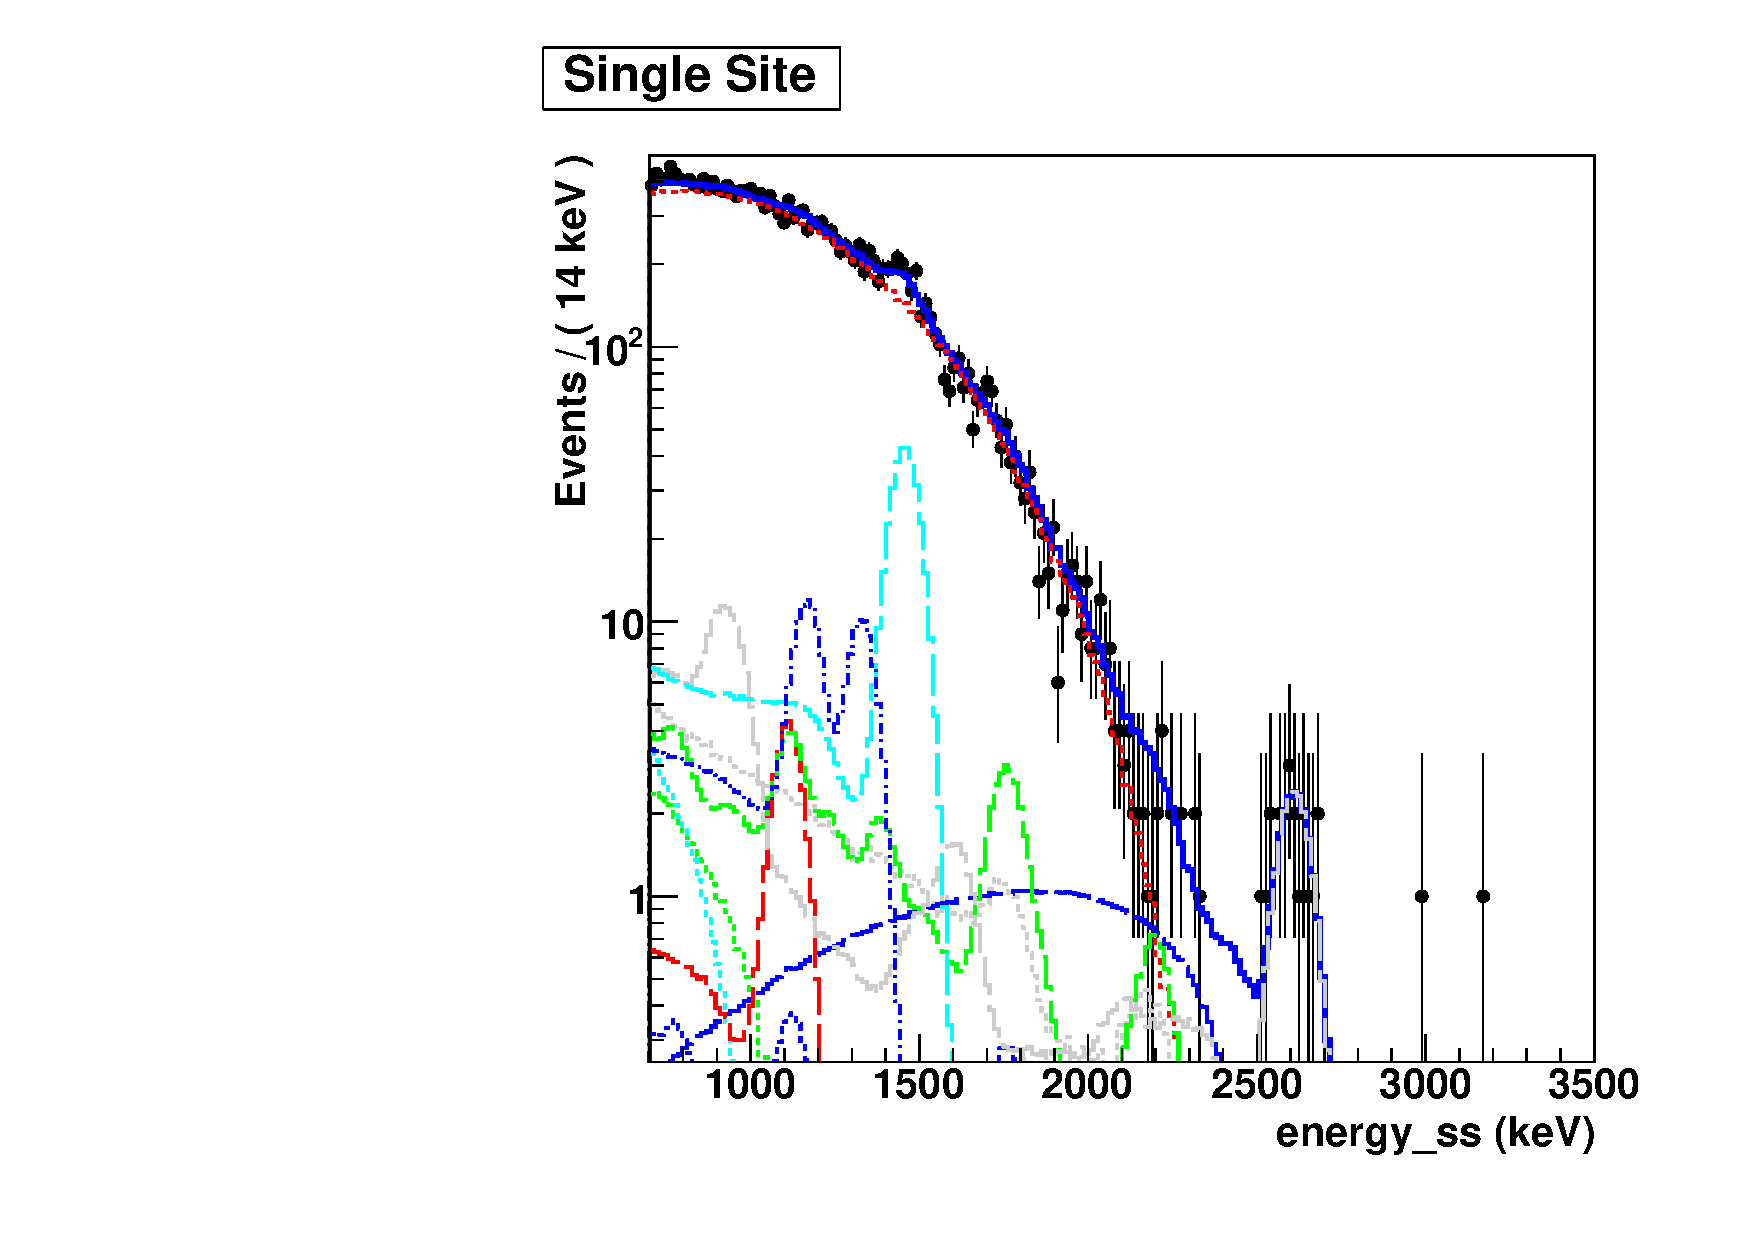
\includegraphics[width=\textwidth]{./plots/analysis_bb0nX1_90_fit_e_ss.pdf}
	\end{subfigure}\hfill%
	\begin{subfigure}[c]{0.48\textwidth}
	\centering
	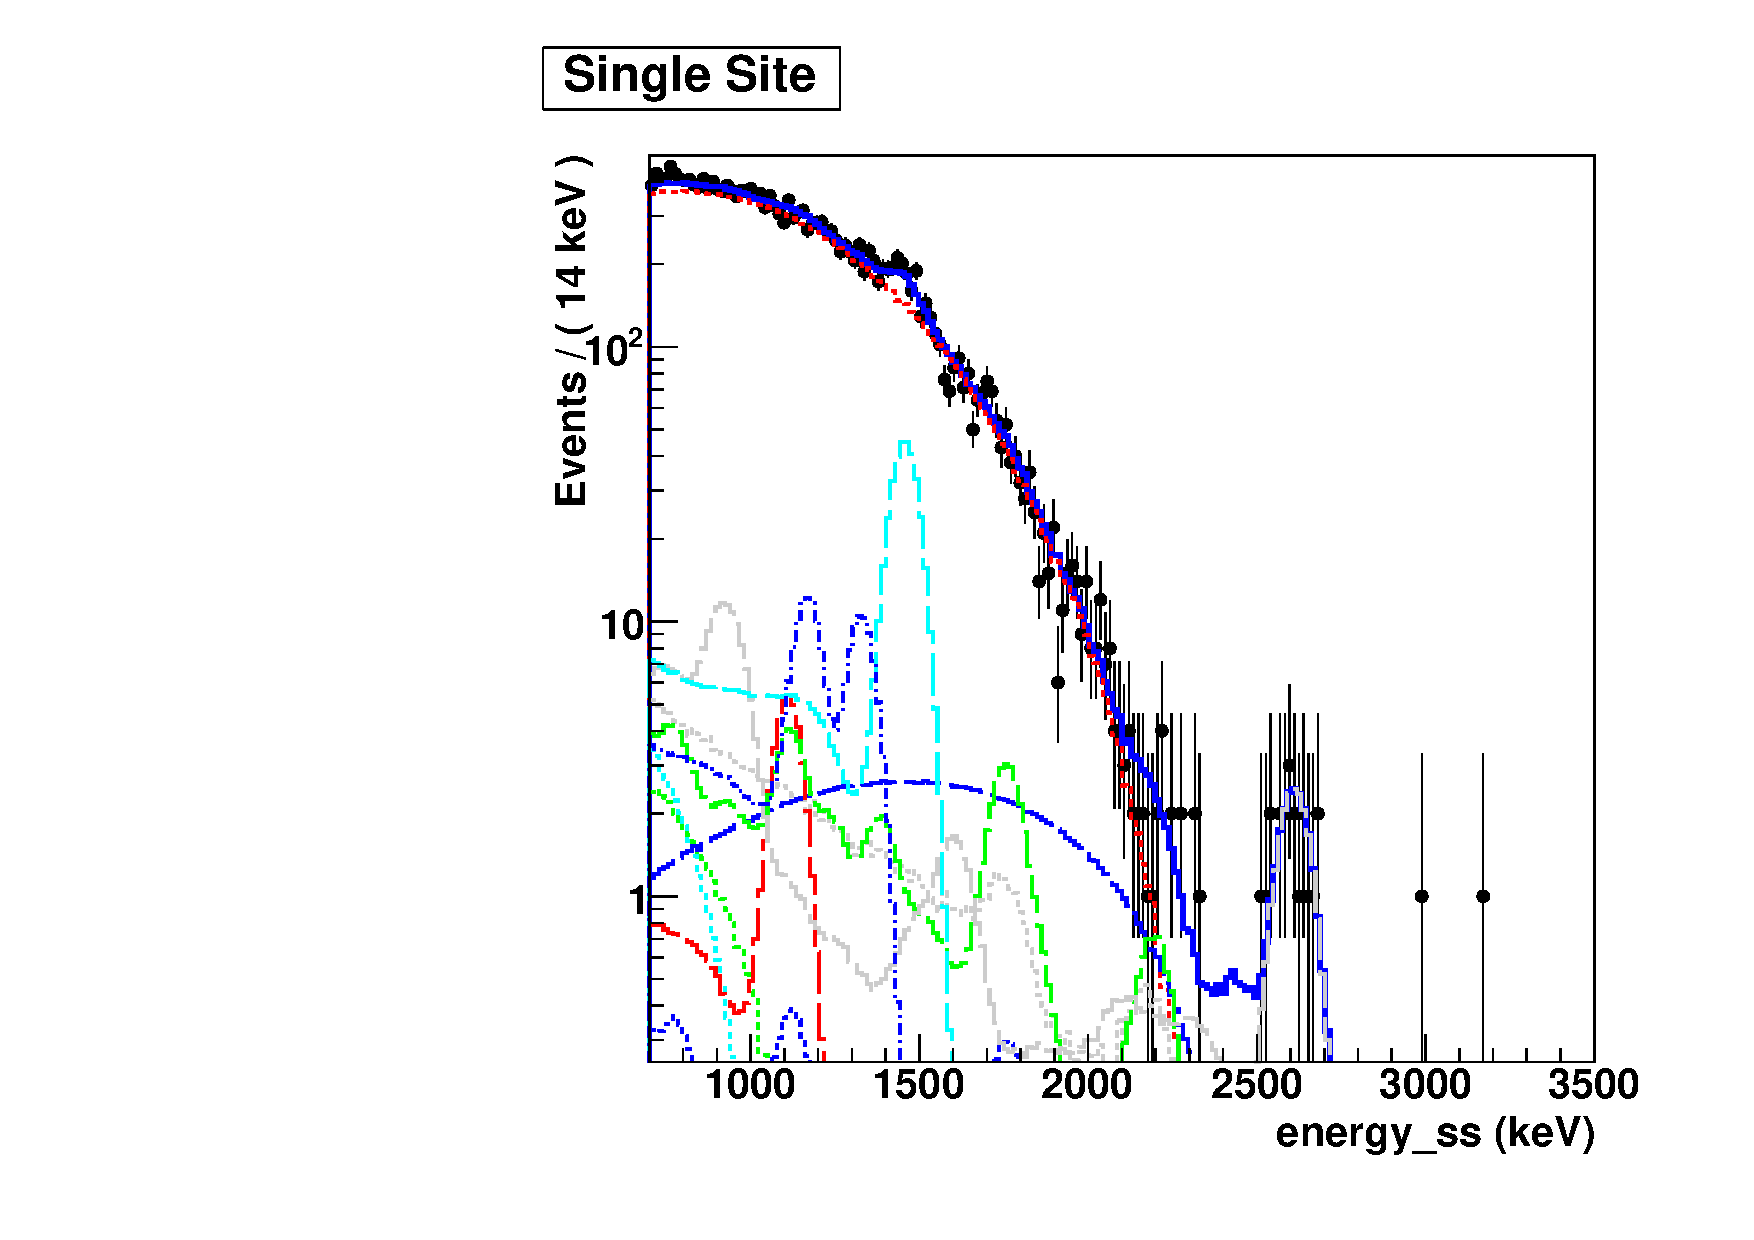
\includegraphics[width=\textwidth]{./plots/analysis_bb0nX2_90_fit_e_ss.pdf}
	\end{subfigure}
	\begin{subfigure}[c]{0.48\textwidth}
	\centering
	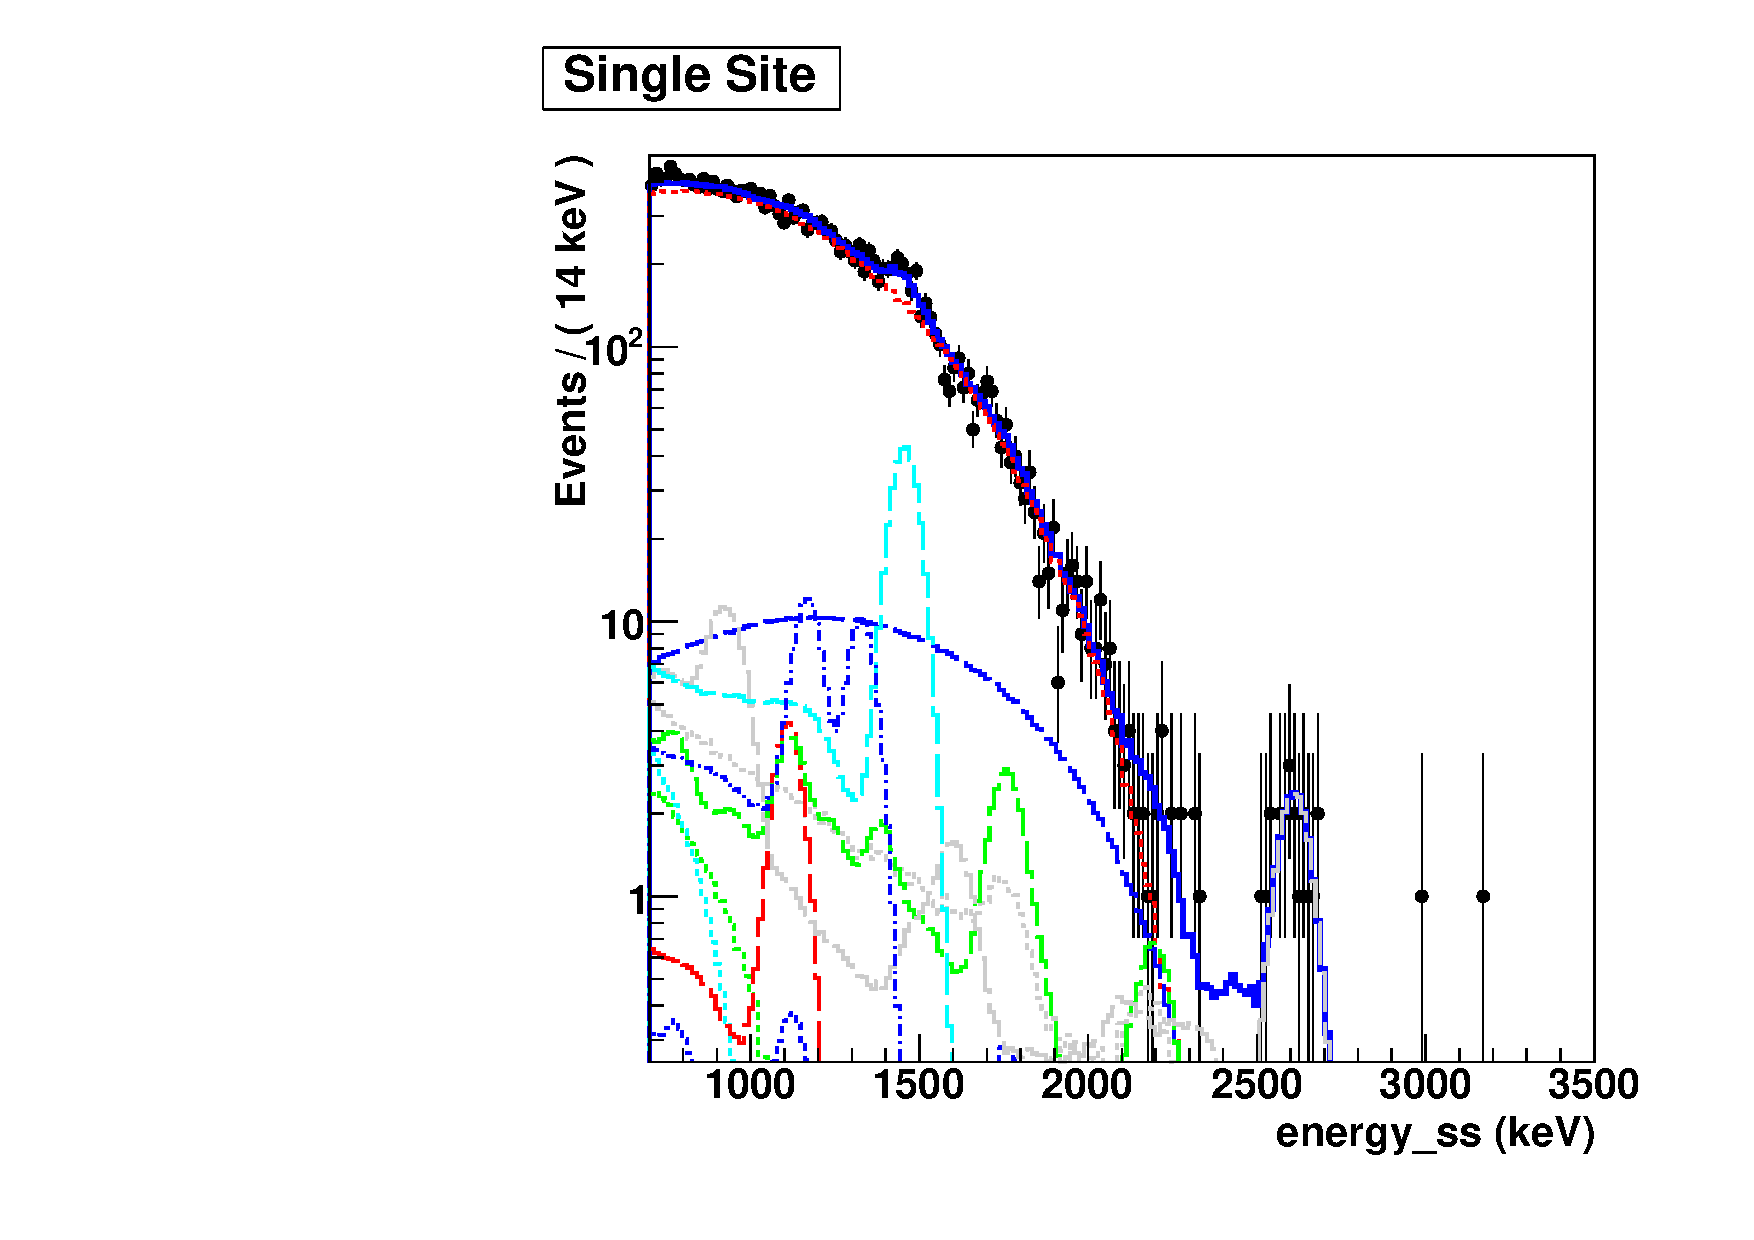
\includegraphics[width=\textwidth]{./plots/analysis_bb0nX3_90_fit_e_ss.pdf}
	\end{subfigure}\hfill%
	\begin{subfigure}[c]{0.48\textwidth}
	\centering
	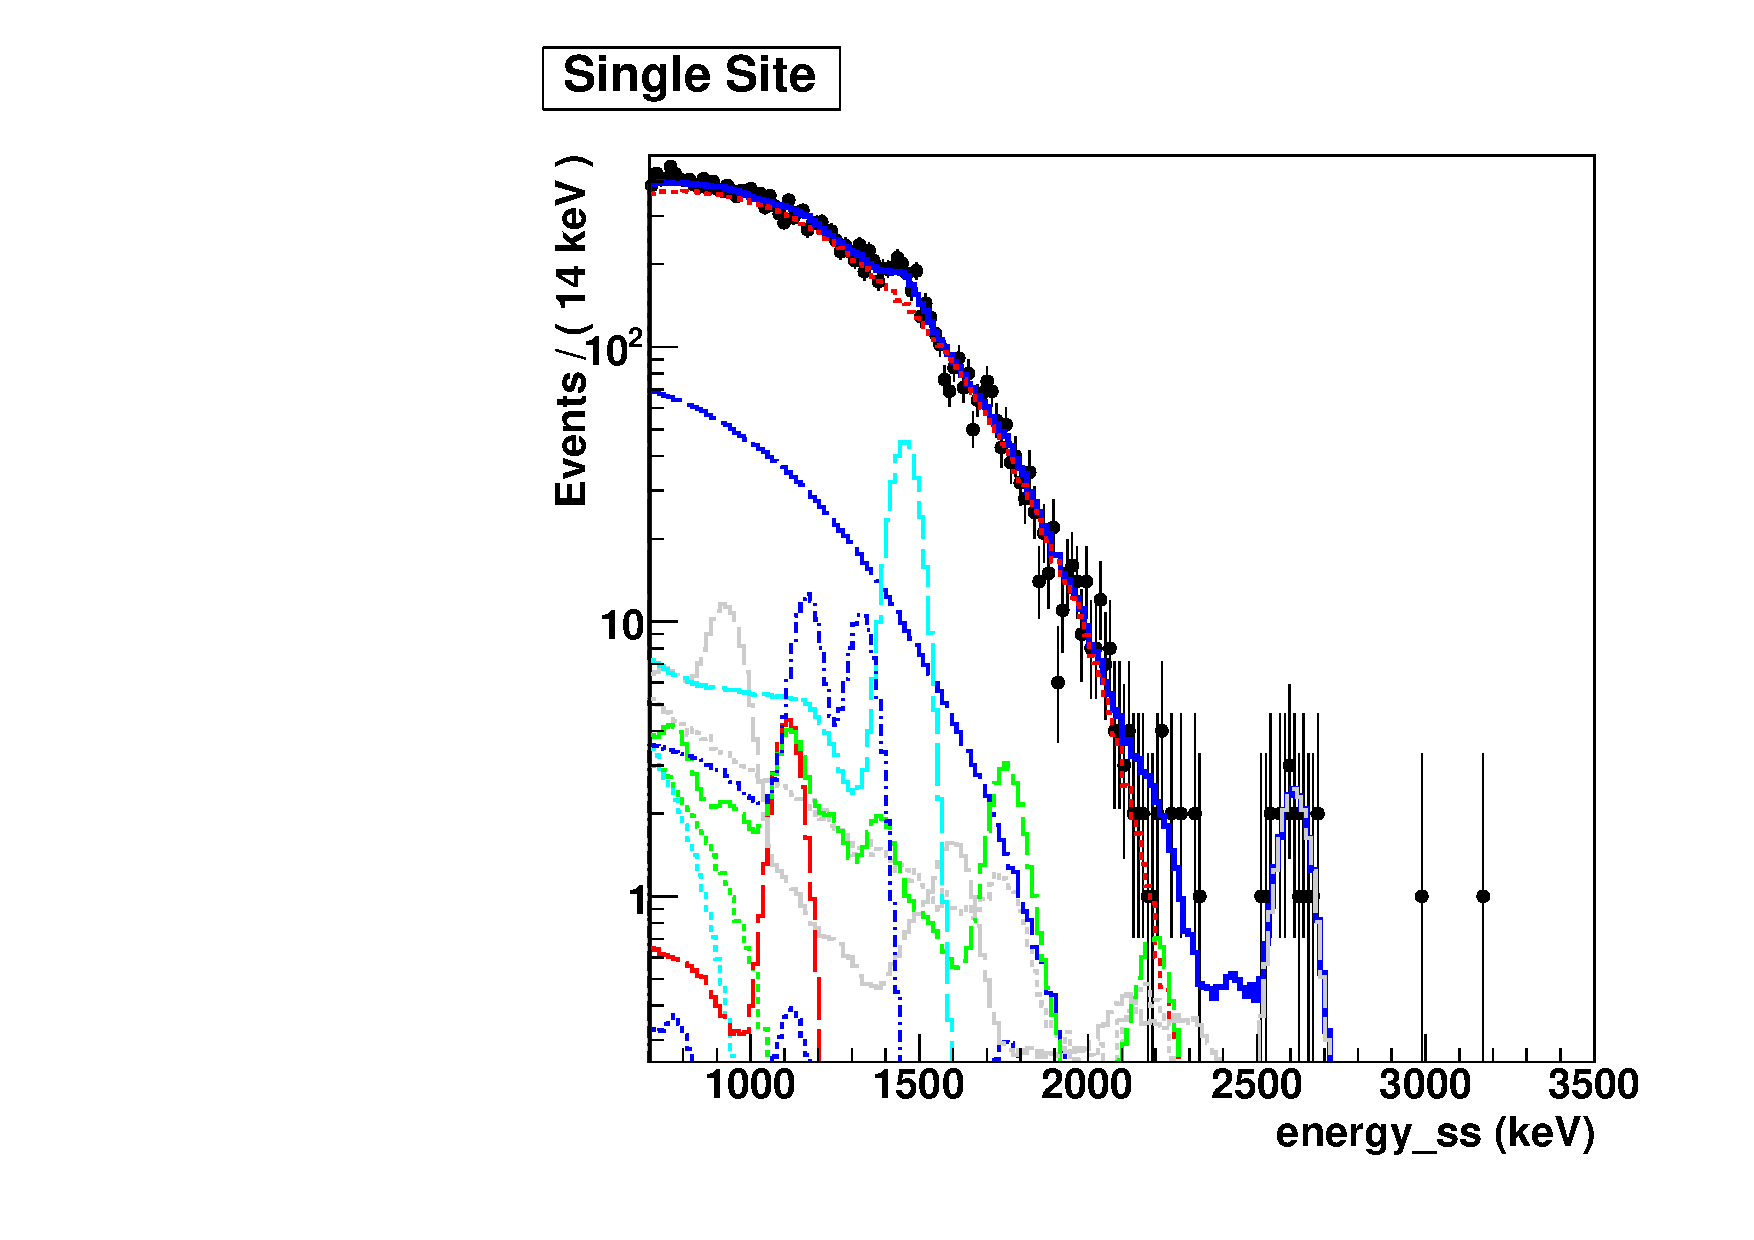
\includegraphics[width=\textwidth]{./plots/analysis_bb0nX7_90_fit_e_ss.pdf}
	\end{subfigure}
	\begin{subfigure}[c]{\textwidth}
	\centering
	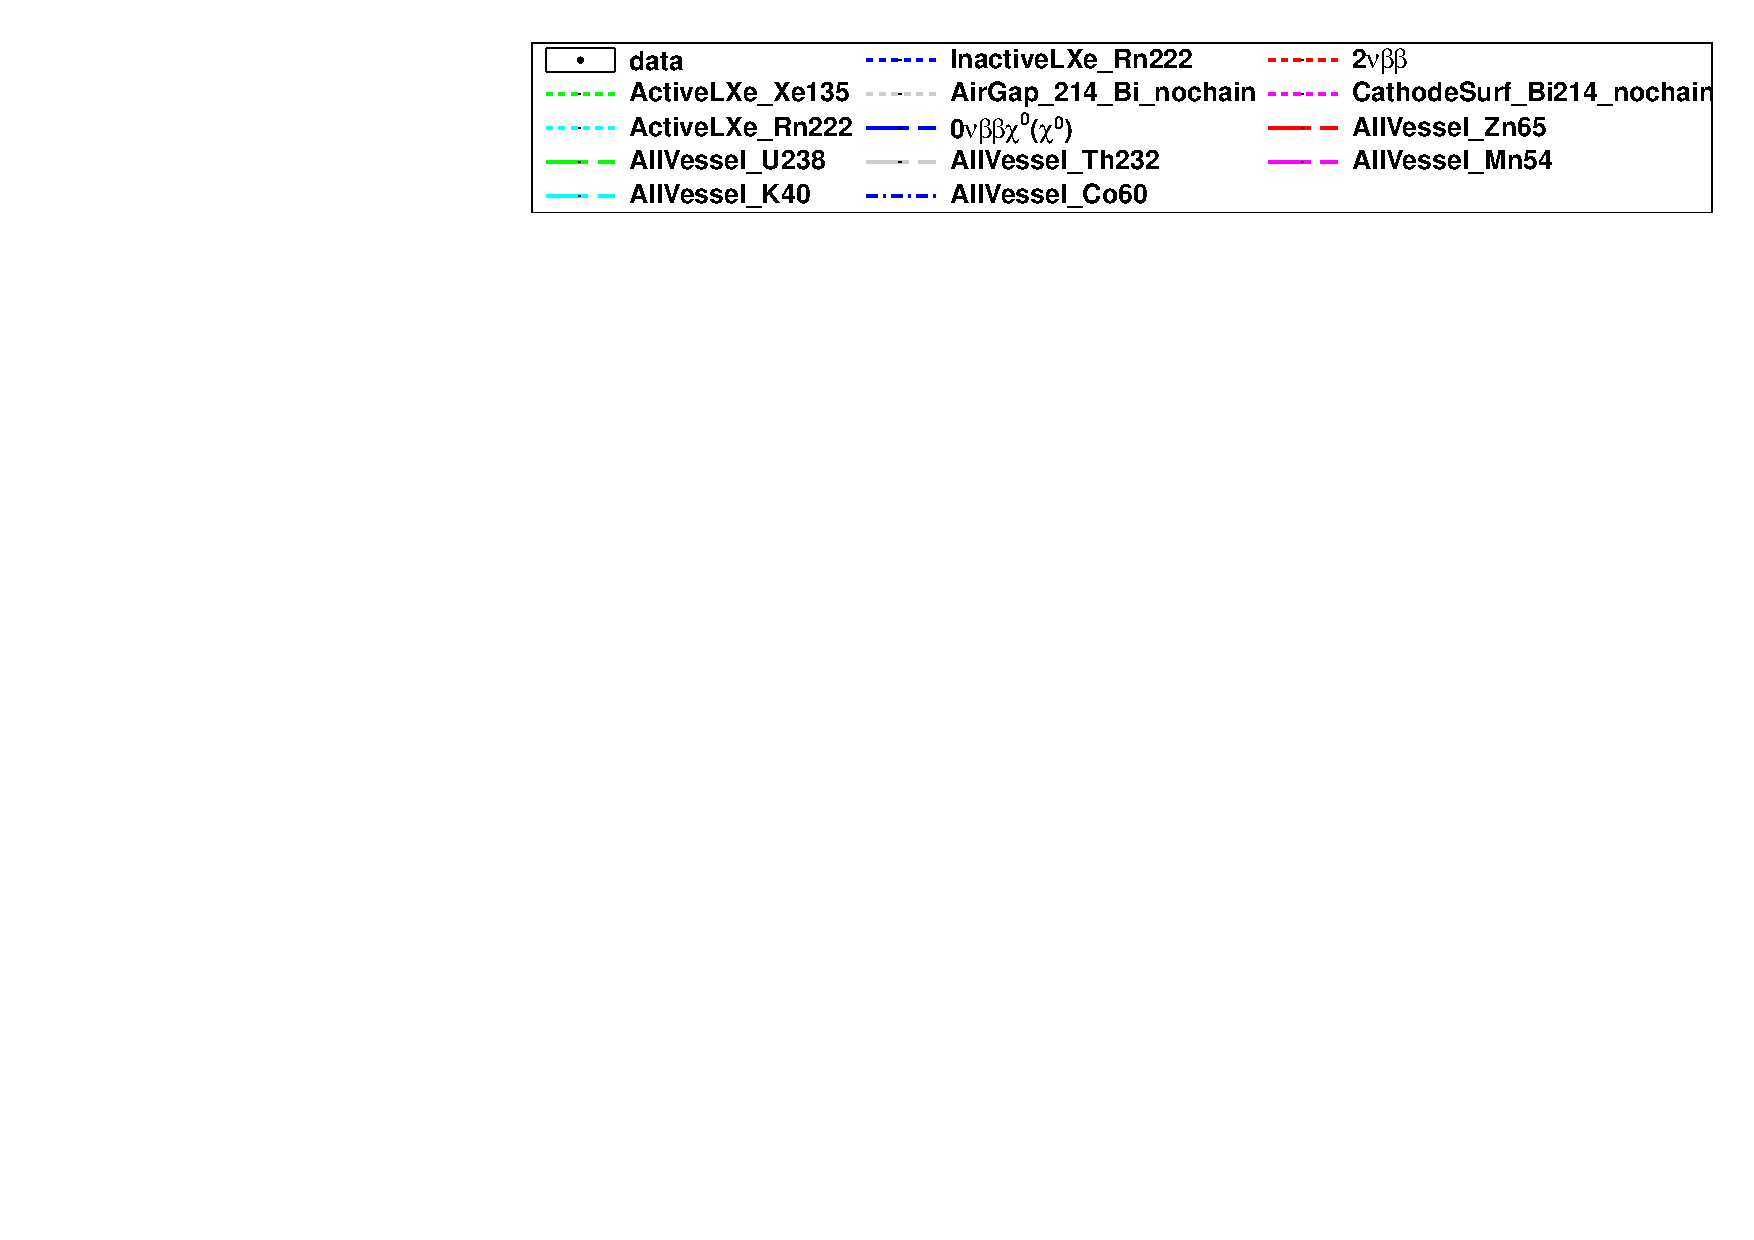
\includegraphics[width=\textwidth]{./plots/analysis_bb0nX_90_fit_legend.pdf}
	\end{subfigure}
\caption[Fits for \(0\nu\beta\beta\chi^0(\chi^0)\)]{The best fits of \twonu{}, \(0\nu\beta\beta\chi^0(\chi^0)\), and all background components to the data. Only projections of the single site energy spectra are shown. For each of the Majoron-emitting modes, the 90\% confidence level upper limit is shown. Upper left is spectral index 1. Upper right is spectral index 2. Bottom left is spectral index 3. Bottom right is spectral index 7.}
\label{fig:analysis_bb0nX_best_fit}
\end{figure}

\begin{table}[htbp]
\caption[Limits on Majoron-emitting mode half lives]{The half life limits obtained for the various Majoron emitting modes in \xenon{136} by KamLAND-Zen \cite{Gando:2012fk} and in this work. All limits are at the 90\% confidence level.}
\label{tab:analysis_majoron_limits}
\centering
\begin{tabular}{ l c c c}\toprule
Decay mode	&	n	&	\multicolumn{2}{c}{\(T_{1/2} (\si{\year})\)}					\\
			&		&	KamLAND-Zen		&	EXO-200 (this work)			\\\midrule
\zeronuX{}	&	1	&	\(>2.6\times10^{24}\)		&	\(>7.15\times10^{23}\)		\\
\zeronuX{}	&	2	&	\(>1.0\times10^{24}\)		&	\(>2.59\times10^{23}\)		\\
\zeronuXpX{}	&	3	&	\(>4.5\times10^{23}\)		&	\(>7.35\times10^{22}\)		\\
\zeronuXX{}	&	7	&	\(>1.1\times10^{22}\)		&	\(>1.33\times10^{22}\)		\\\bottomrule
\end{tabular}
\end{table}

\subsection{Effect of Systematic Uncertainties}
\label{sec:analysis_majoron_error_budget}
\Cref{tab:analysis_majoron_error_budget} tabulates the effect of the various uncertainties on the limits obtained for the Majoron-emitting modes. All of the limits are only slightly degraded below their statistical limits. For all modes, uncertainty in the backgrounds has a modest effect on the limit. Being able to better constrain the backgrounds, both through external constraints and more detector data, could improve the limits. For all modes, the statistical limits are weakened more by the uncertainty in the single site fraction. Since these events are similar to \twonu{} events, this suggests the limits could be improved modestly by using the \twonu{} single site fraction as a constraint on the single site fraction for these modes. The normalization uncertainty does not weaken the limit significantly, and so enlarging the fiducial volume to increase the number of xenon atoms would likely improve the limit, despite worsening the normalization uncertainty.

\begin{table}[htbp]
\centering
\caption[Effects of uncertainties to the limits on Majoron-emitting modes]{A breakdown of how various uncertainties effect the limit obtained on the Majoron-emitting modes. These are obtained by fixing parameters to their best-fit values and then letting only the specified parameters float when doing the profile scan. \twonu{} is considered a background for these results.}
\label{tab:analysis_majoron_error_budget}
\begin{tabular}{c c c c c }\toprule
Uncertainty		&	\multicolumn{4}{c}{90\% CL limit on \(T_{1/2}\)}			\\
				&	\(n = 1\) (\SI{e23}{\year})		&	\(n = 2\) (\SI{e23}{\year})		&	\(n = 3\) (\SI{e22}{\year})		&	\(n=7\) (\SI{e22}{\year})	\\\midrule
Statistical only	&	7.42						&	2.71						&	7.99						&	1.38					\\
SS fraction	&	7.22						&	2.62						&	7.50						&	1.37					\\
Backgrounds	&	7.39						&	2.69						&	7.92						&	1.36					\\
Normalization	&	7.42						&	2.71						&	7.99						&	1.38					\\\midrule
\textbf{Reported}&	\textbf{7.15}				&	\textbf{2.59}				&	\textbf{7.35}				&	\textbf{1.33}			\\\bottomrule
\end{tabular}
\end{table}

\subsection{Coverage Tests and Sensitivity}
As discussed in \cref{sec:analysis_ml_theory}, when using the bounded likelihood method of Rolke et al., it is important to verify that the intervals constructed have coverage. To study this, the best fit spectrum with no \zeronuXpX{} decays included is used to generate toy Monte Carlo data sets. Sampling from the \zeronuXpX{} PDF, a known number of events are injected into the toy data set, and the profile likelihood method is used to construct confidence intervals. Doing this many times provides an estimate of how likely the intervals are to cover the true value. As \cref{fig:analysis_bb0nX_coverage} shows, the method provides adequate coverage.

\begin{figure}[tbp]
\centering
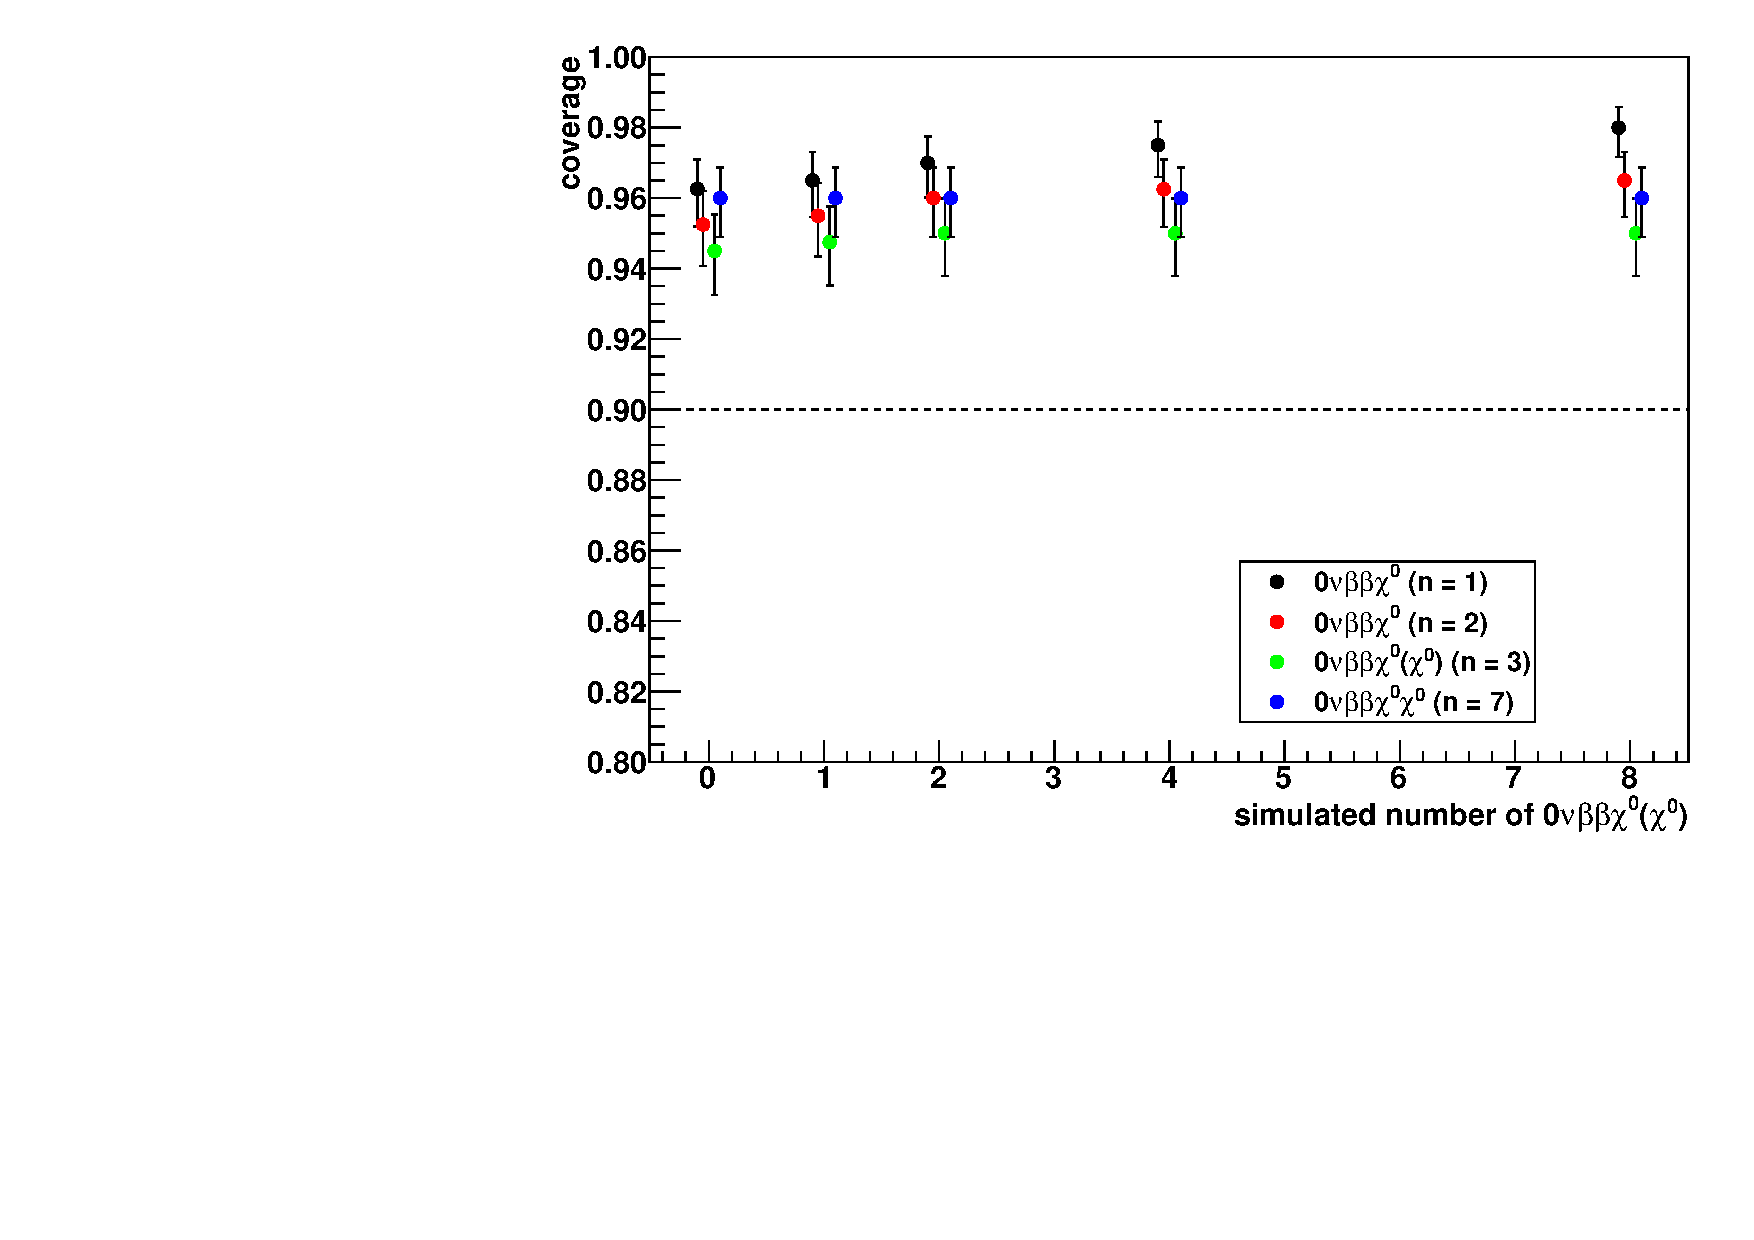
\includegraphics[width=0.7\textwidth]{./plots/analysis_bb0nX_coverage.pdf}
\caption[Coverage tests for \zeronuXpX{}]{The results of coverage tests for the confidence intervals produced by the fits for Majoron-emitting modes when setting a limit. For a nominal 90\% confidence level, good coverage is shown for all modes, though some exhibit overcoverage. Each point represents the coverage fraction for 400 tests with the indicated number (0, 1, 2, 4, or 8) of \zeronuXpX{} events injected. In all cases, an integral number of events were injected; the points are spaced out for ease of visualization.}
\label{fig:analysis_bb0nX_coverage}
\end{figure}

\begin{figure}[tbp]
\centering
	\begin{subfigure}[c]{0.48\textwidth}
	\centering
	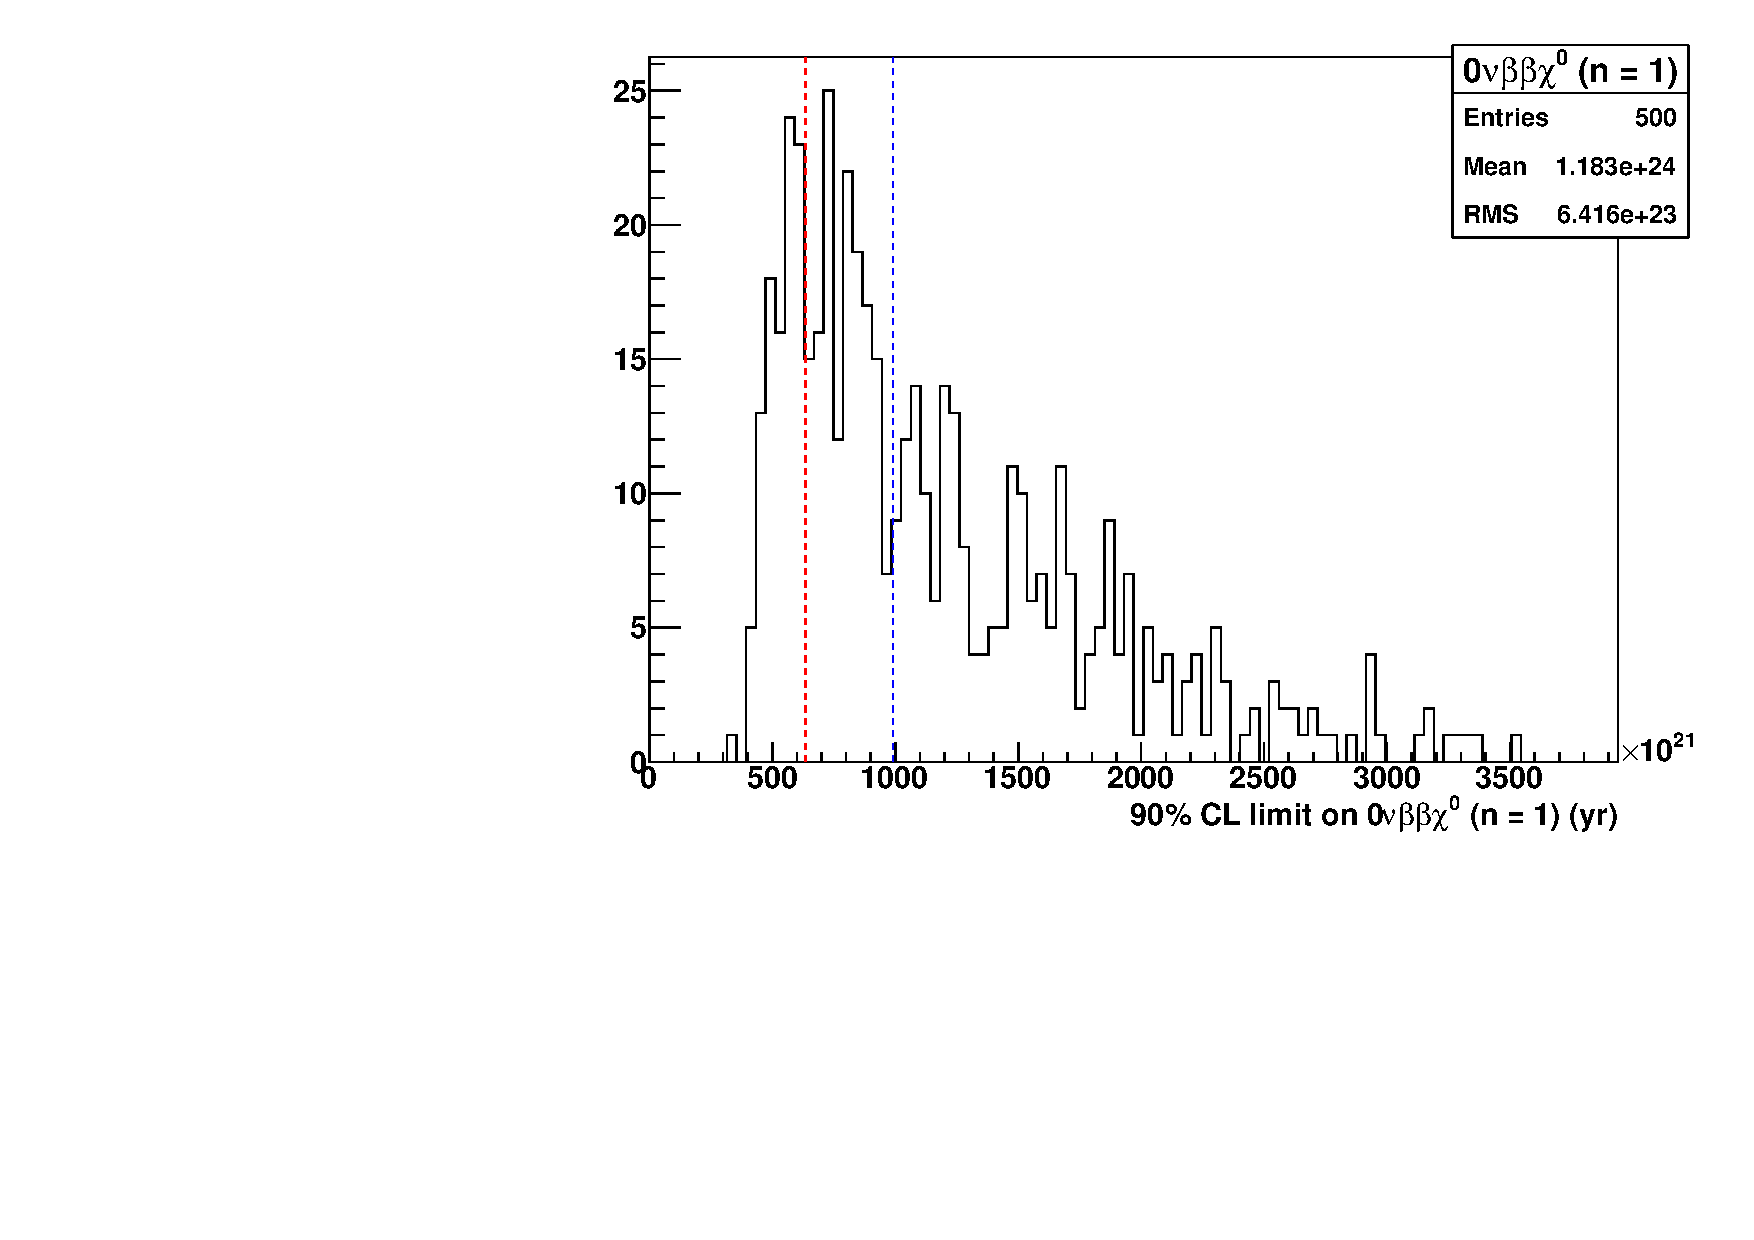
\includegraphics[width=\textwidth]{./plots/analysis_bb0nX1_sensitivity.pdf}
	\end{subfigure}\hfill%
	\begin{subfigure}[c]{0.48\textwidth}
	\centering
	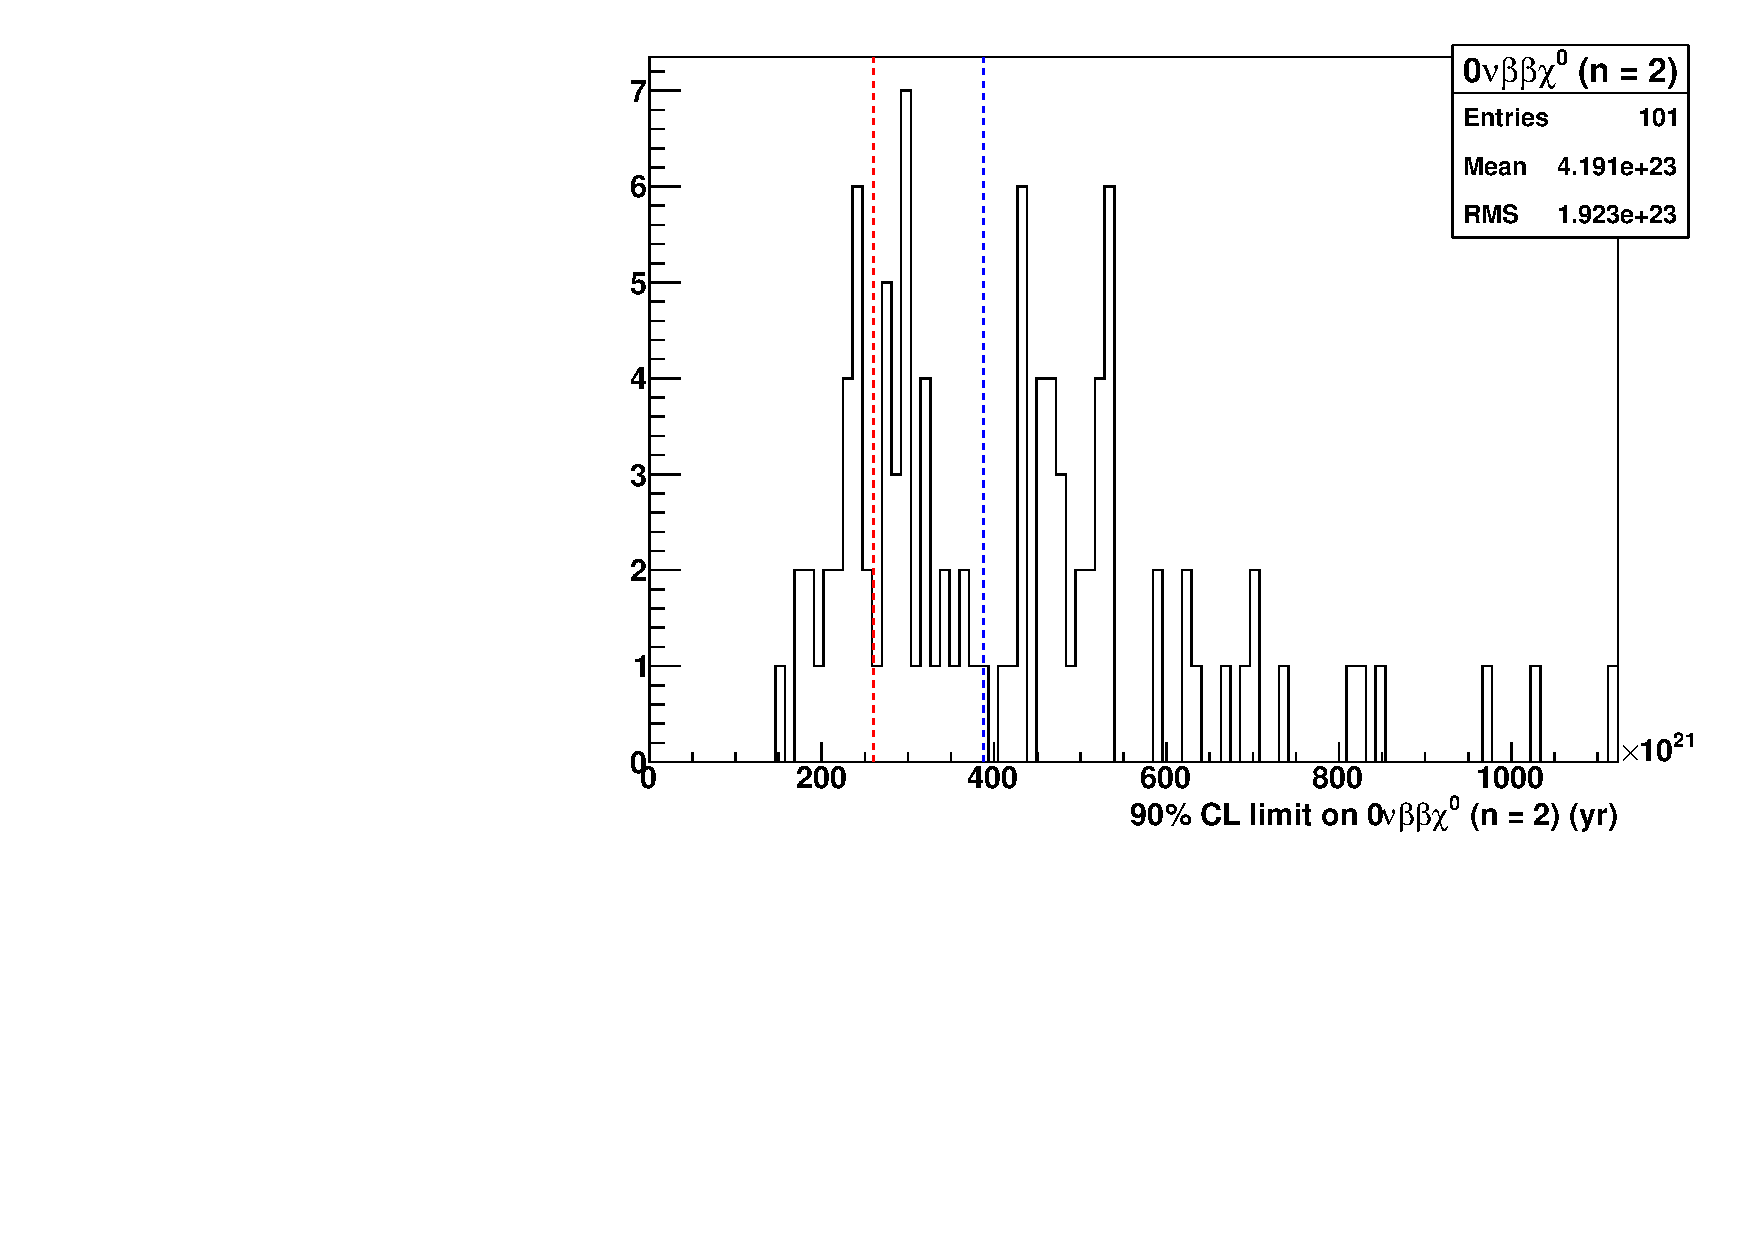
\includegraphics[width=\textwidth]{./plots/analysis_bb0nX2_sensitivity.pdf}
	\end{subfigure}
	\begin{subfigure}[c]{0.48\textwidth}
	\centering
	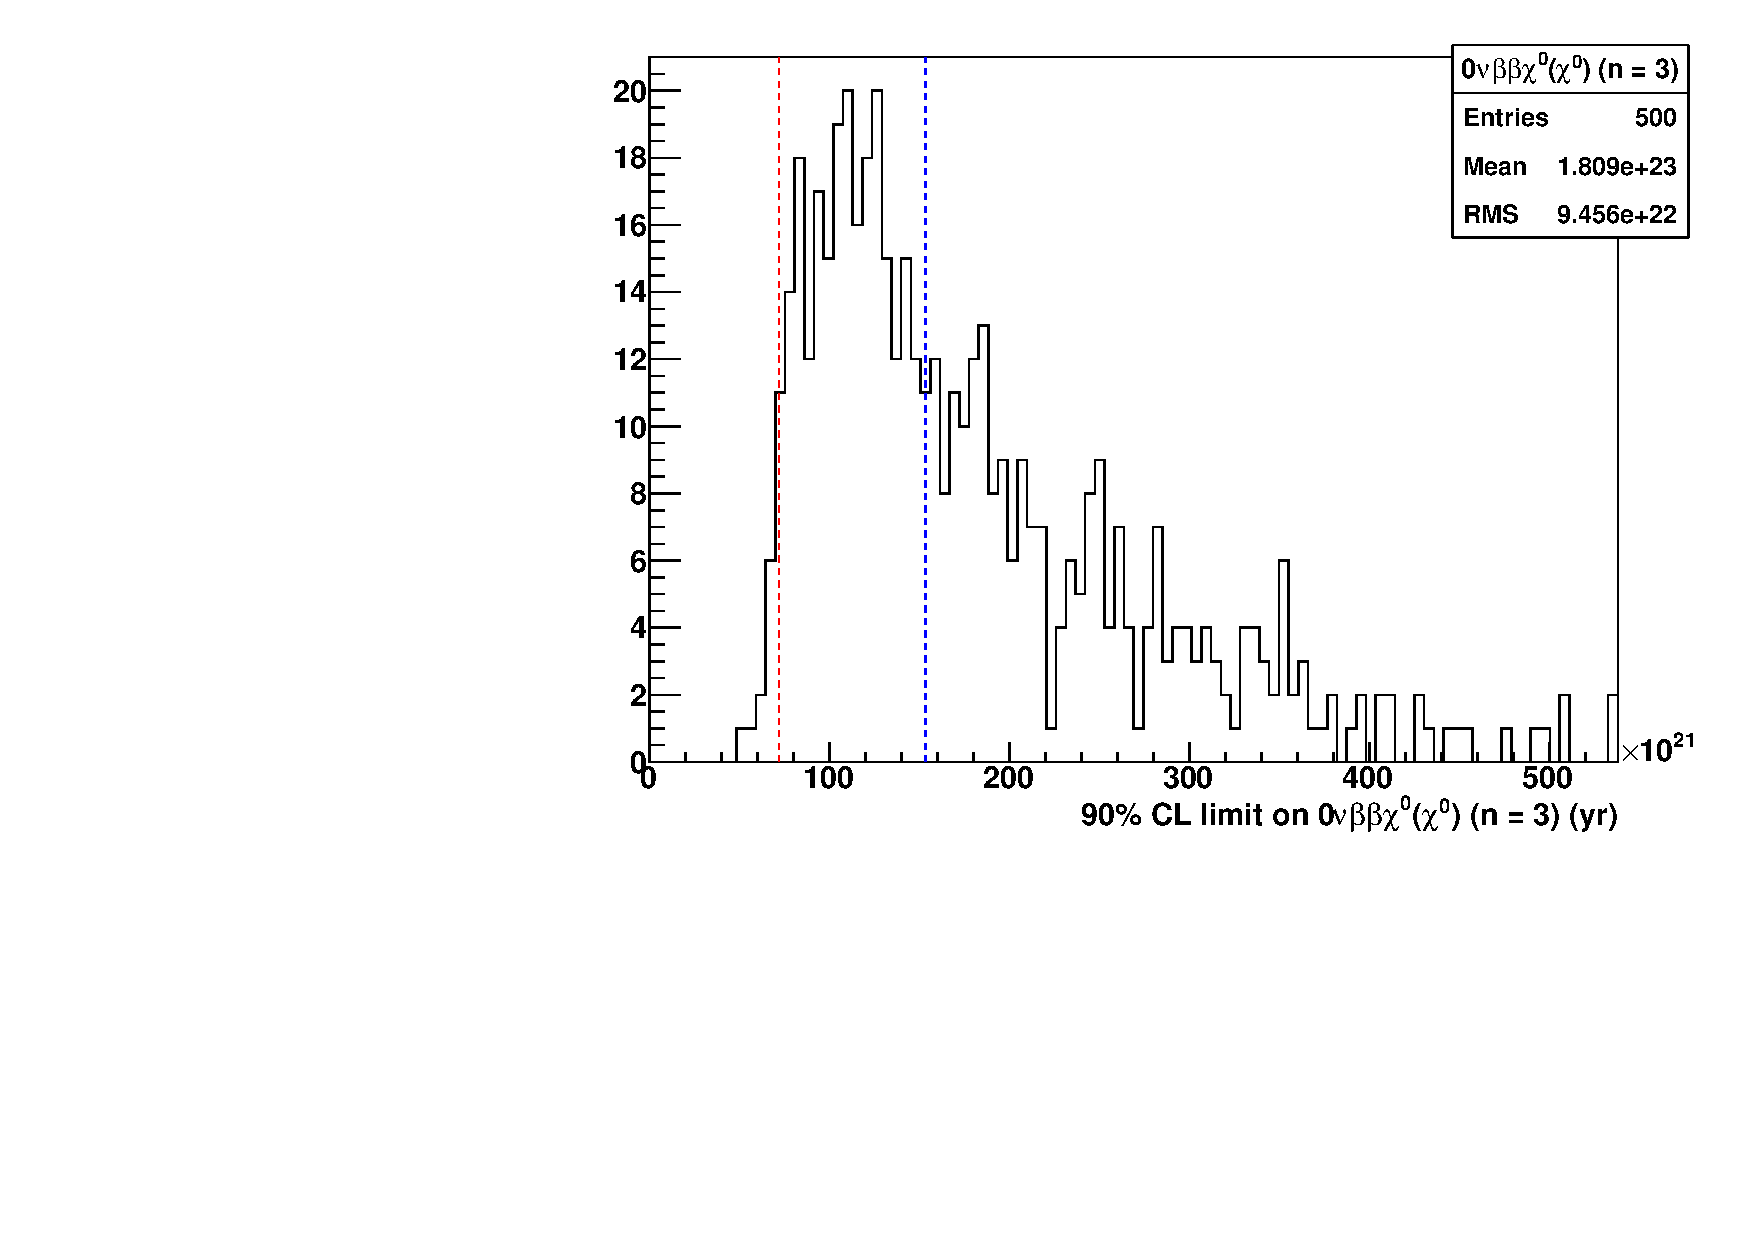
\includegraphics[width=\textwidth]{./plots/analysis_bb0nX3_sensitivity.pdf}
	\end{subfigure}\hfill%
	\begin{subfigure}[c]{0.48\textwidth}
	\centering
	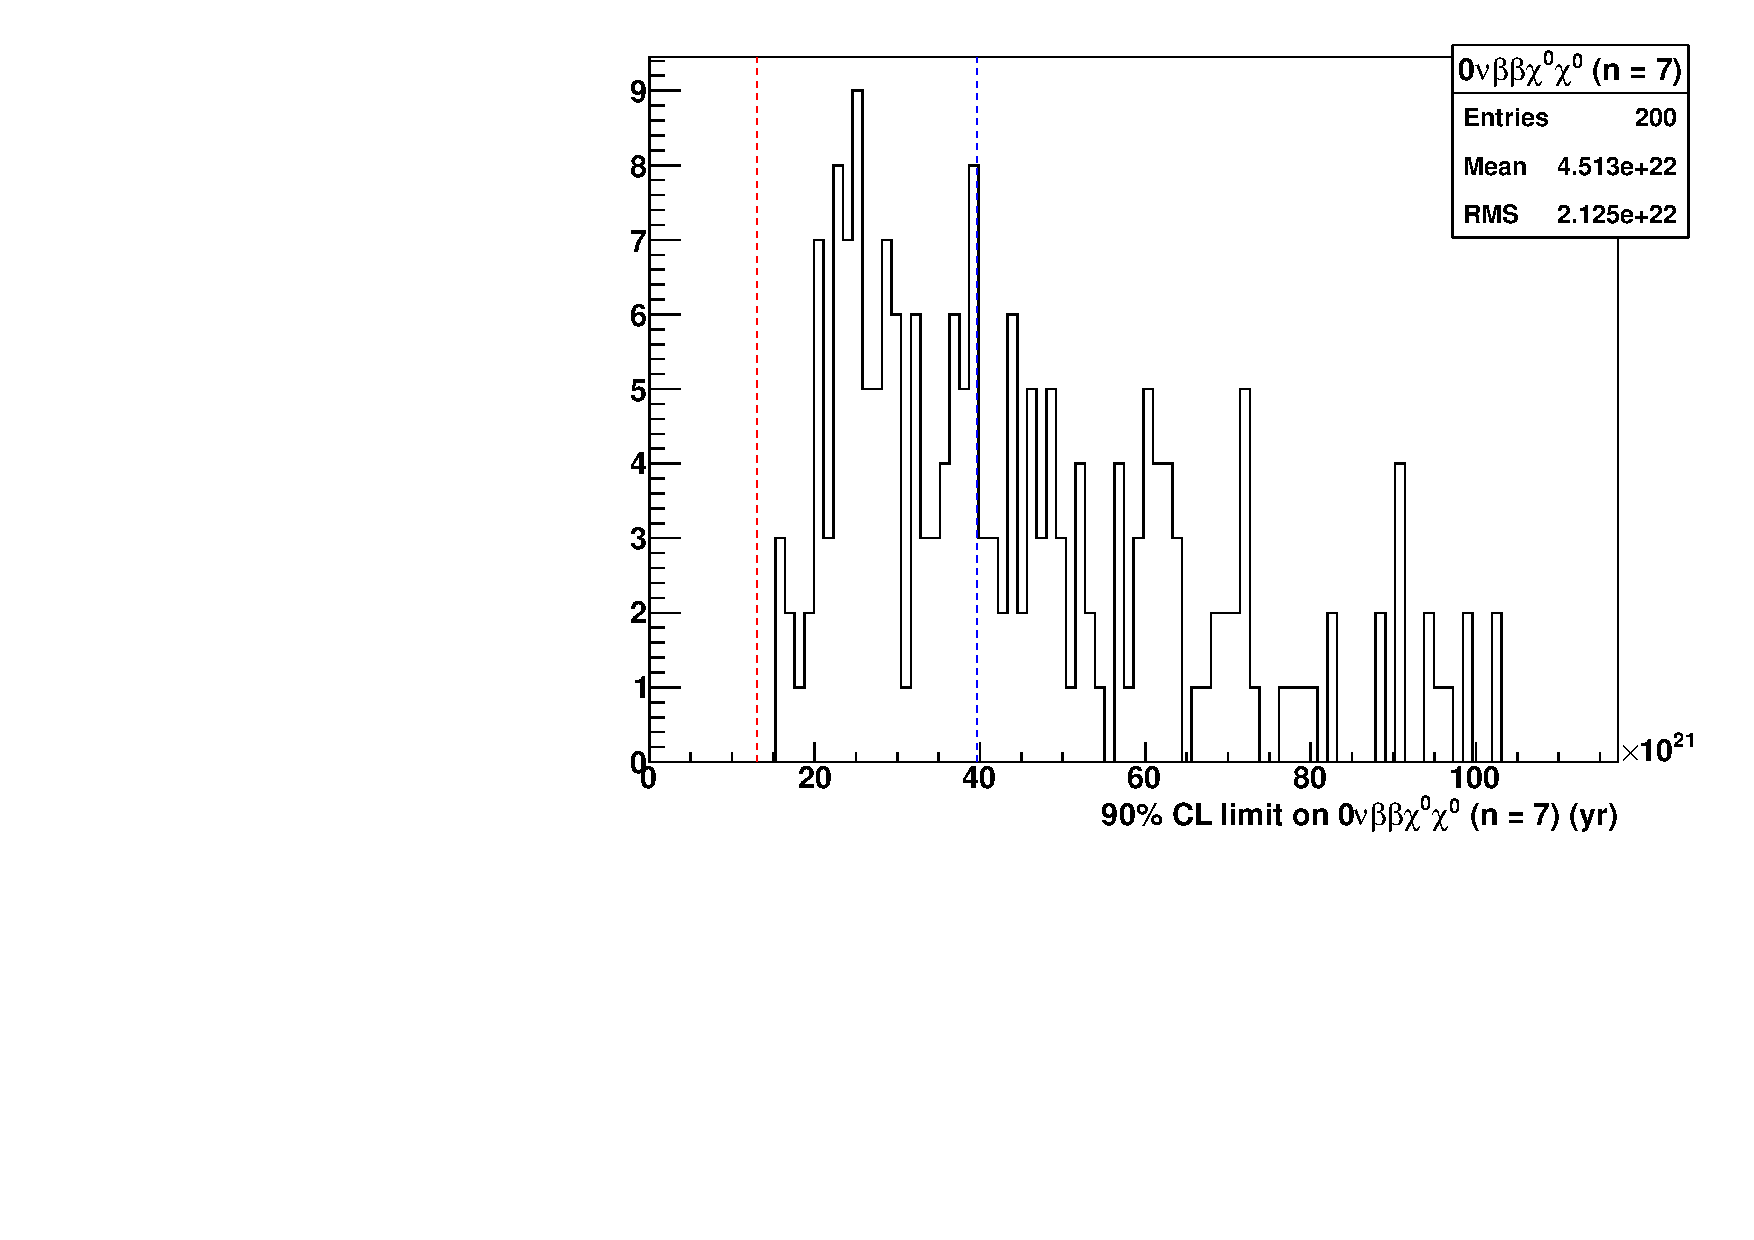
\includegraphics[width=\textwidth]{./plots/analysis_bb0nX7_sensitivity.pdf}
	\end{subfigure}
\caption[Sensitivity studies for \(0\nu\beta\beta\chi^0(\chi^0)\)]{The limits obtained for toy simulations containing zero Majoron-emitting events, made from the best-fit to the data. The median limit is shown in blue, while the obtained limit is shown in red.}
\label{fig:analysis_bb0nX_sensitivity}
\end{figure}

Using the best fit spectrum with no \zeronuXpX{} to again create toy simulations, it is possible to study the sensitivity to Majoron-emitting modes. Each simulation is used to construct a 90\% confidence interval. \Cref{fig:analysis_bb0nX_sensitivity} shows histograms of the limits obtained from many simulations. For all modes, the expected sensitivity is higher than the observed limit. For the modes with spectral indices 1 and 2, higher limits are expected 73\% and 78\% of the time, respectively. For the mode with spectral index 3, 95\% of simulations had a better limit. For the mode with spectral index 7, only two simulations in 500 had a comparable limit. Higher limits would be expected nearly all of the time. This suggests that the model used to simulate the data is inadequate. As discussed in \cref{sec:analysis_shape_agreement} the simulations show a slightly different single-site fraction than seen in data. Since the \zeronuXX{} spectrum is primarily single site and peaks at lower energies than \twonu{}, the upper limit on the number of decays is larger in data than in the toy simulations.

\subsection{Comparison to Previous Results}
As \cref{tab:analysis_majoron_limits} shows, the limits on the Majoron-emitting modes with spectral indices 1, 2, and 3 are weaker than those reported by KamLAND-Zen. The weaker limits are primarily due to statistics, as discussed in \cref{sec:analysis_majoron_error_budget}. This is not surprising, as the KamLAND-Zen results come from \SI{38.4}{\kg\year} exposure of \xenon{136}, whereas this analysis only contains \SI{21.0}{\kg\year}. For the spectral index 7 mode, EXO-200 can report a modestly improved limit. Looking at \cref{fig:analysis_kamlandzen_spectrum}, backgrounds in KamLAND-Zen begin to dominate over the \twonu{} mode below \SI{1}{\MeV}. EXO-200, on the other hand, has much smaller backgrounds at this low energy, which allow a stronger limit, even with reduced exposure.

\begin{figure}[htbp]
\centering
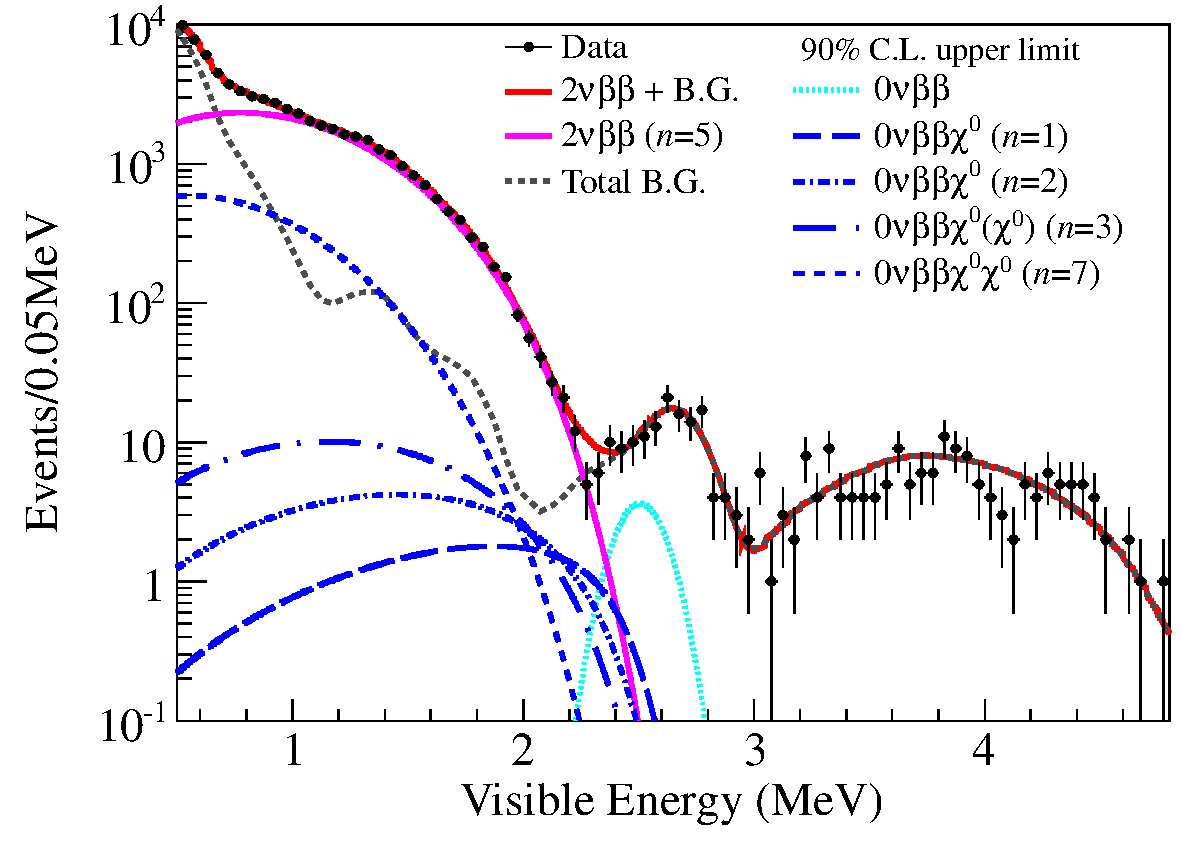
\includegraphics[width=0.7\textwidth]{./plots/analysis_kamlandzen_spectrum.pdf}
\caption[KamLAND-Zen spectrum for Majoron-emitting modes]{The energy spectrum reported by KamLAND-Zen. Backgrounds begin to become comparable to the \twonu{} signal below \SI{1}{\MeV}, reducing sensitivity to the Majoron-emitting mode with spectral index 7. Figure from \cite{Gando:2012fk}.}
\label{fig:analysis_kamlandzen_spectrum}
\end{figure}


\end{document}
